
\documentclass{beamer}

\usepackage[english]{babel}
\usepackage[utf8x]{inputenc}

\mode<presentation>
{
  \usetheme{Rochester}
  \usecolortheme{default}
}

\AtBeginSection[]
{
  \begin{frame}{Outline}
    \tableofcontents[currentsection]
  \end{frame}
}

\usepackage{graphicx}

\setbeamersize{text margin left=5mm,text margin right=5mm} 

\title{Informativity on $A_V$ (mutual information)}
\author{Lucas Einig}
\institute{IRAM - GIPSA-lab}
\date{\today}

\begin{document}

\begin{frame}
  \titlepage
\end{frame}

\begin{frame}{Outline}
  \tableofcontents
\end{frame}


\section{Combinations including $\mathrm{^{13}CO\,(1-0)}$ (11 available)}

\begin{frame}{Informativity on $A_V$ of $\left(\mathrm{^{12}CN\,(1-0)},\mathrm{^{13}CO\,(1-0)}\right)$}
    \begin{figure}
        \centering
        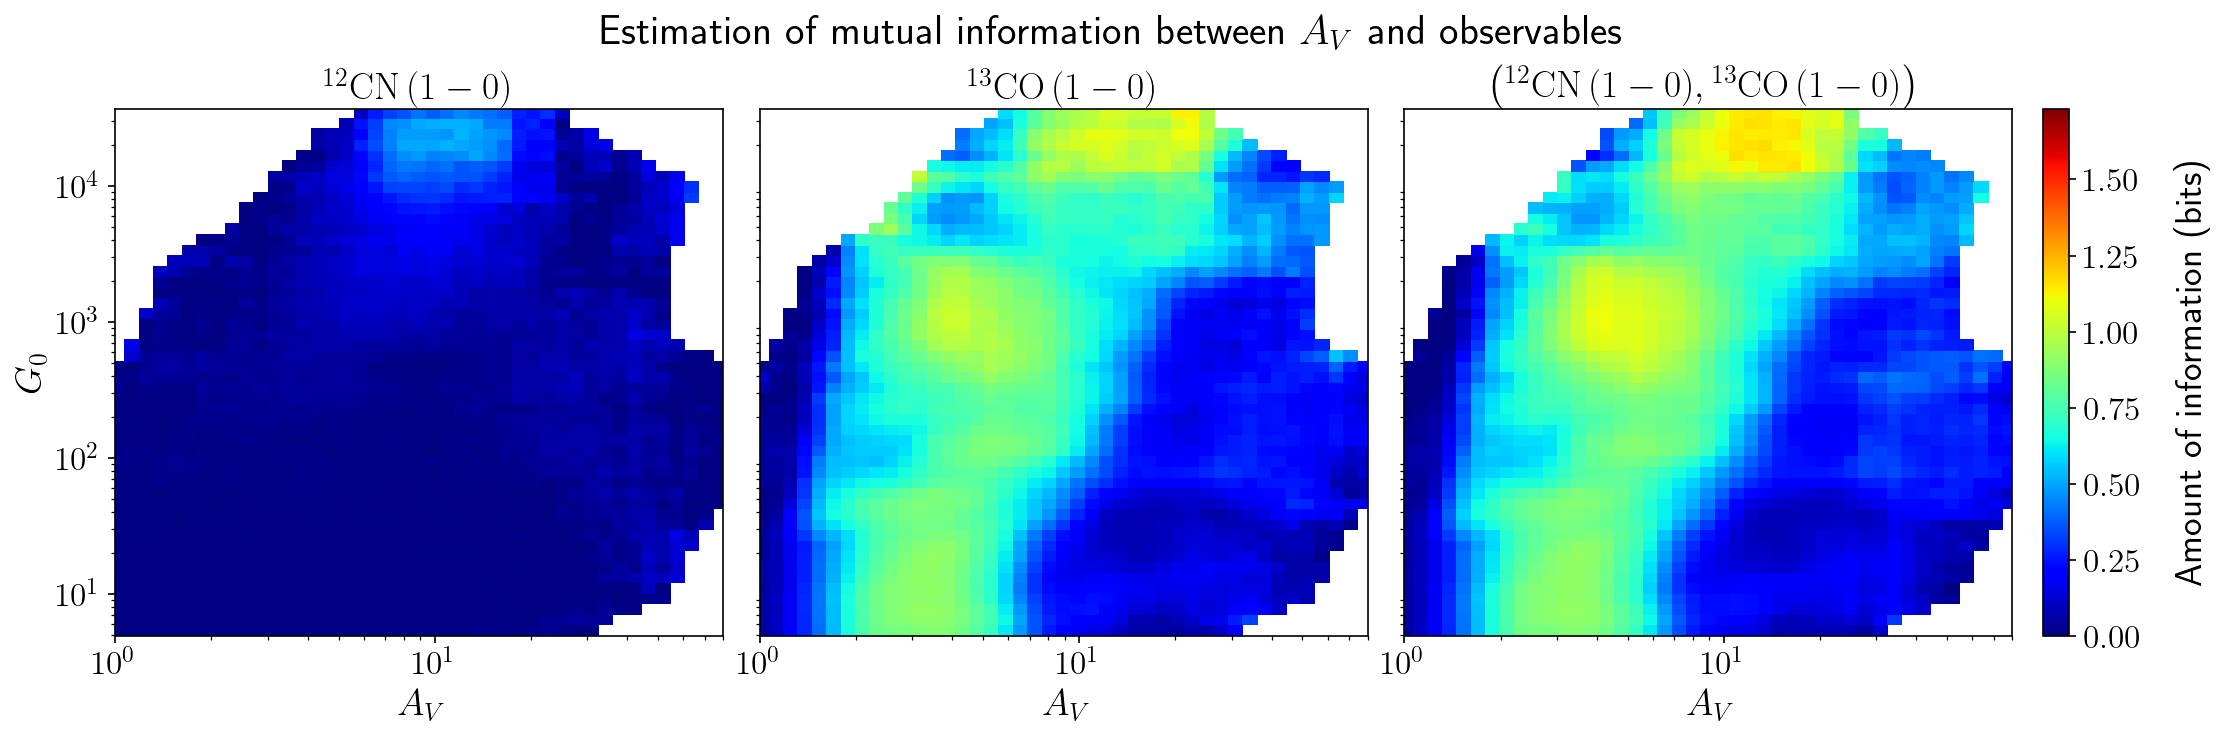
\includegraphics[width=0.95\linewidth]{../mi/av__12cn10_13co10_mi.png}
        \vfill
        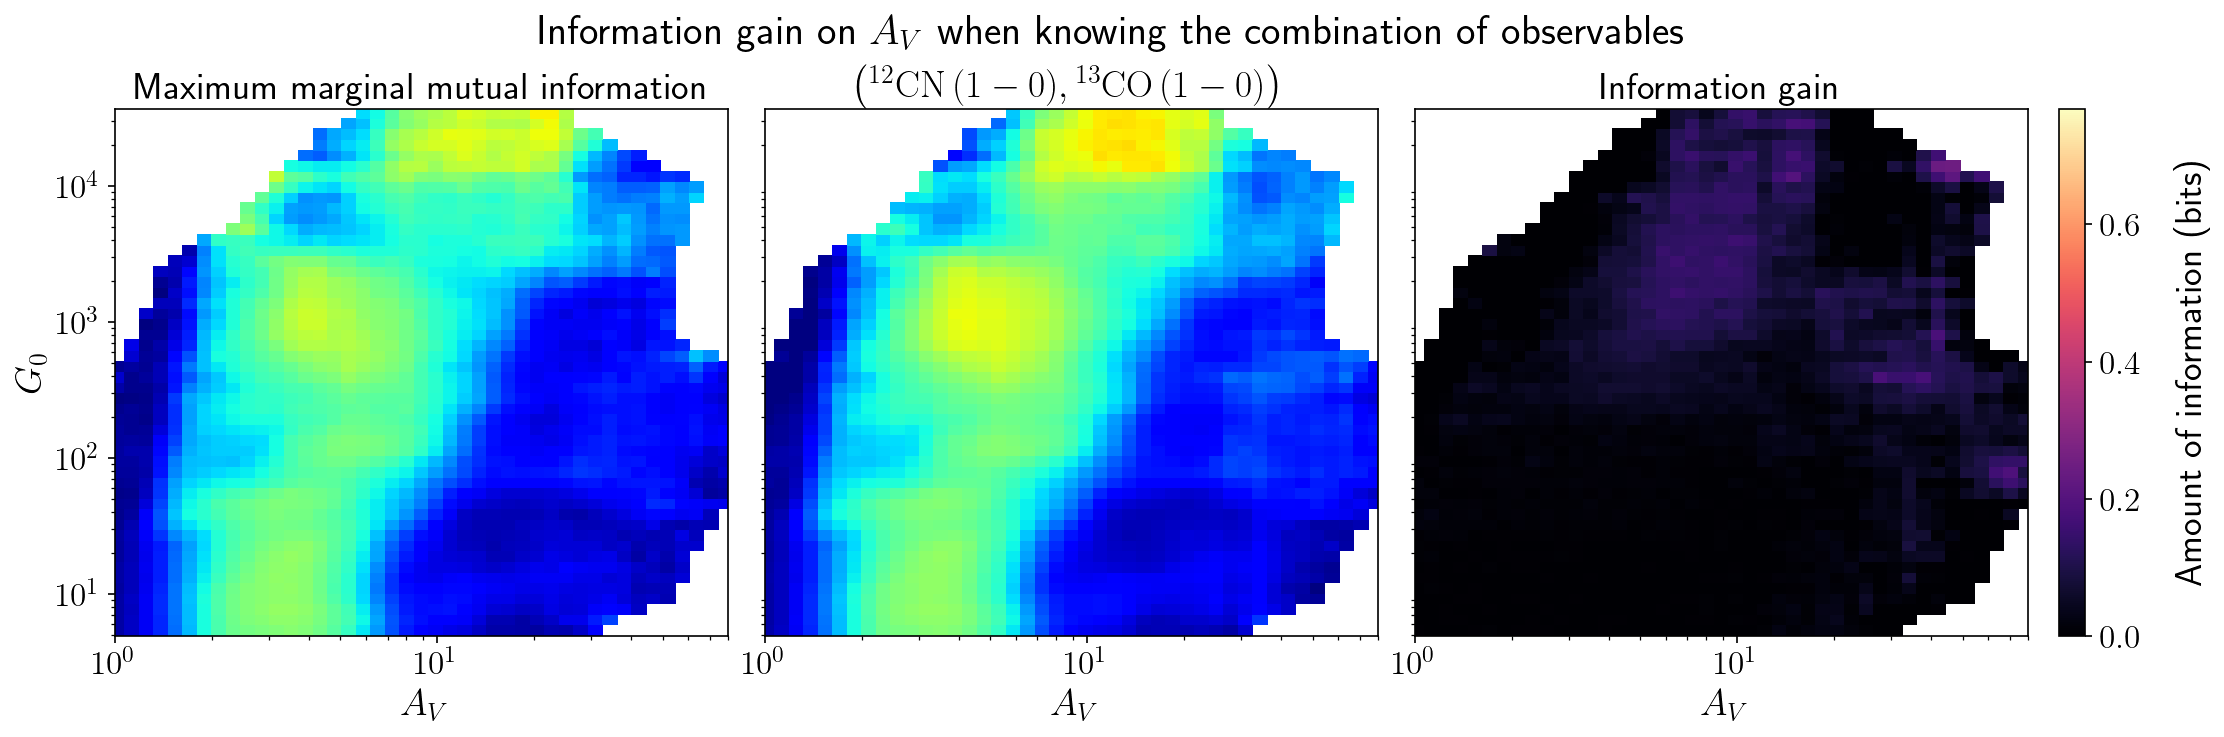
\includegraphics[width=0.95\linewidth]{../mi/av__12cn10_13co10_mi_gain.png}
    \end{figure}
\end{frame}

\begin{frame}{Informativity on $A_V$ of $\left(\mathrm{^{12}CO\,(1-0)},\mathrm{^{13}CO\,(1-0)}\right)$}
    \begin{figure}
        \centering
        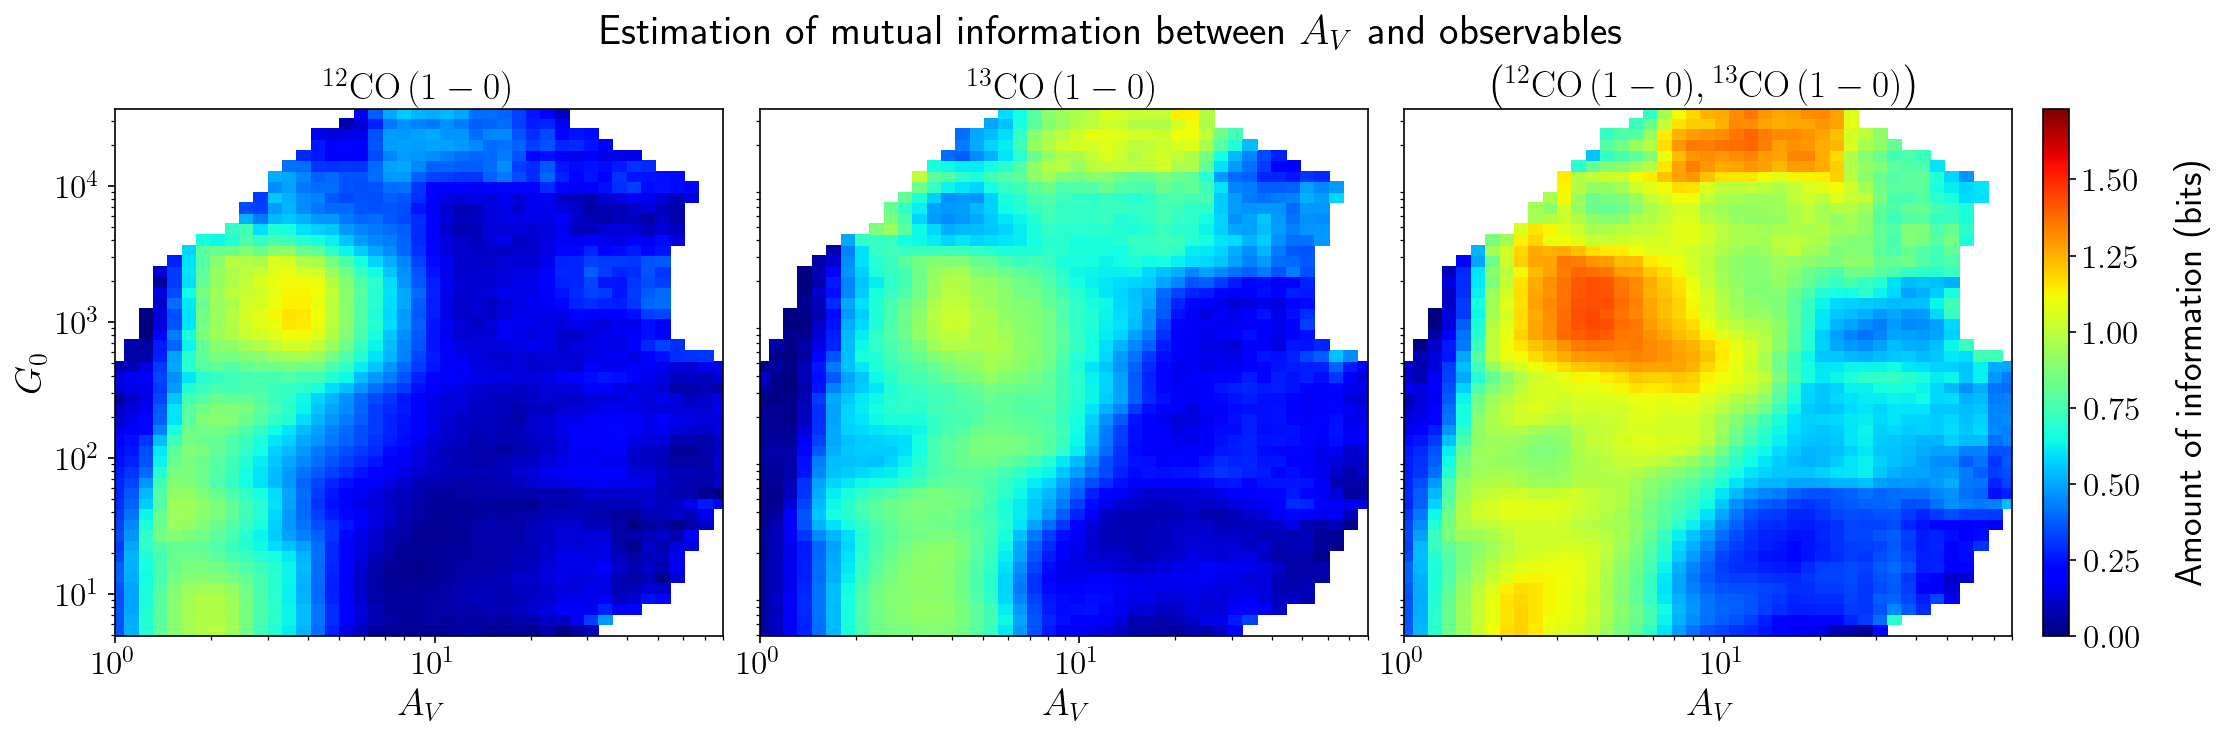
\includegraphics[width=0.95\linewidth]{../mi/av__12co10_13co10_mi.png}
        \vfill
        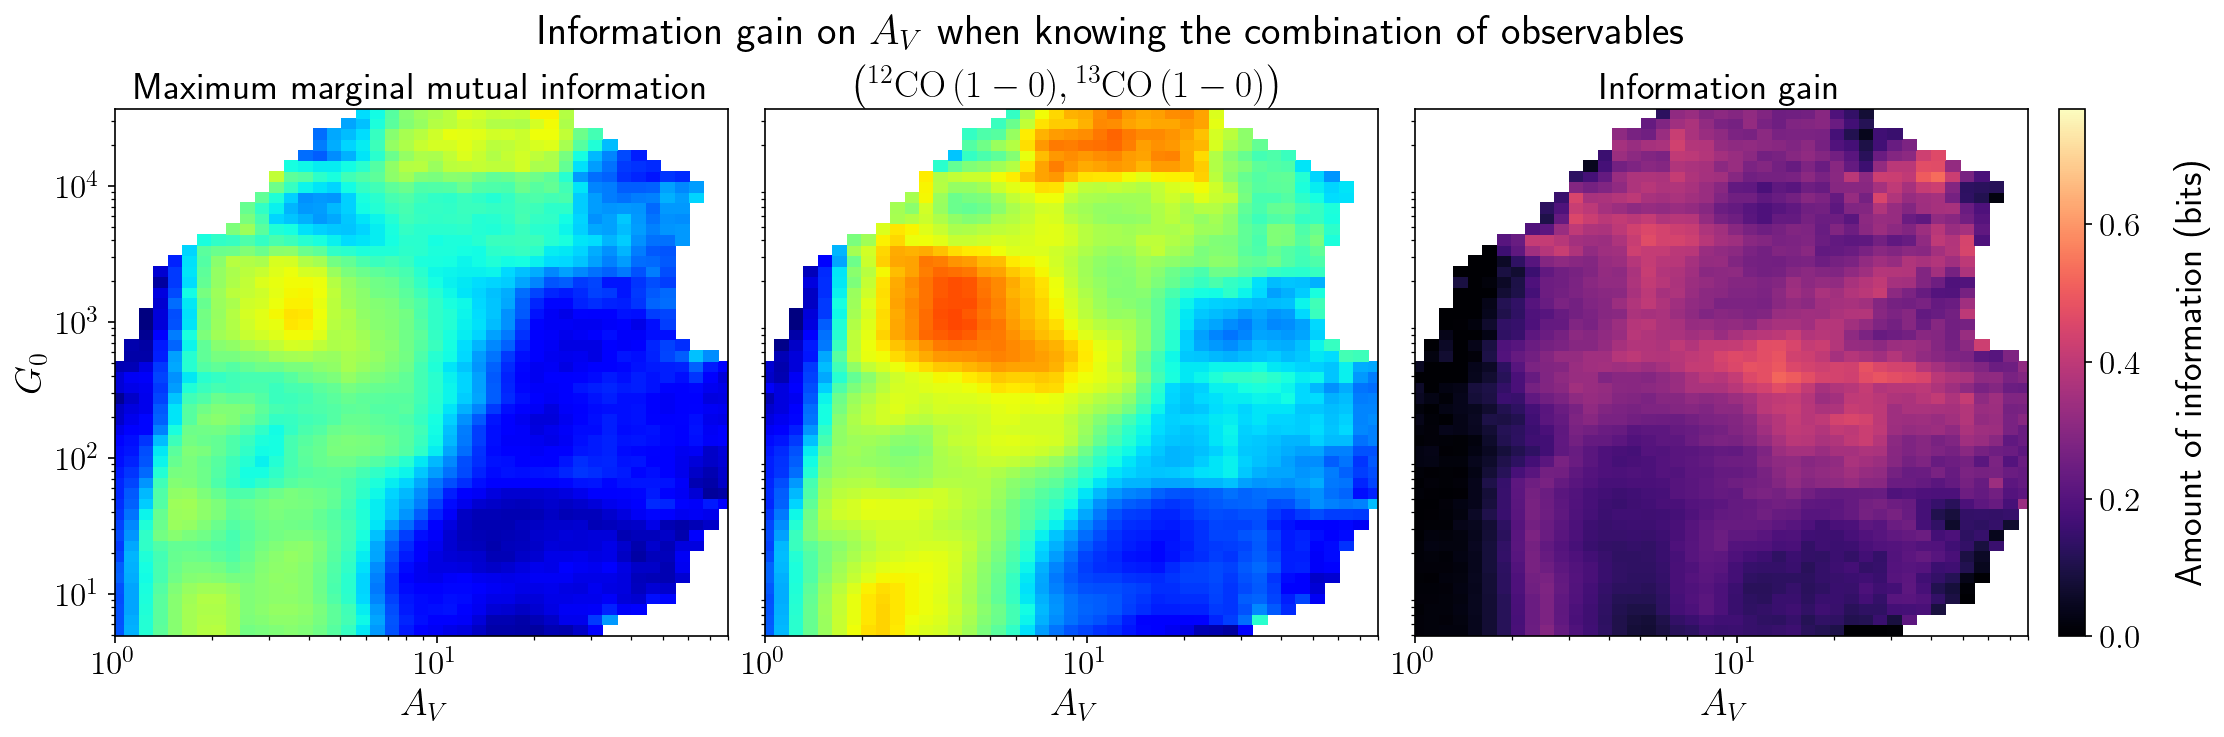
\includegraphics[width=0.95\linewidth]{../mi/av__12co10_13co10_mi_gain.png}
    \end{figure}
\end{frame}

\begin{frame}{Informativity on $A_V$ of $\left(\mathrm{^{12}CS\,(2-1)},\mathrm{^{13}CO\,(1-0)}\right)$}
    \begin{figure}
        \centering
        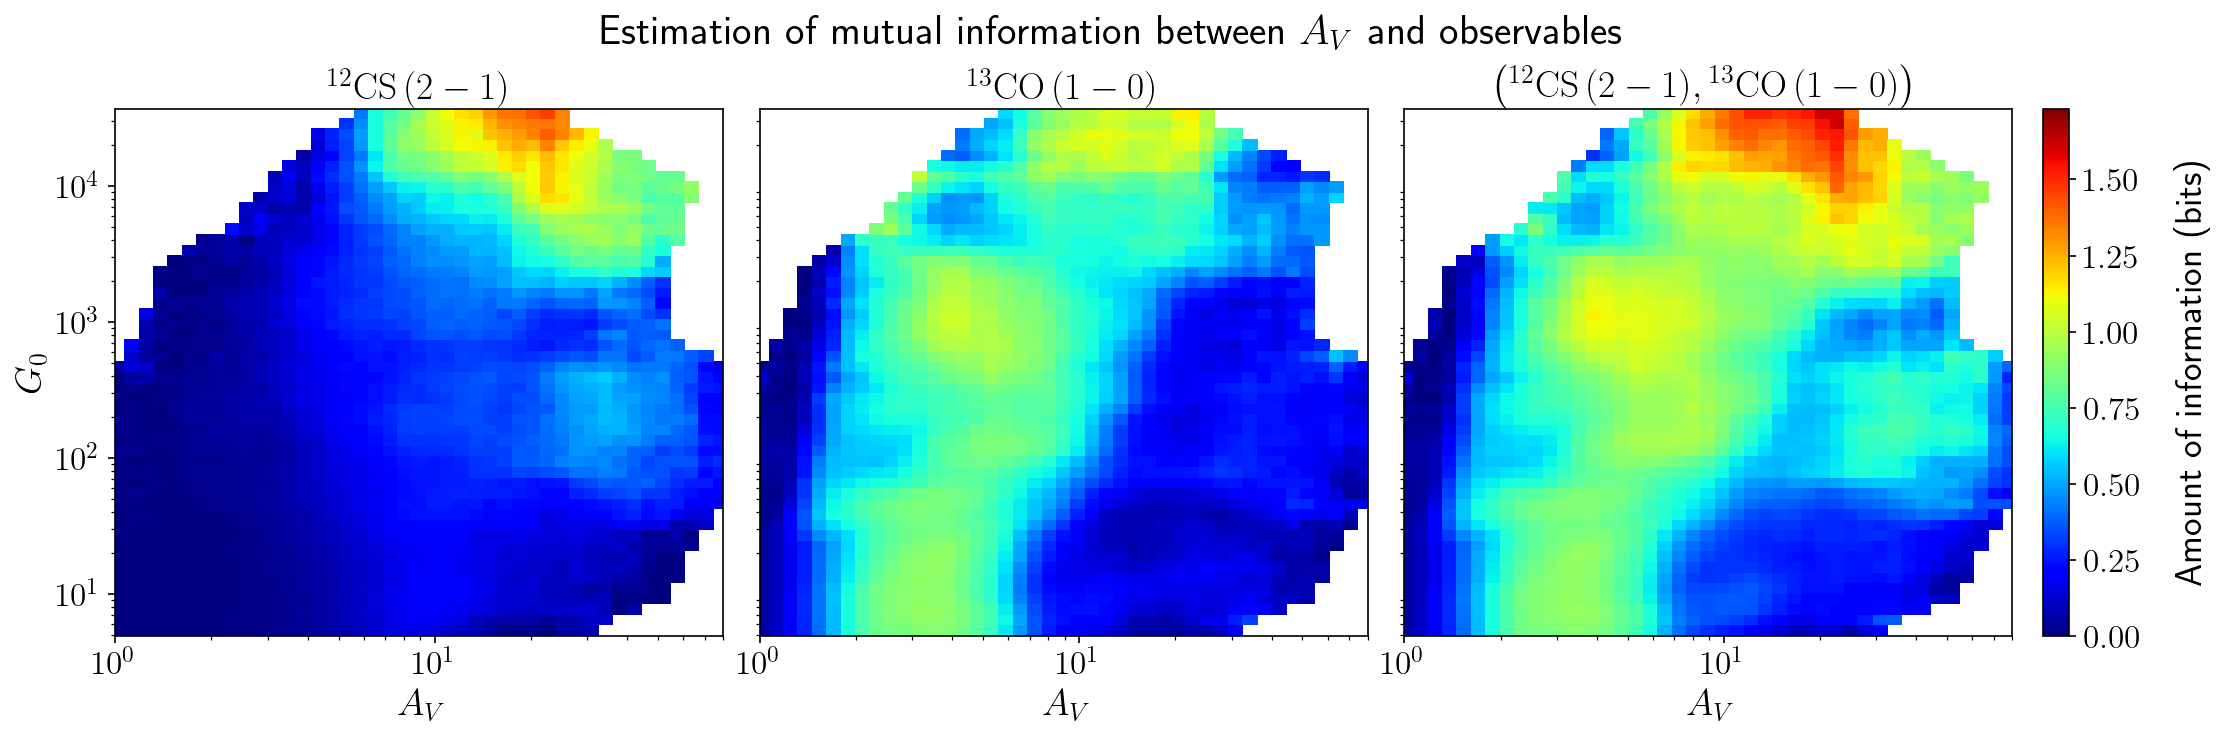
\includegraphics[width=0.95\linewidth]{../mi/av__12cs21_13co10_mi.png}
        \vfill
        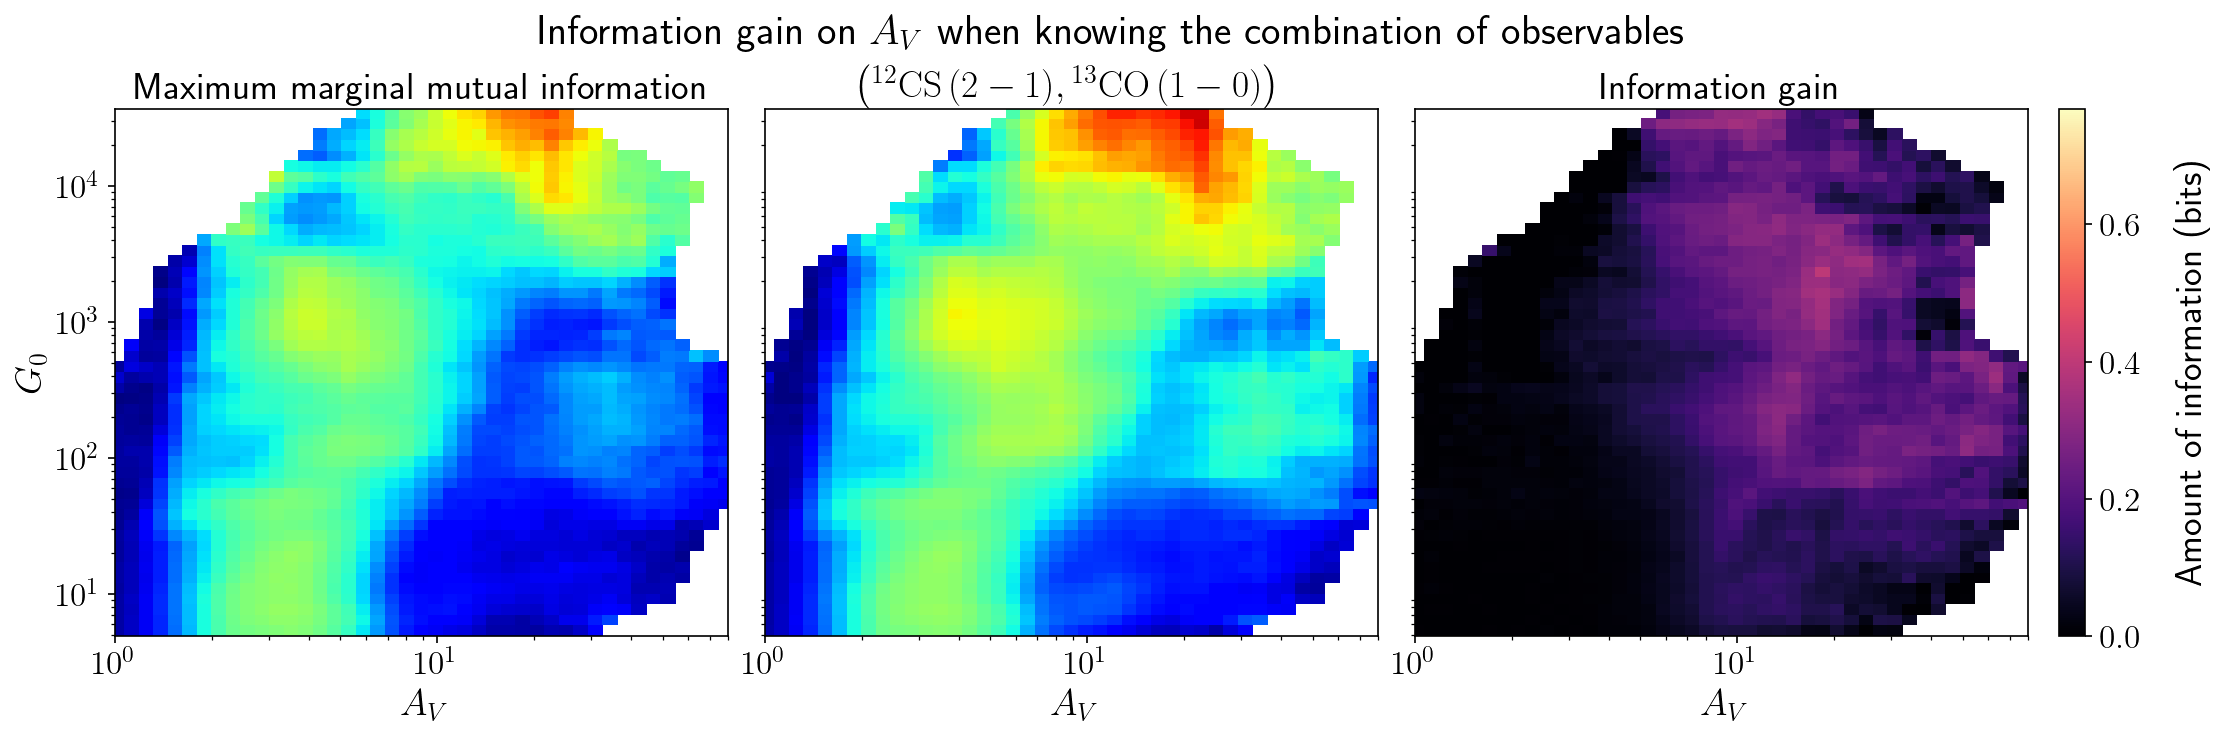
\includegraphics[width=0.95\linewidth]{../mi/av__12cs21_13co10_mi_gain.png}
    \end{figure}
\end{frame}

\begin{frame}{Informativity on $A_V$ of $\left(\mathrm{^{13}CO\,(1-0)},\mathrm{^{32}SO\,(2-1)}\right)$}
    \begin{figure}
        \centering
        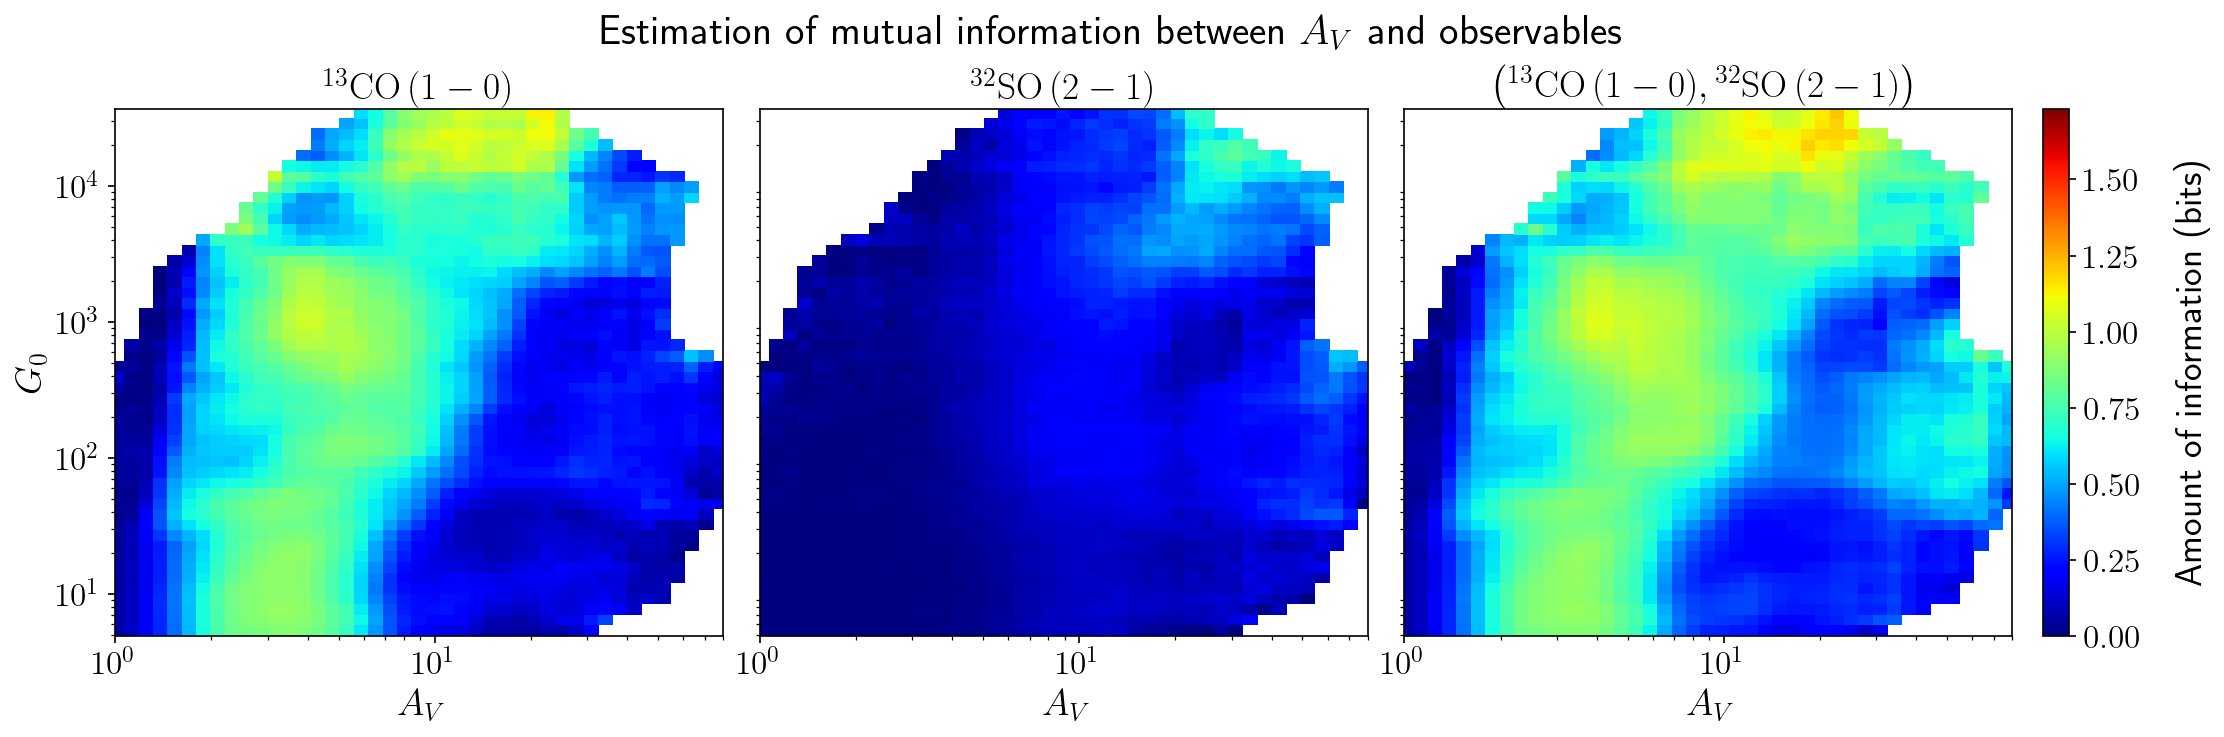
\includegraphics[width=0.95\linewidth]{../mi/av__13co10_32so21_mi.png}
        \vfill
        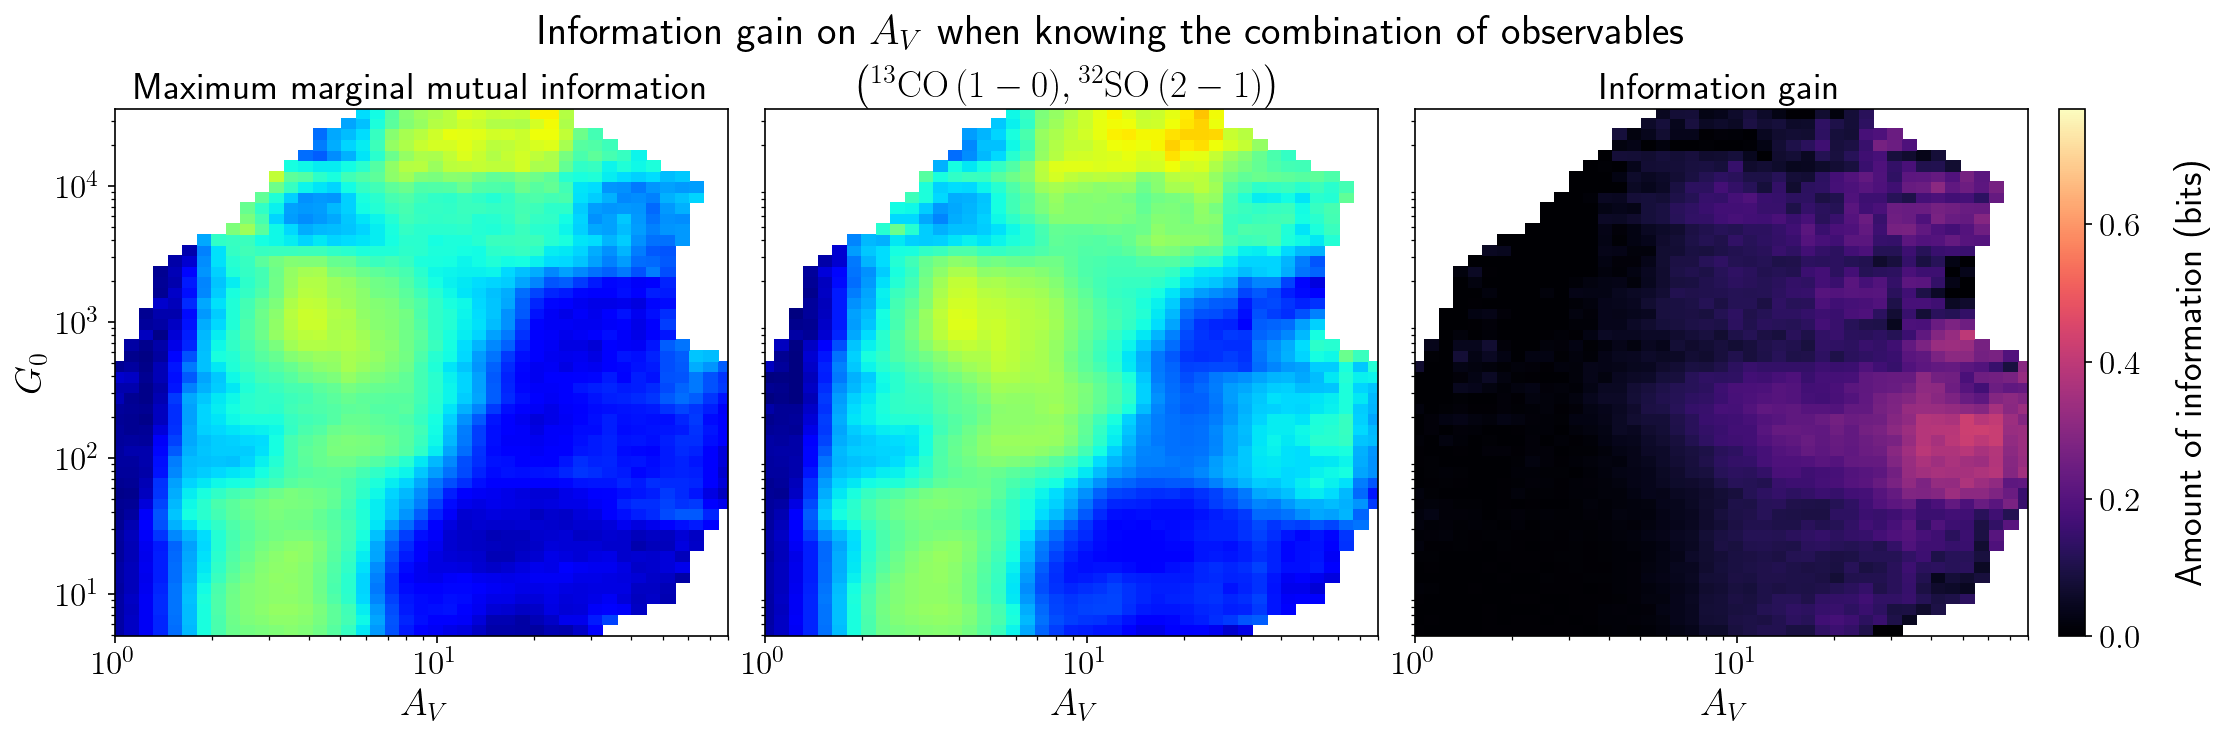
\includegraphics[width=0.95\linewidth]{../mi/av__13co10_32so21_mi_gain.png}
    \end{figure}
\end{frame}

\begin{frame}{Informativity on $A_V$ of $\left(\mathrm{^{13}CO\,(1-0)},\mathrm{C^{18}O\,(1-0)}\right)$}
    \begin{figure}
        \centering
        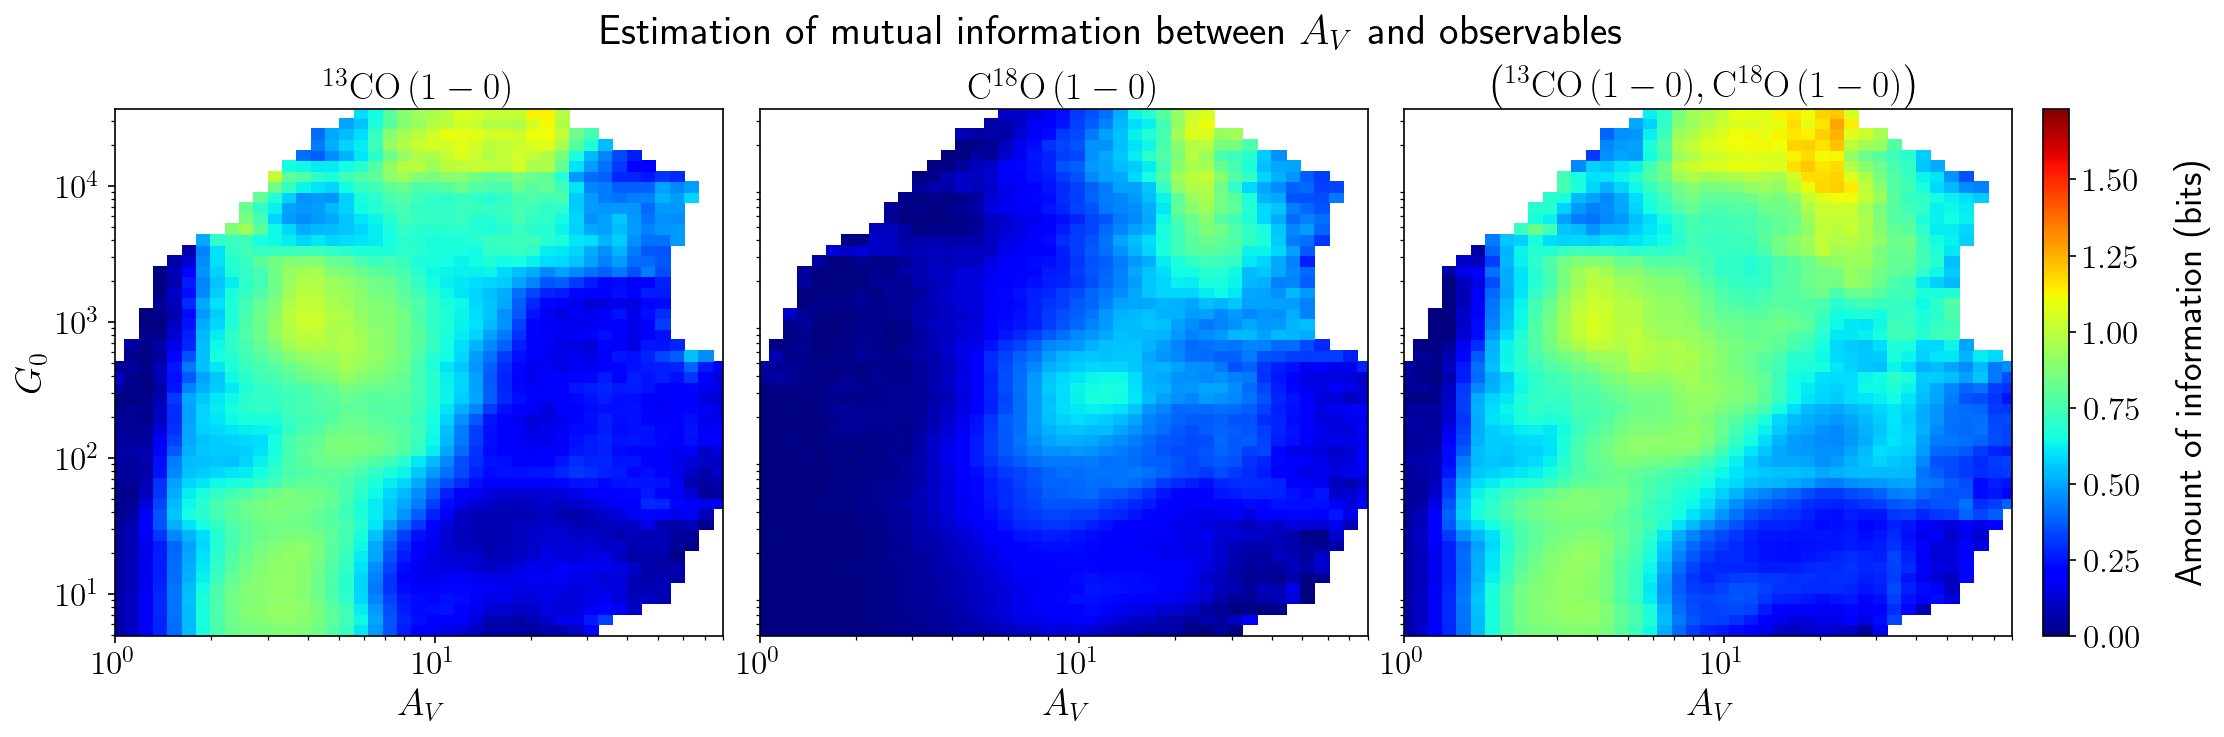
\includegraphics[width=0.95\linewidth]{../mi/av__13co10_c18o10_mi.png}
        \vfill
        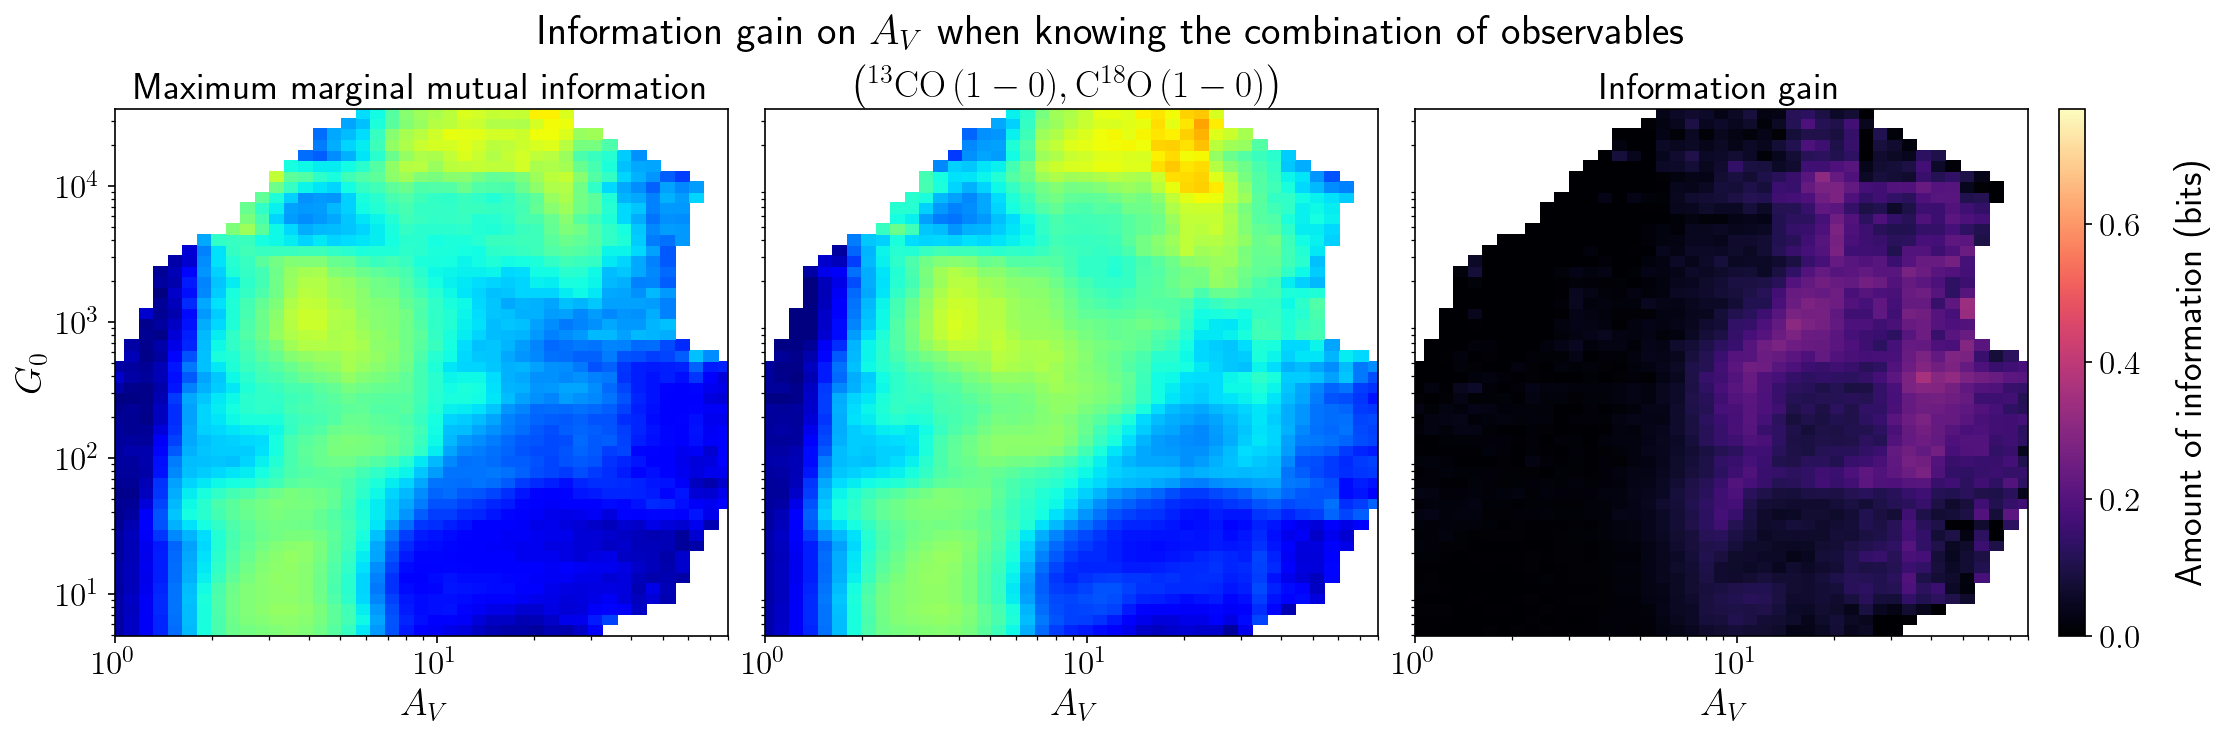
\includegraphics[width=0.95\linewidth]{../mi/av__13co10_c18o10_mi_gain.png}
    \end{figure}
\end{frame}

\begin{frame}{Informativity on $A_V$ of $\left(\mathrm{^{13}CO\,(1-0)},\mathrm{CCH\,(1-0)}\right)$}
    \begin{figure}
        \centering
        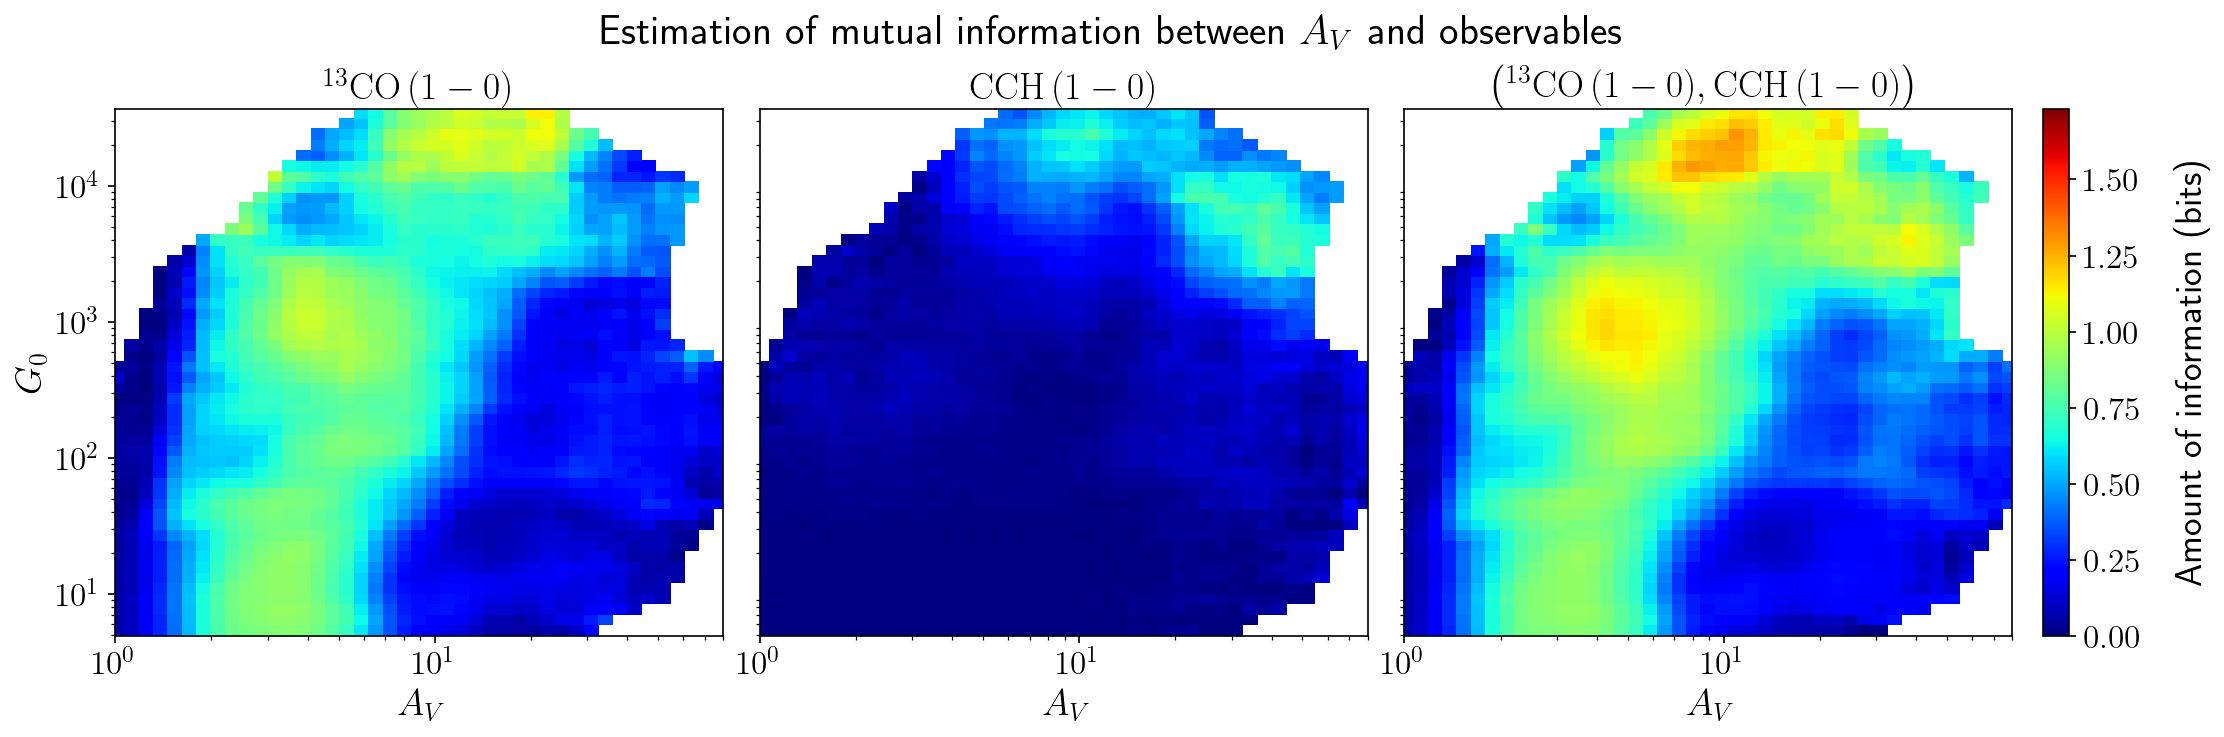
\includegraphics[width=0.95\linewidth]{../mi/av__13co10_cch10_mi.png}
        \vfill
        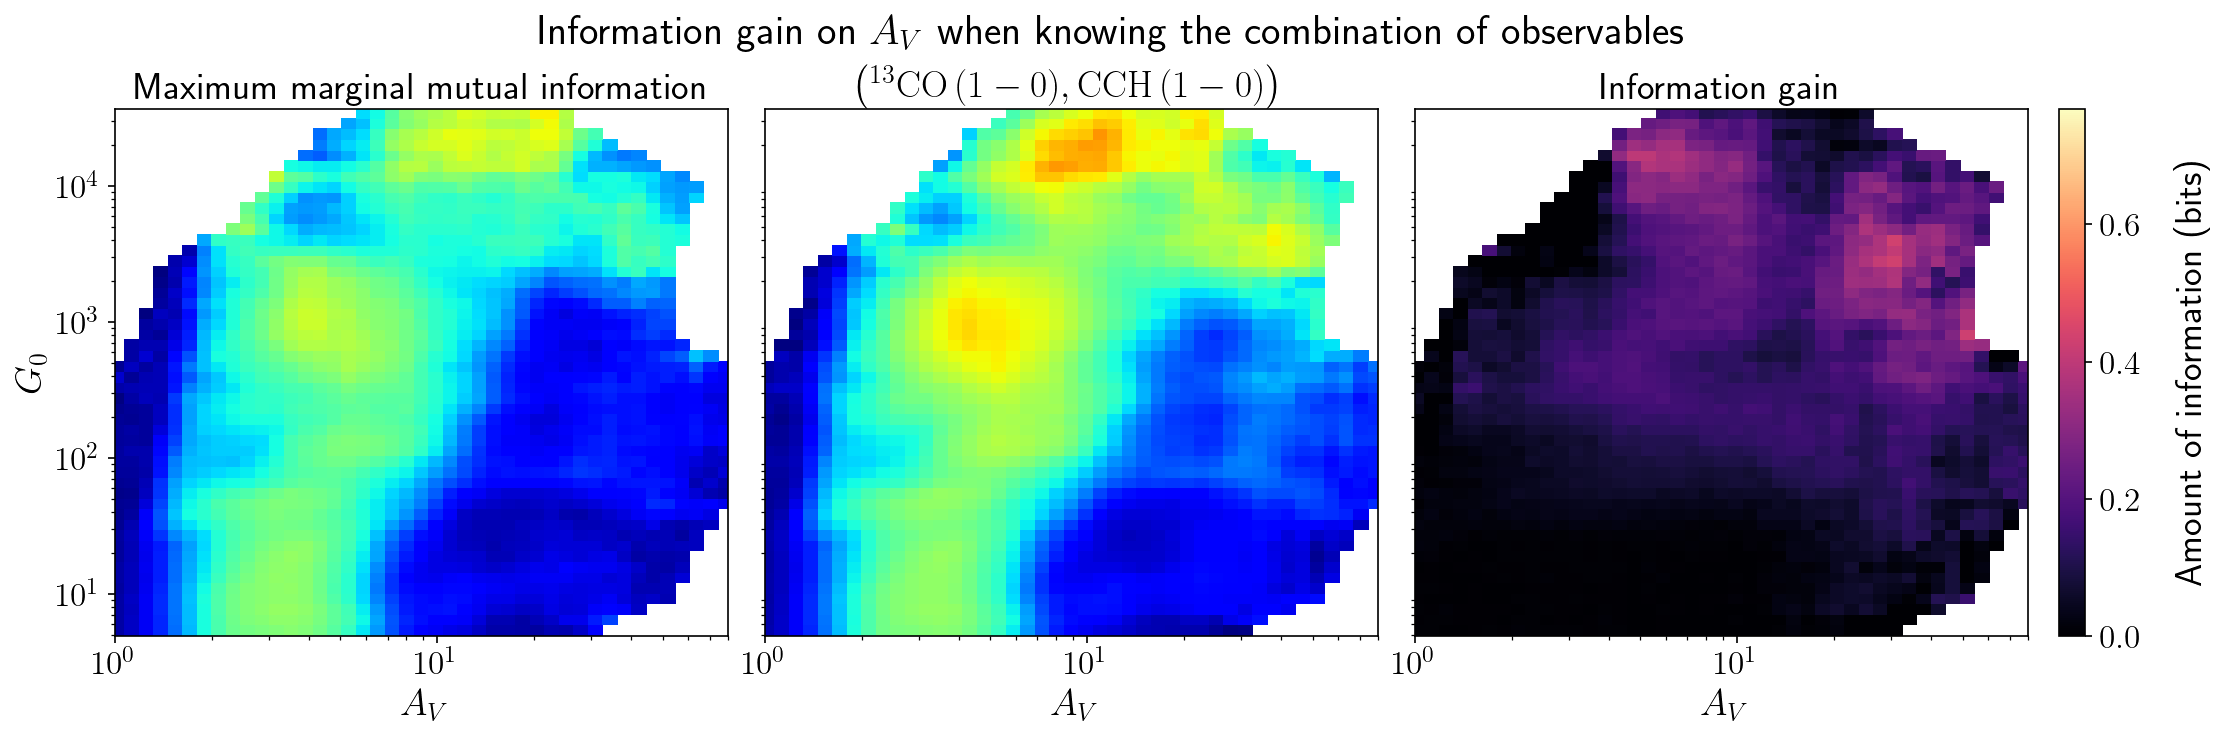
\includegraphics[width=0.95\linewidth]{../mi/av__13co10_cch10_mi_gain.png}
    \end{figure}
\end{frame}

\begin{frame}{Informativity on $A_V$ of $\left(\mathrm{^{13}CO\,(1-0)},\mathrm{H_2CO}\right)$}
    \begin{figure}
        \centering
        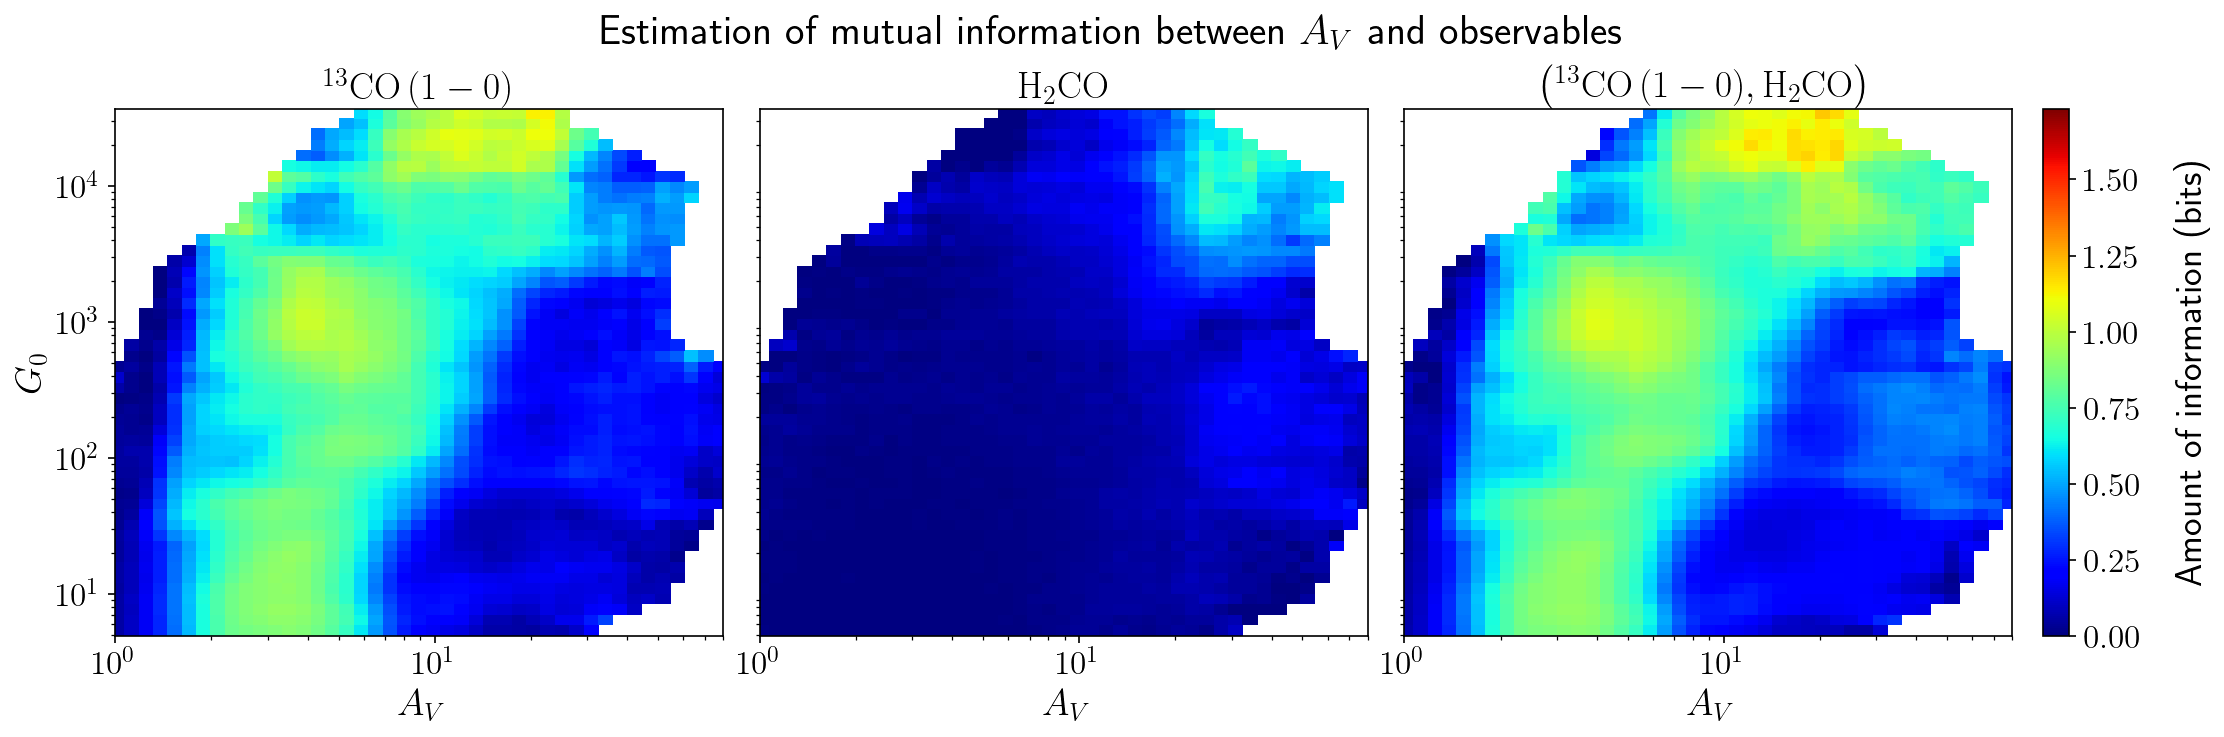
\includegraphics[width=0.95\linewidth]{../mi/av__13co10_h2co_mi.png}
        \vfill
        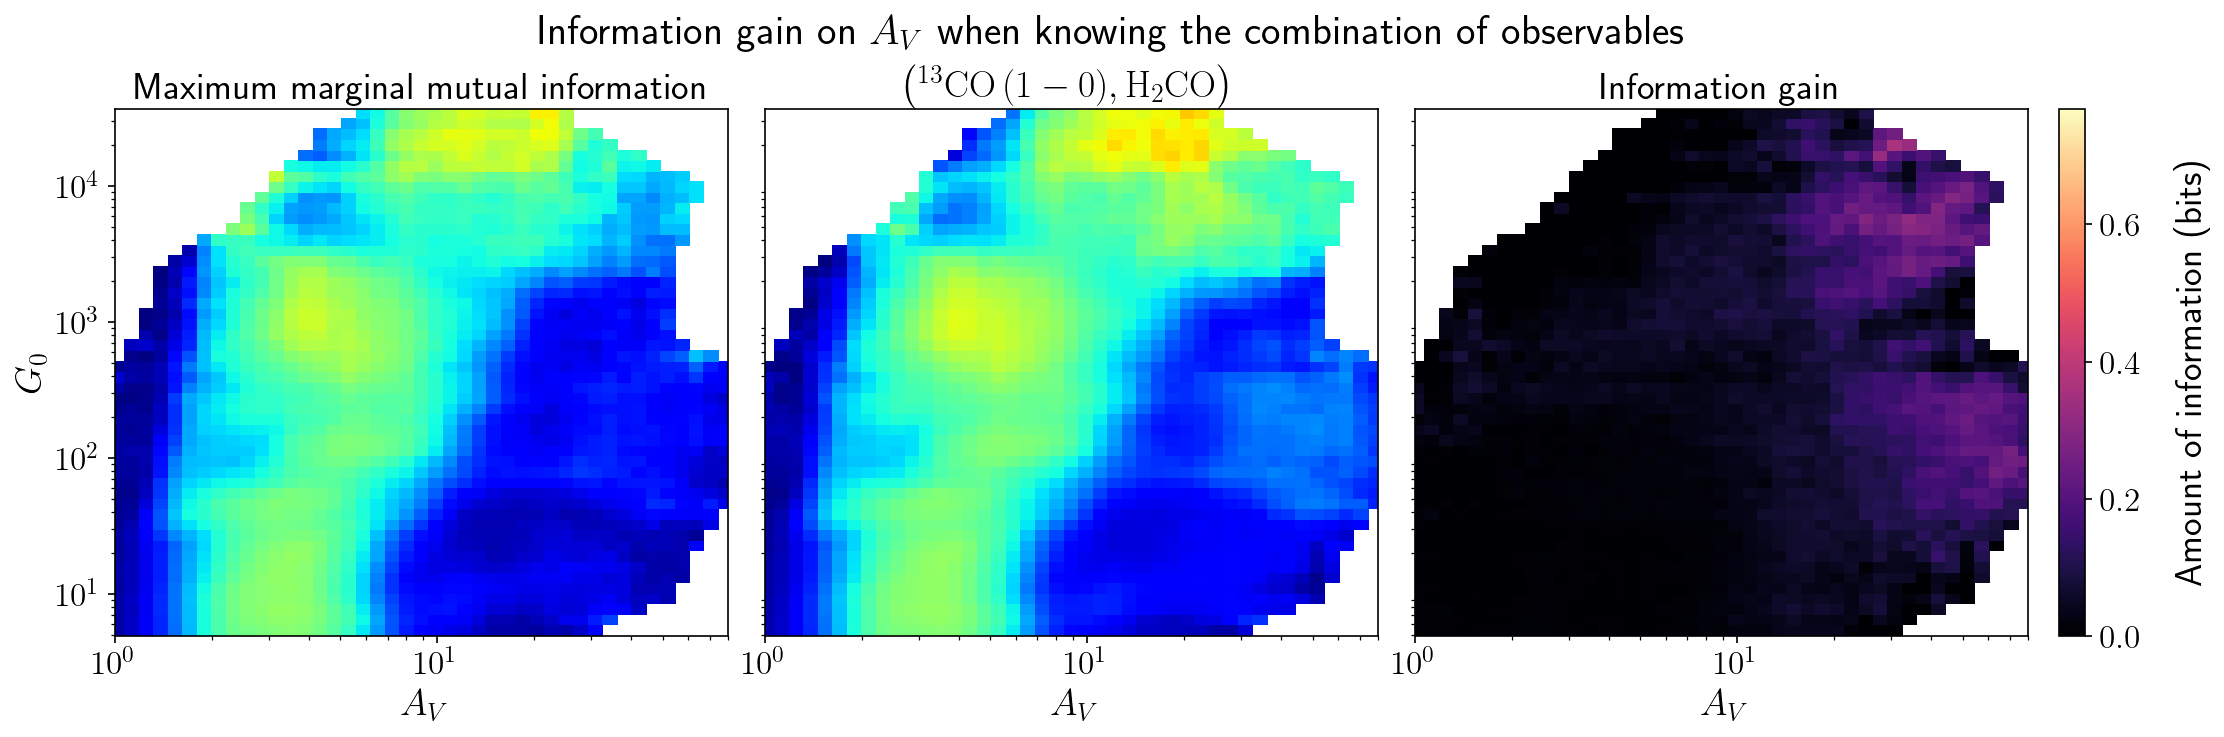
\includegraphics[width=0.95\linewidth]{../mi/av__13co10_h2co_mi_gain.png}
    \end{figure}
\end{frame}

\begin{frame}{Informativity on $A_V$ of $\left(\mathrm{^{13}CO\,(1-0)},\mathrm{HCN\,(1-0)}\right)$}
    \begin{figure}
        \centering
        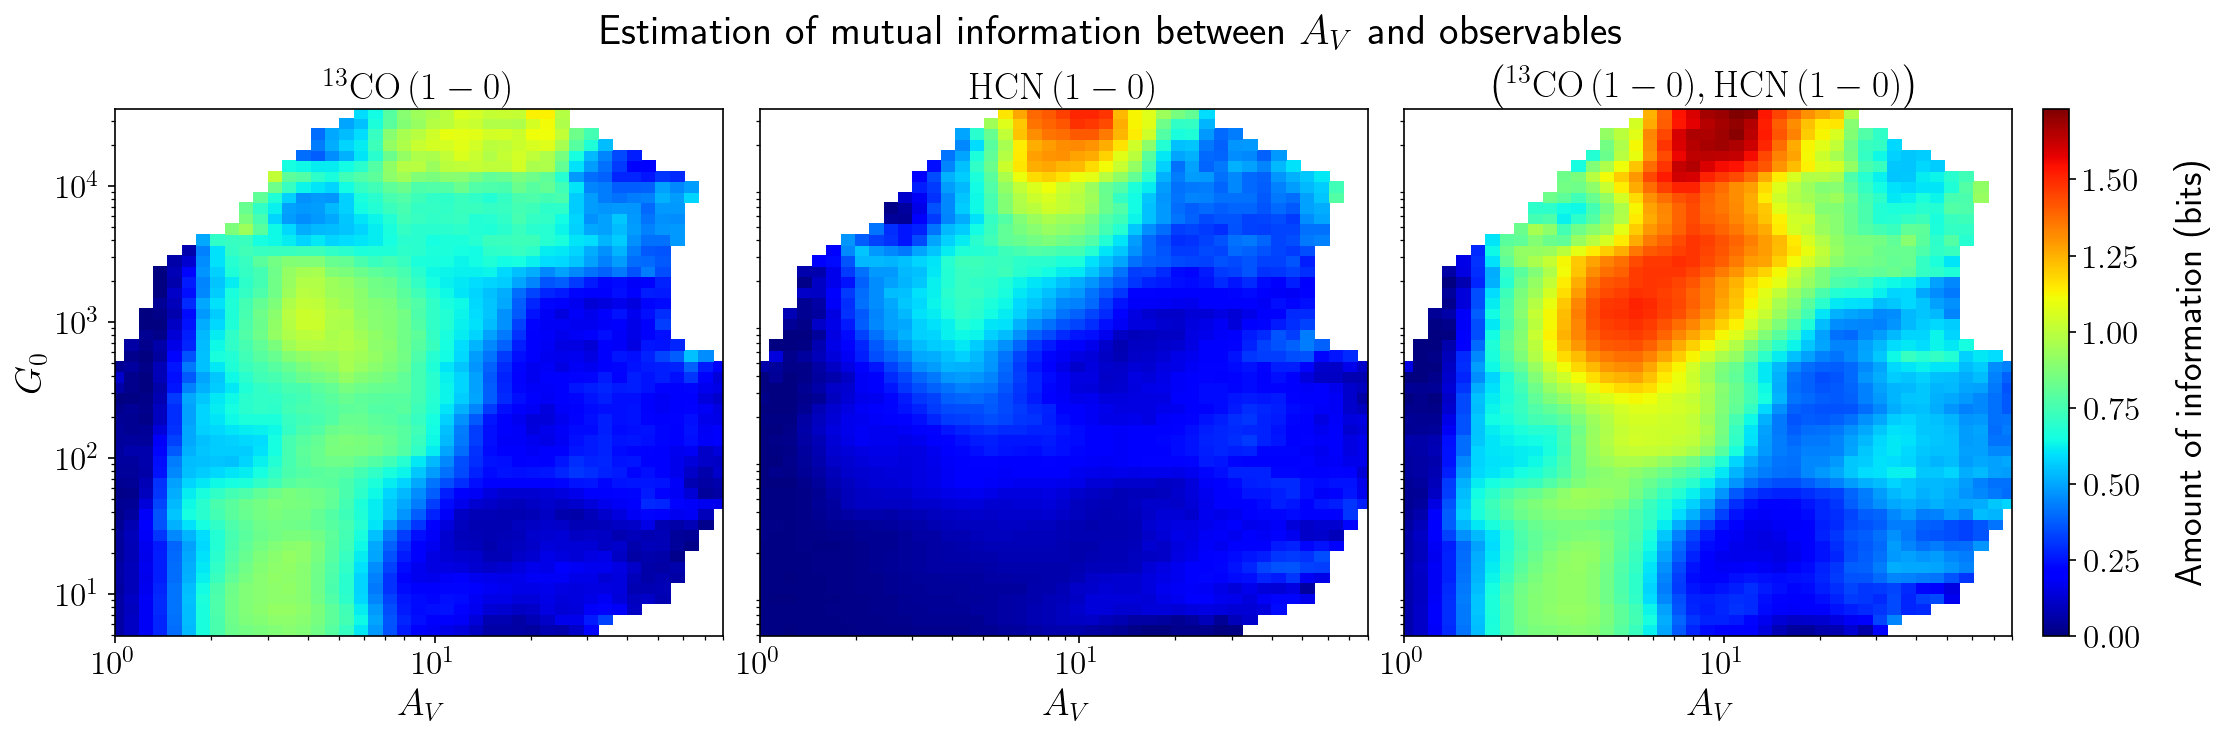
\includegraphics[width=0.95\linewidth]{../mi/av__13co10_hcn10_mi.png}
        \vfill
        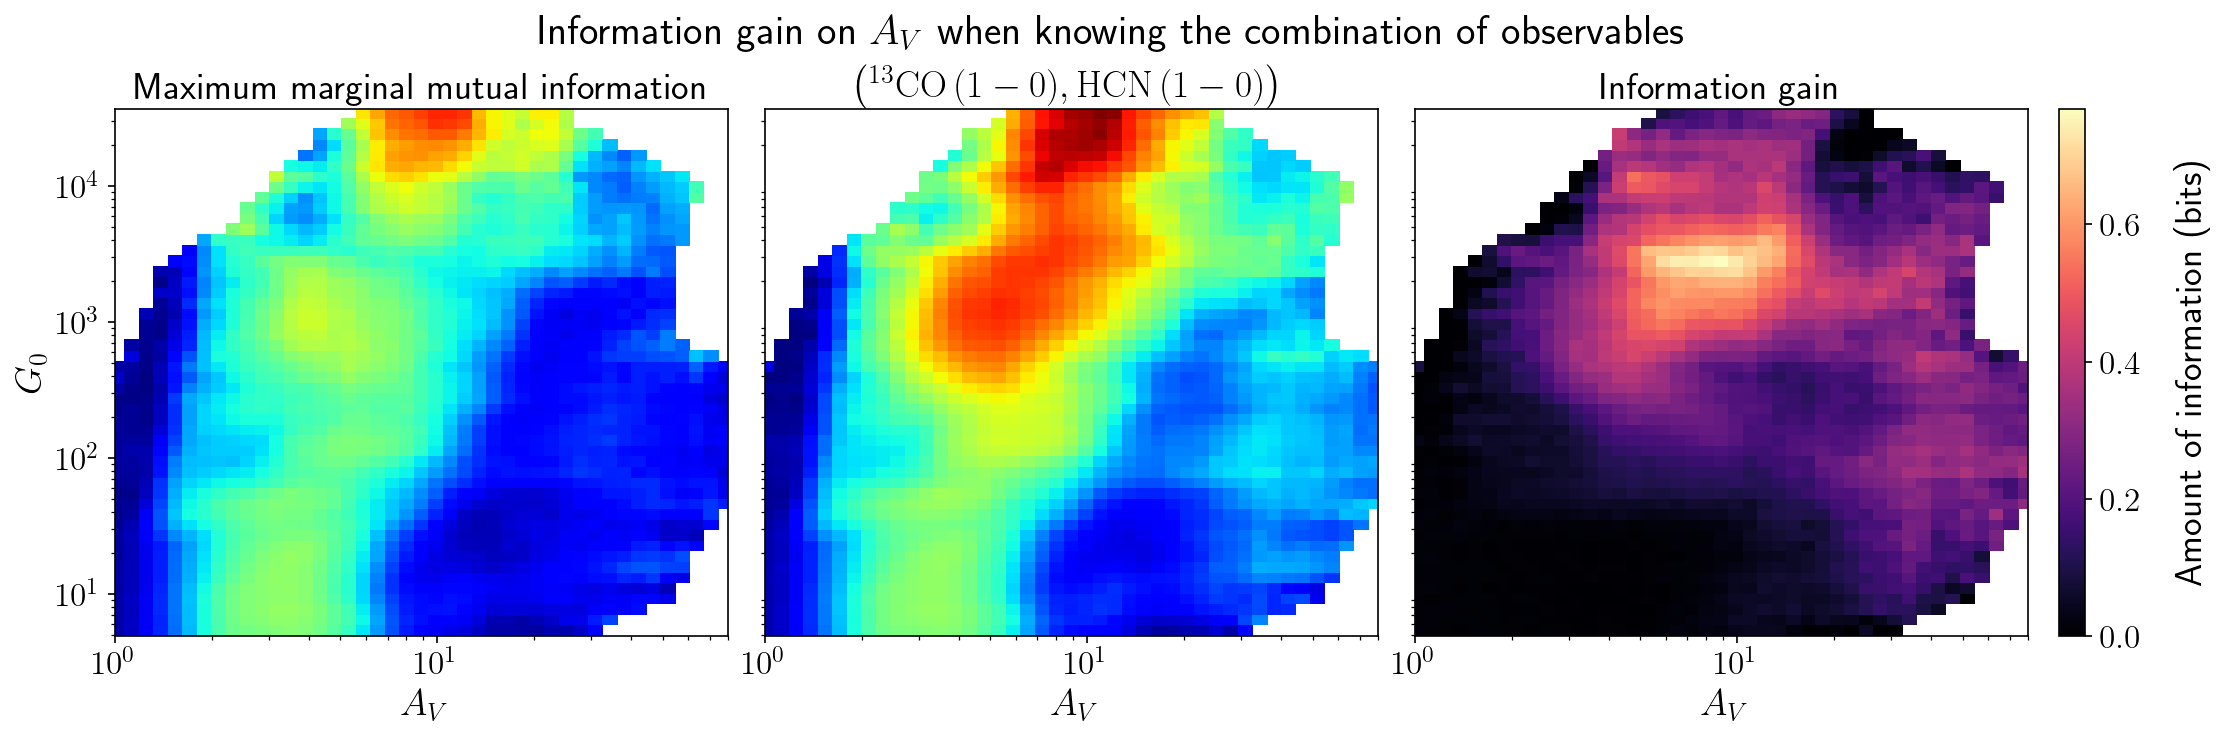
\includegraphics[width=0.95\linewidth]{../mi/av__13co10_hcn10_mi_gain.png}
    \end{figure}
\end{frame}

\begin{frame}{Informativity on $A_V$ of $\left(\mathrm{^{13}CO\,(1-0)},\mathrm{HCO^+\,(1-0)}\right)$}
    \begin{figure}
        \centering
        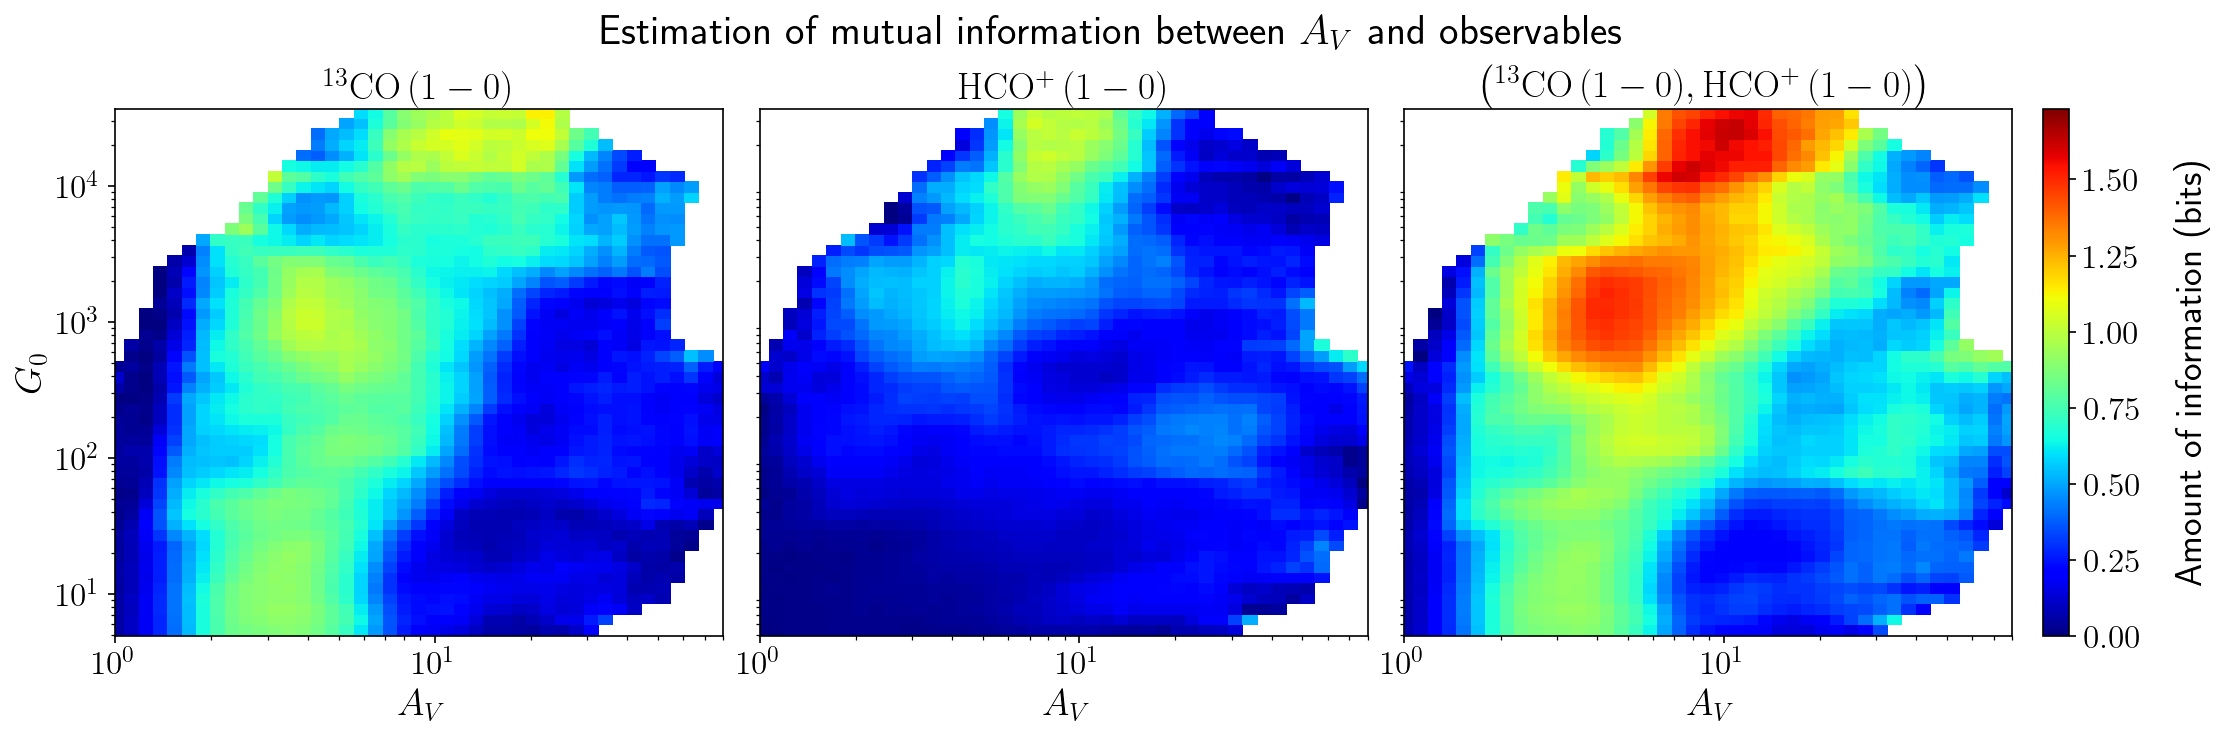
\includegraphics[width=0.95\linewidth]{../mi/av__13co10_hcop10_mi.png}
        \vfill
        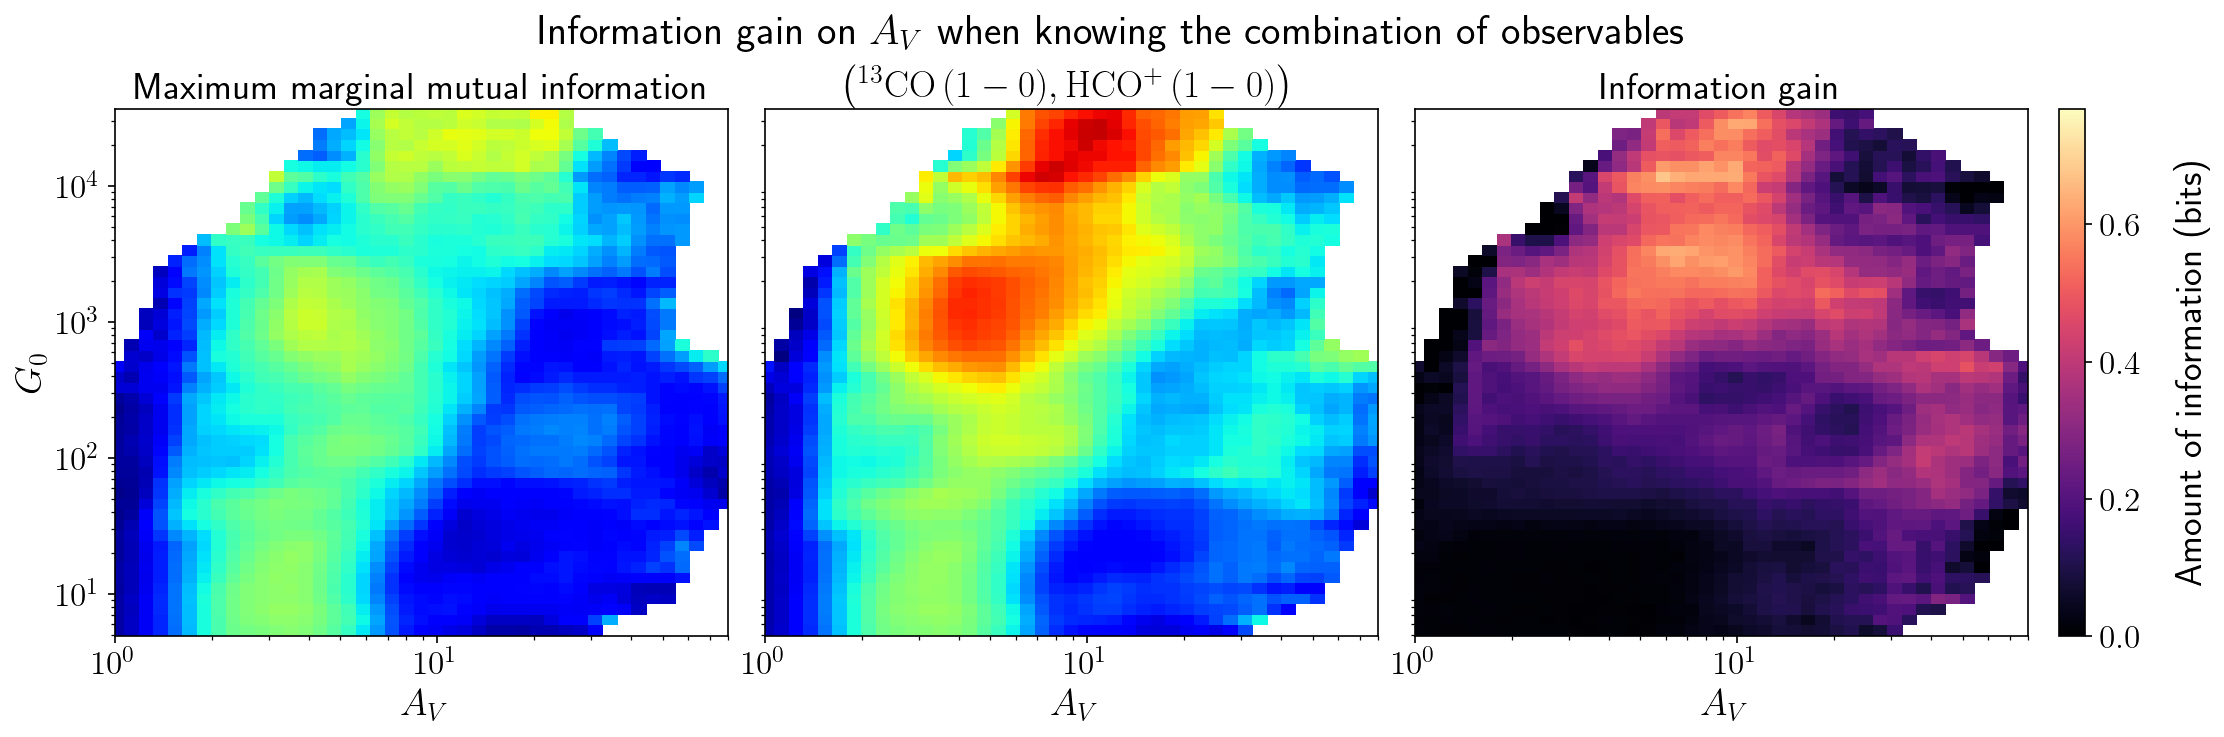
\includegraphics[width=0.95\linewidth]{../mi/av__13co10_hcop10_mi_gain.png}
    \end{figure}
\end{frame}

\begin{frame}{Informativity on $A_V$ of $\left(\mathrm{^{13}CO\,(1-0)},\mathrm{HNC\,(1-0)}\right)$}
    \begin{figure}
        \centering
        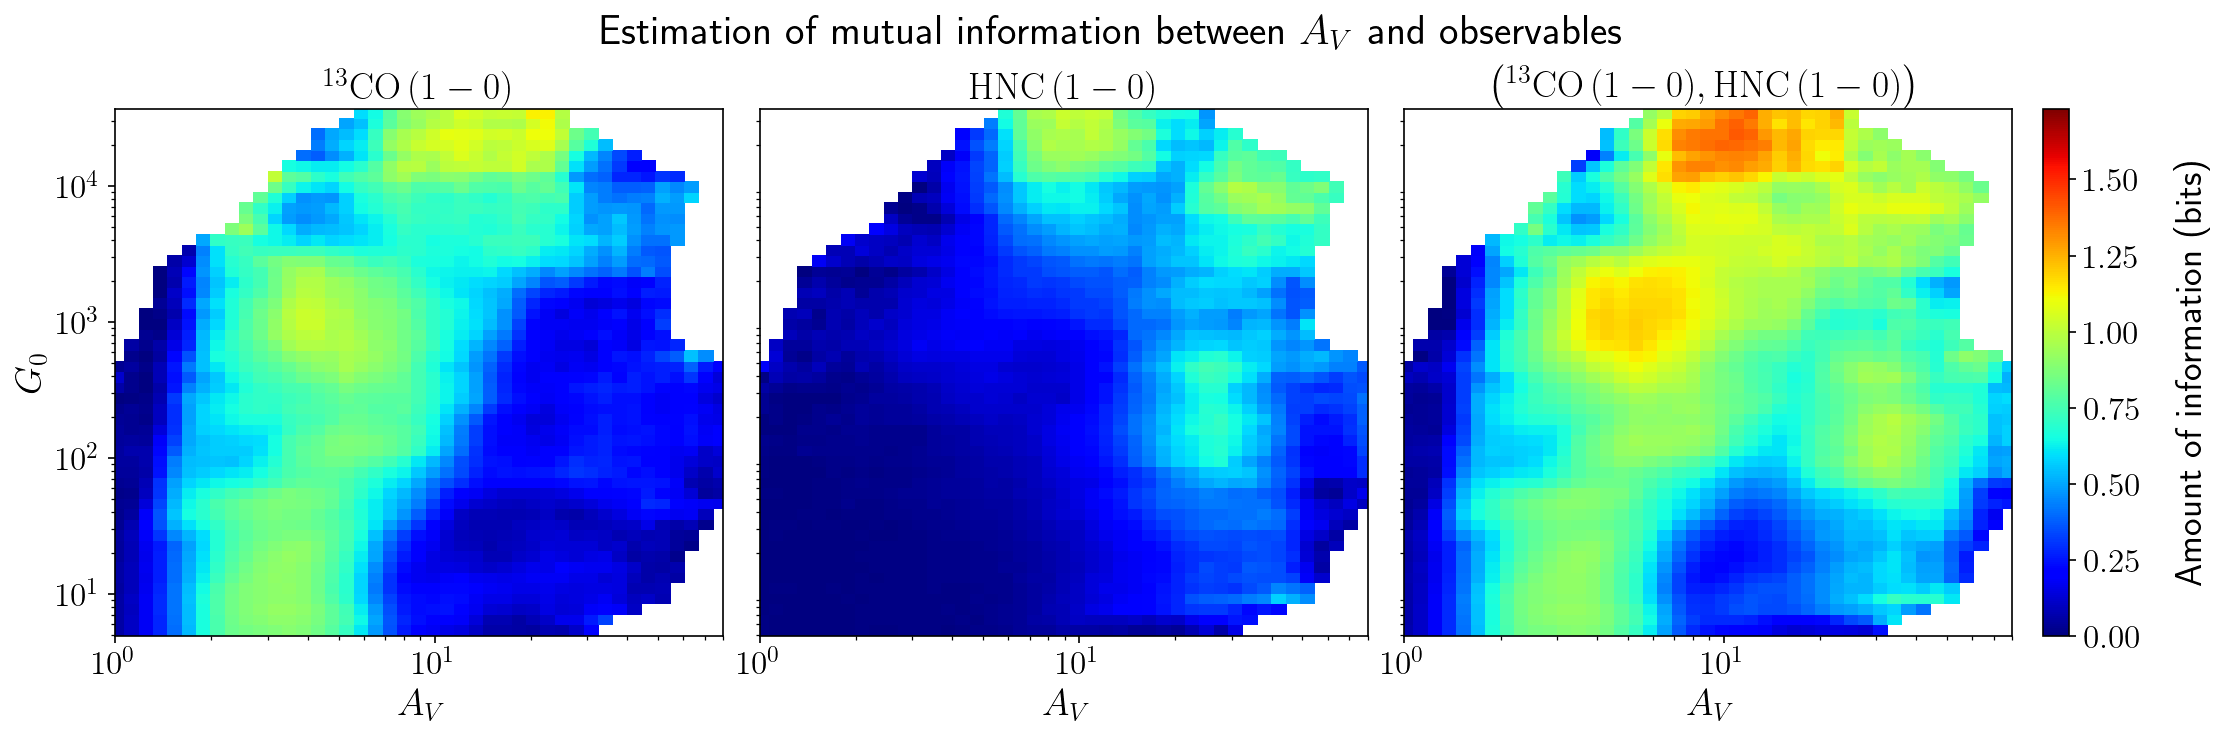
\includegraphics[width=0.95\linewidth]{../mi/av__13co10_hnc10_mi.png}
        \vfill
        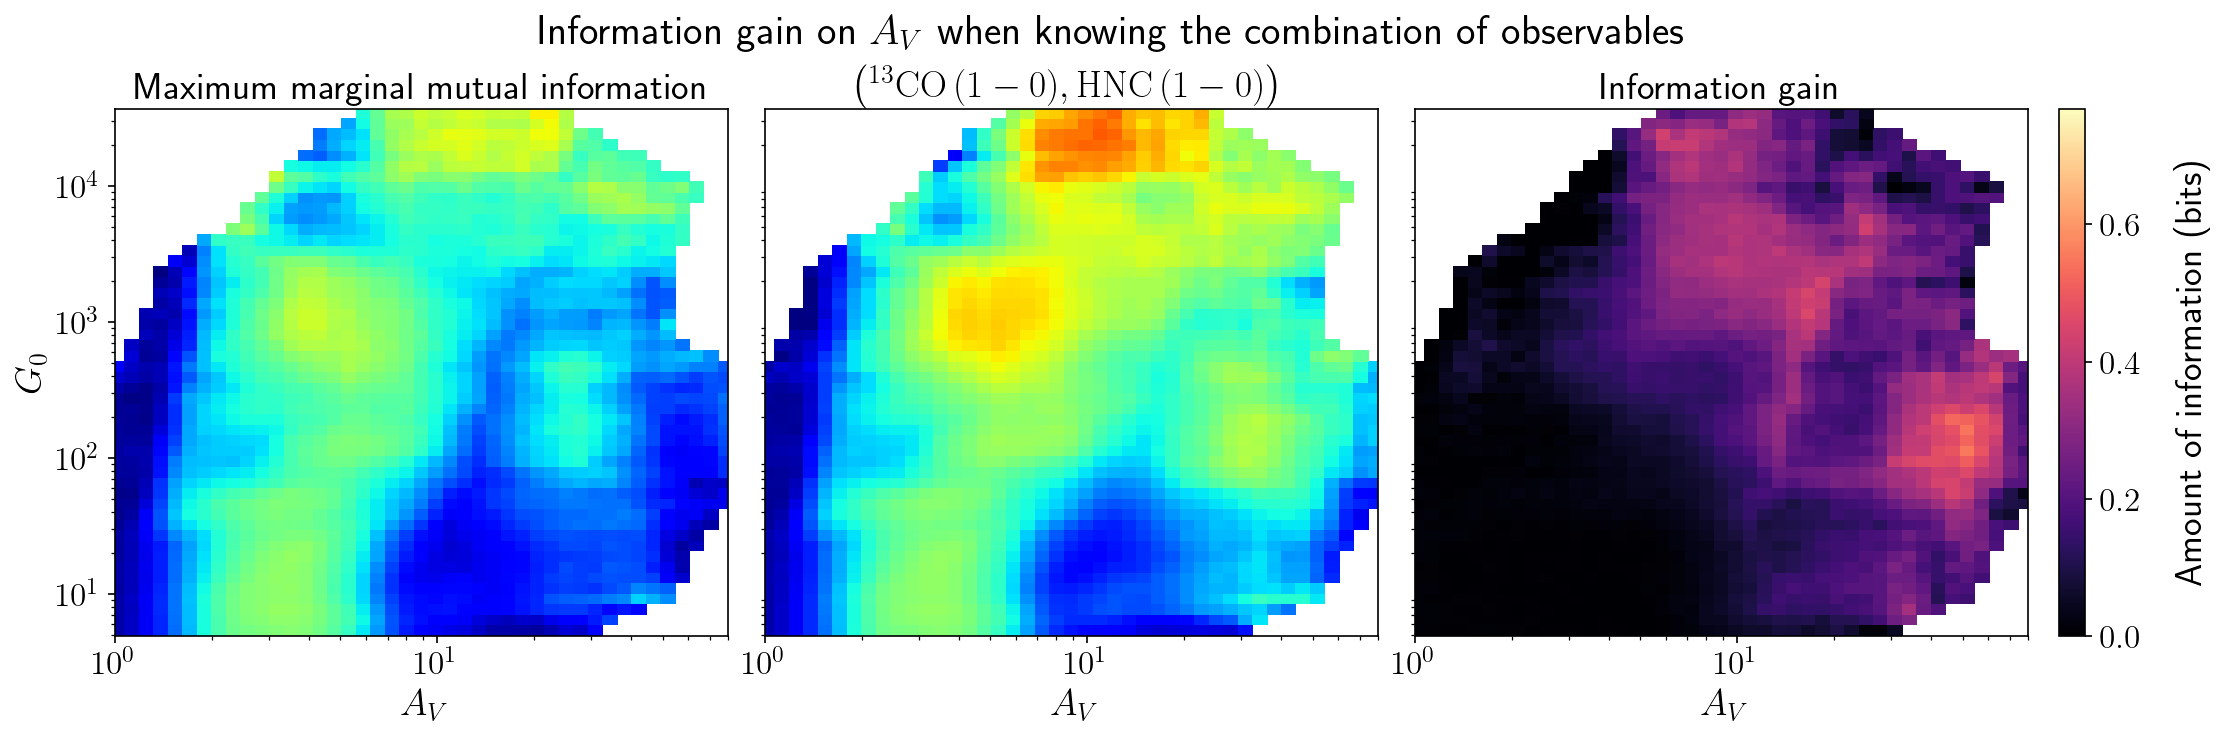
\includegraphics[width=0.95\linewidth]{../mi/av__13co10_hnc10_mi_gain.png}
    \end{figure}
\end{frame}

\begin{frame}{Informativity on $A_V$ of $\left(\mathrm{^{13}CO\,(1-0)},\mathrm{N_2H^+\,(1-0)}\right)$}
    \begin{figure}
        \centering
        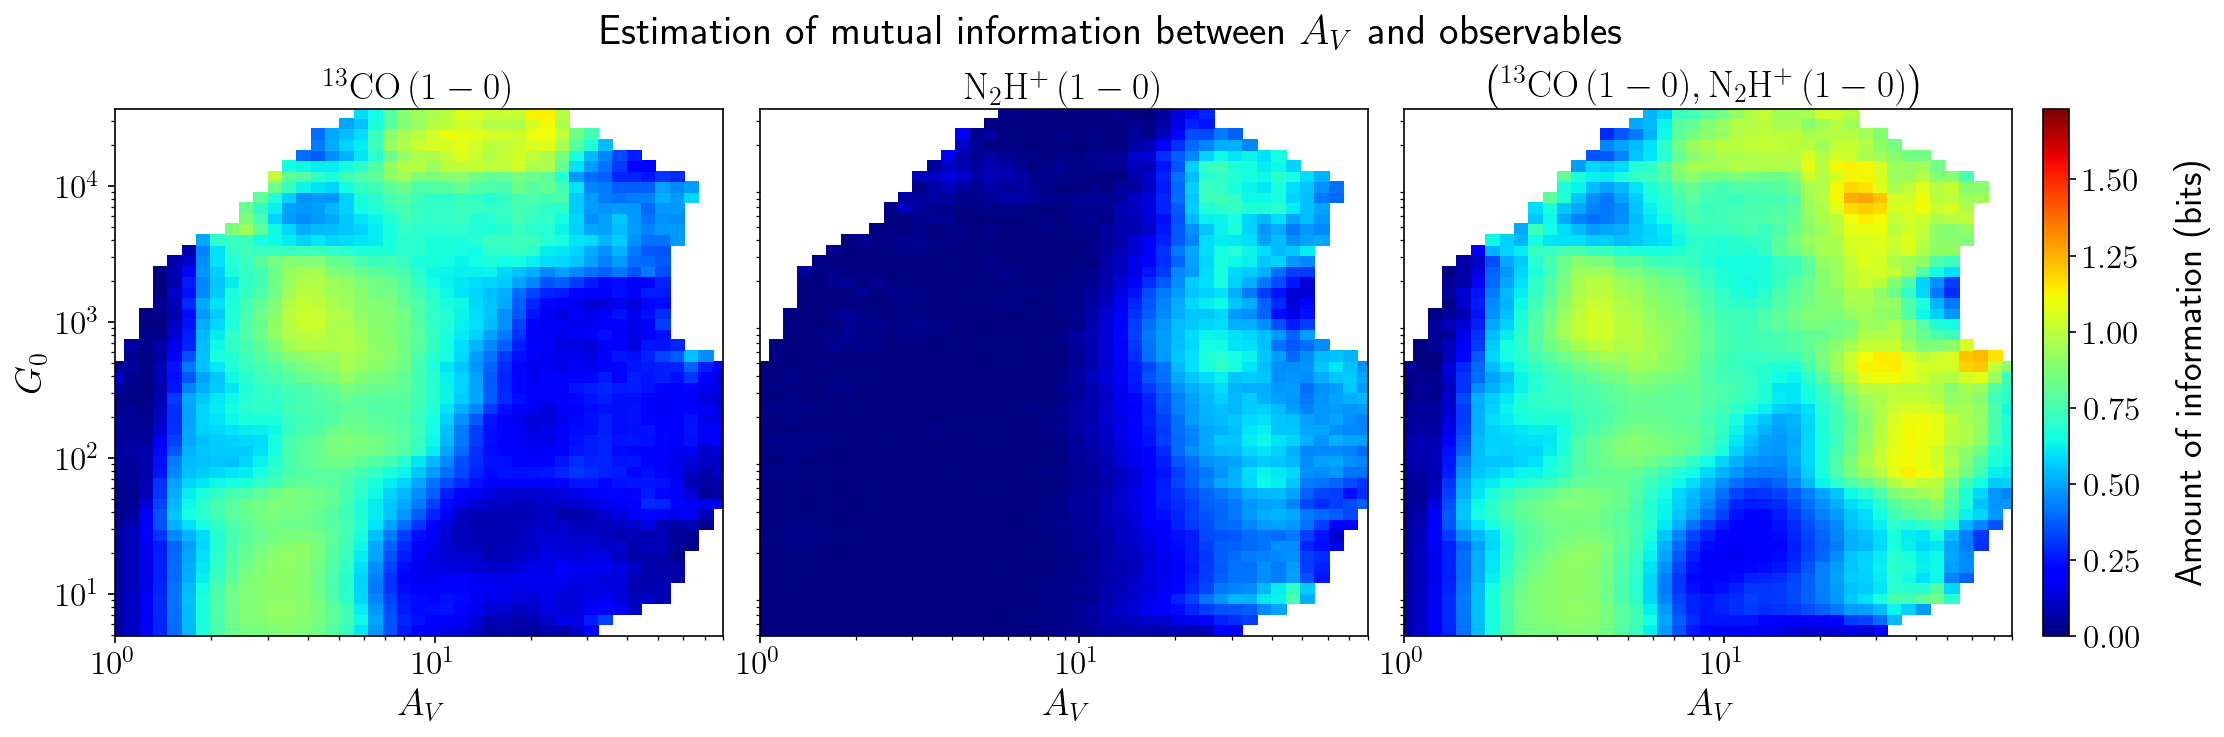
\includegraphics[width=0.95\linewidth]{../mi/av__13co10_n2hp10_mi.png}
        \vfill
        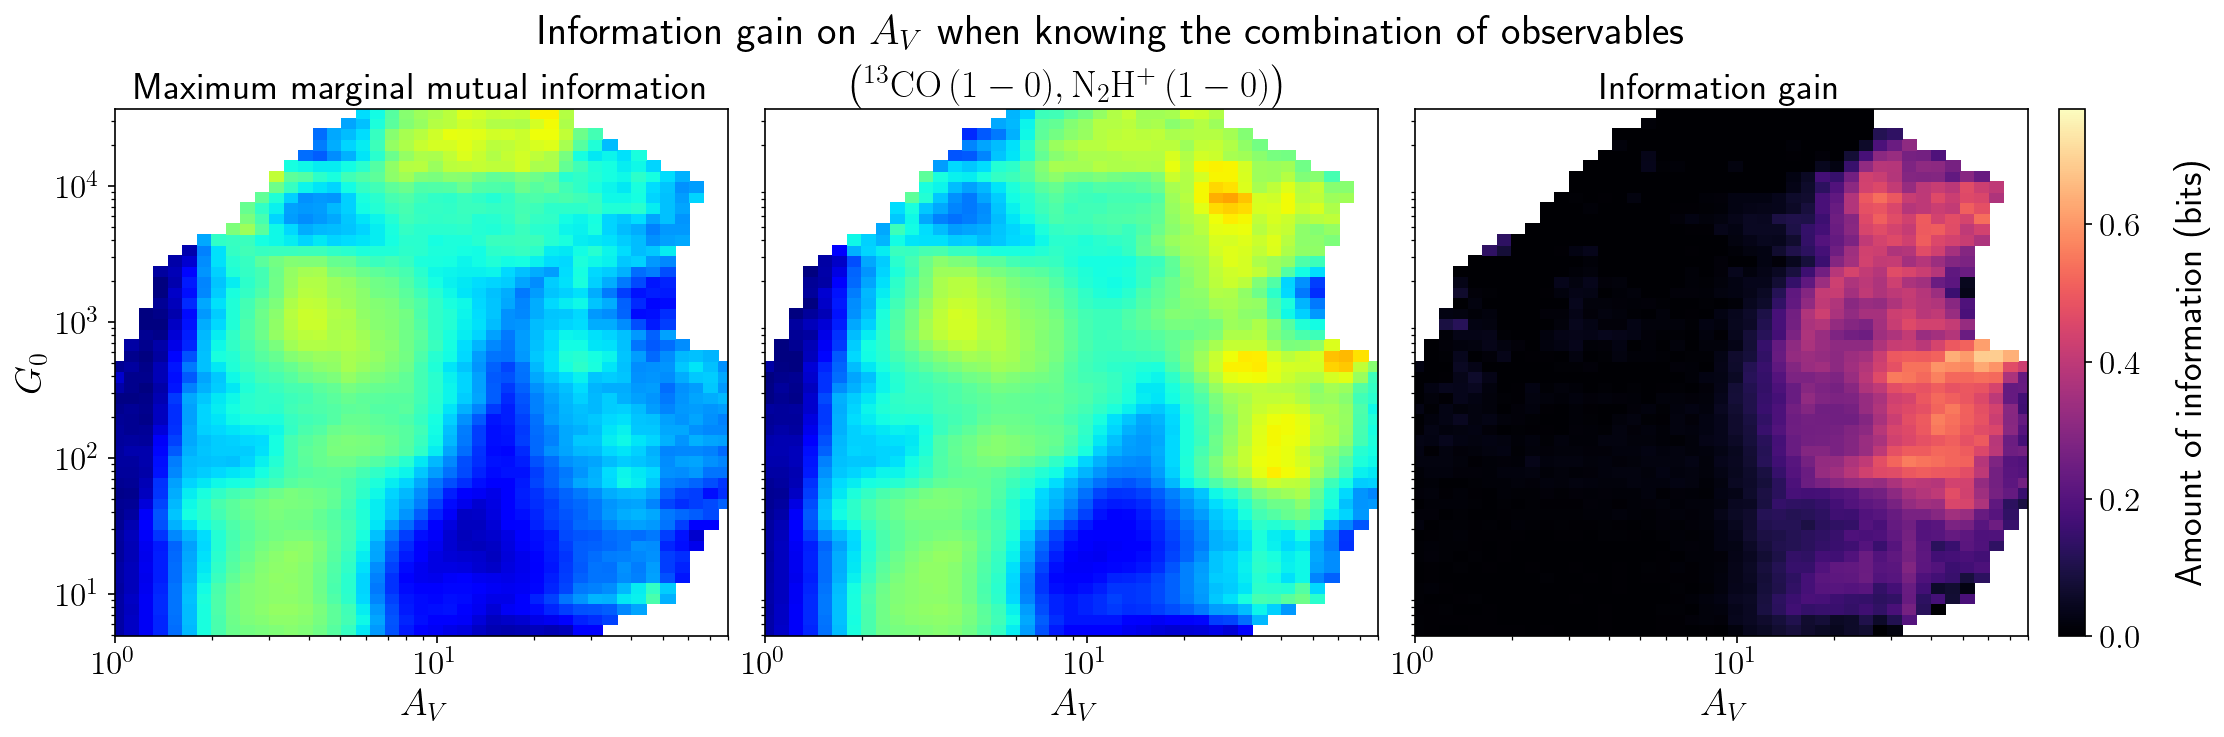
\includegraphics[width=0.95\linewidth]{../mi/av__13co10_n2hp10_mi_gain.png}
    \end{figure}
\end{frame}

\section{Combinations including $\mathrm{^{12}CO\,(1-0)}$ (11 available)}

\begin{frame}{Informativity on $A_V$ of $\left(\mathrm{^{12}CN\,(1-0)},\mathrm{^{12}CO\,(1-0)}\right)$}
    \begin{figure}
        \centering
        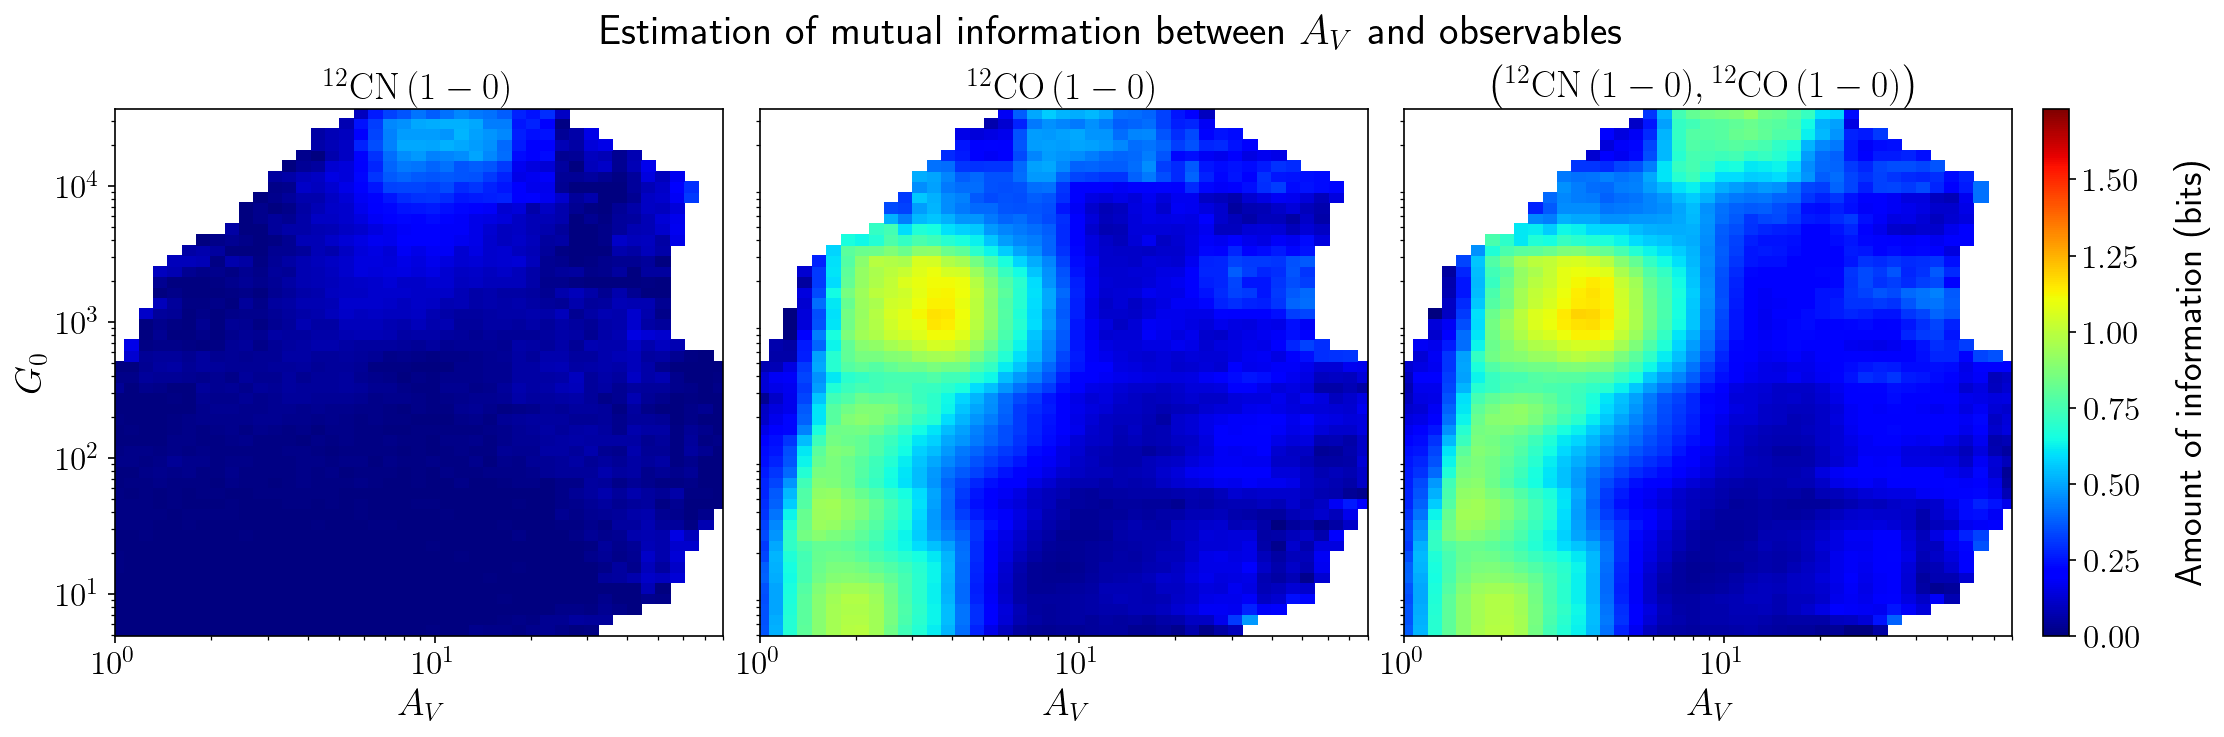
\includegraphics[width=0.95\linewidth]{../mi/av__12cn10_12co10_mi.png}
        \vfill
        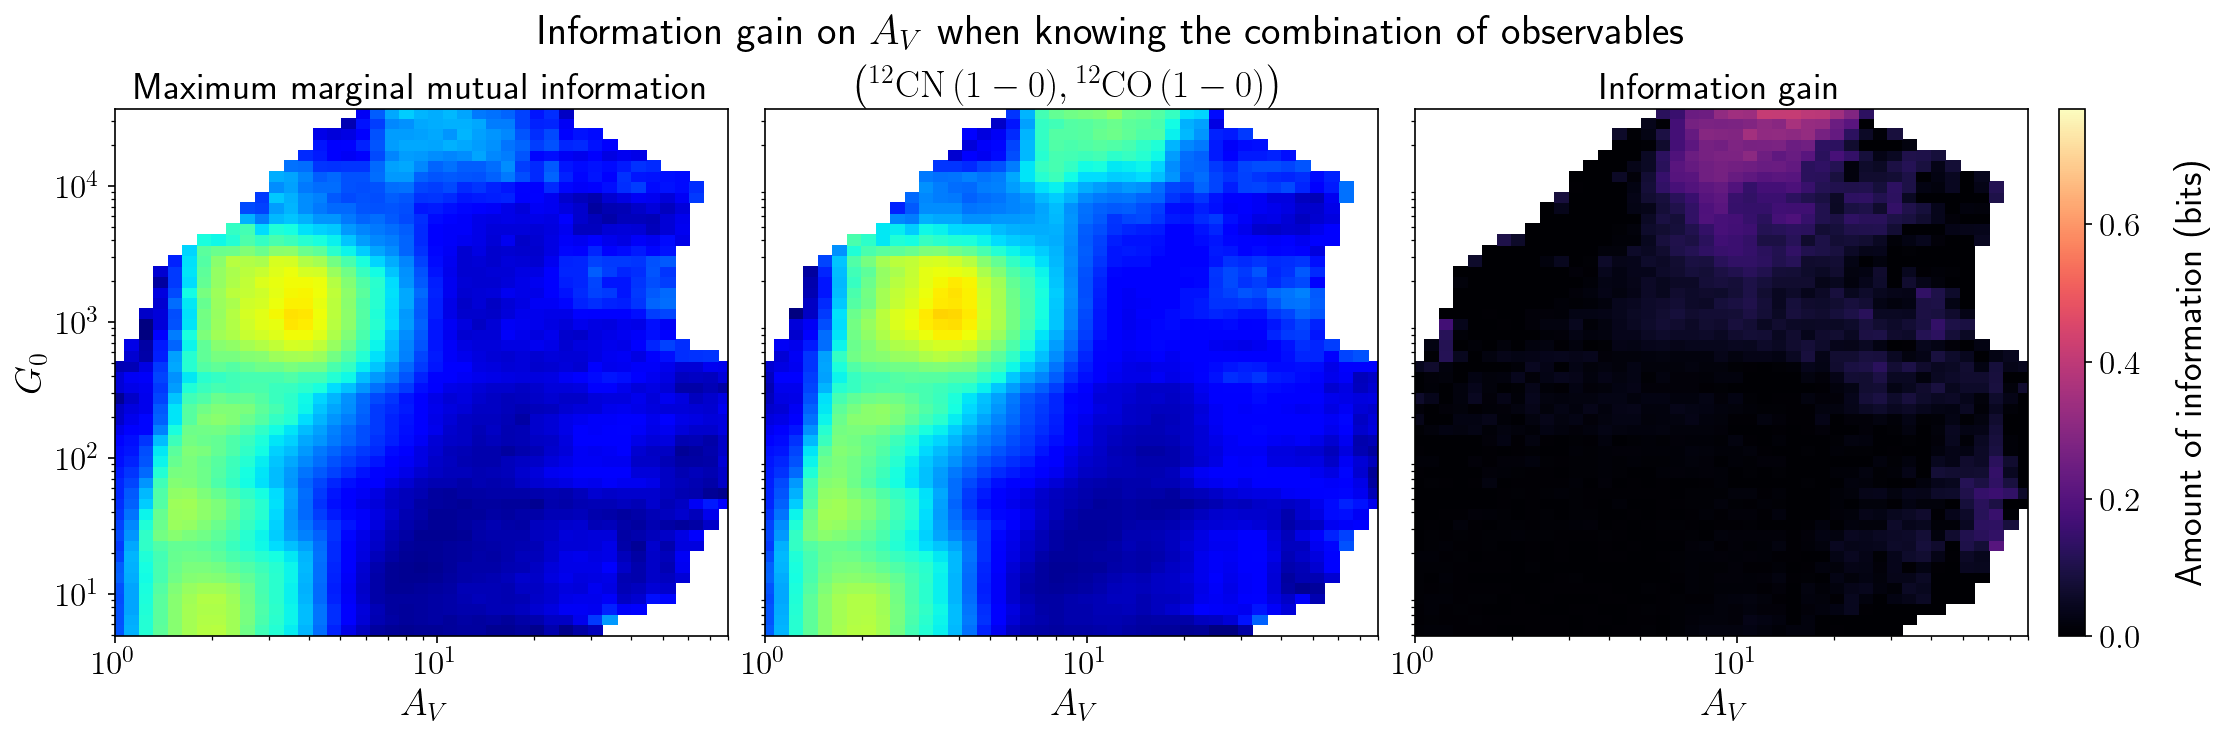
\includegraphics[width=0.95\linewidth]{../mi/av__12cn10_12co10_mi_gain.png}
    \end{figure}
\end{frame}

\begin{frame}{Informativity on $A_V$ of $\left(\mathrm{^{12}CO\,(1-0)},\mathrm{^{12}CS\,(2-1)}\right)$}
    \begin{figure}
        \centering
        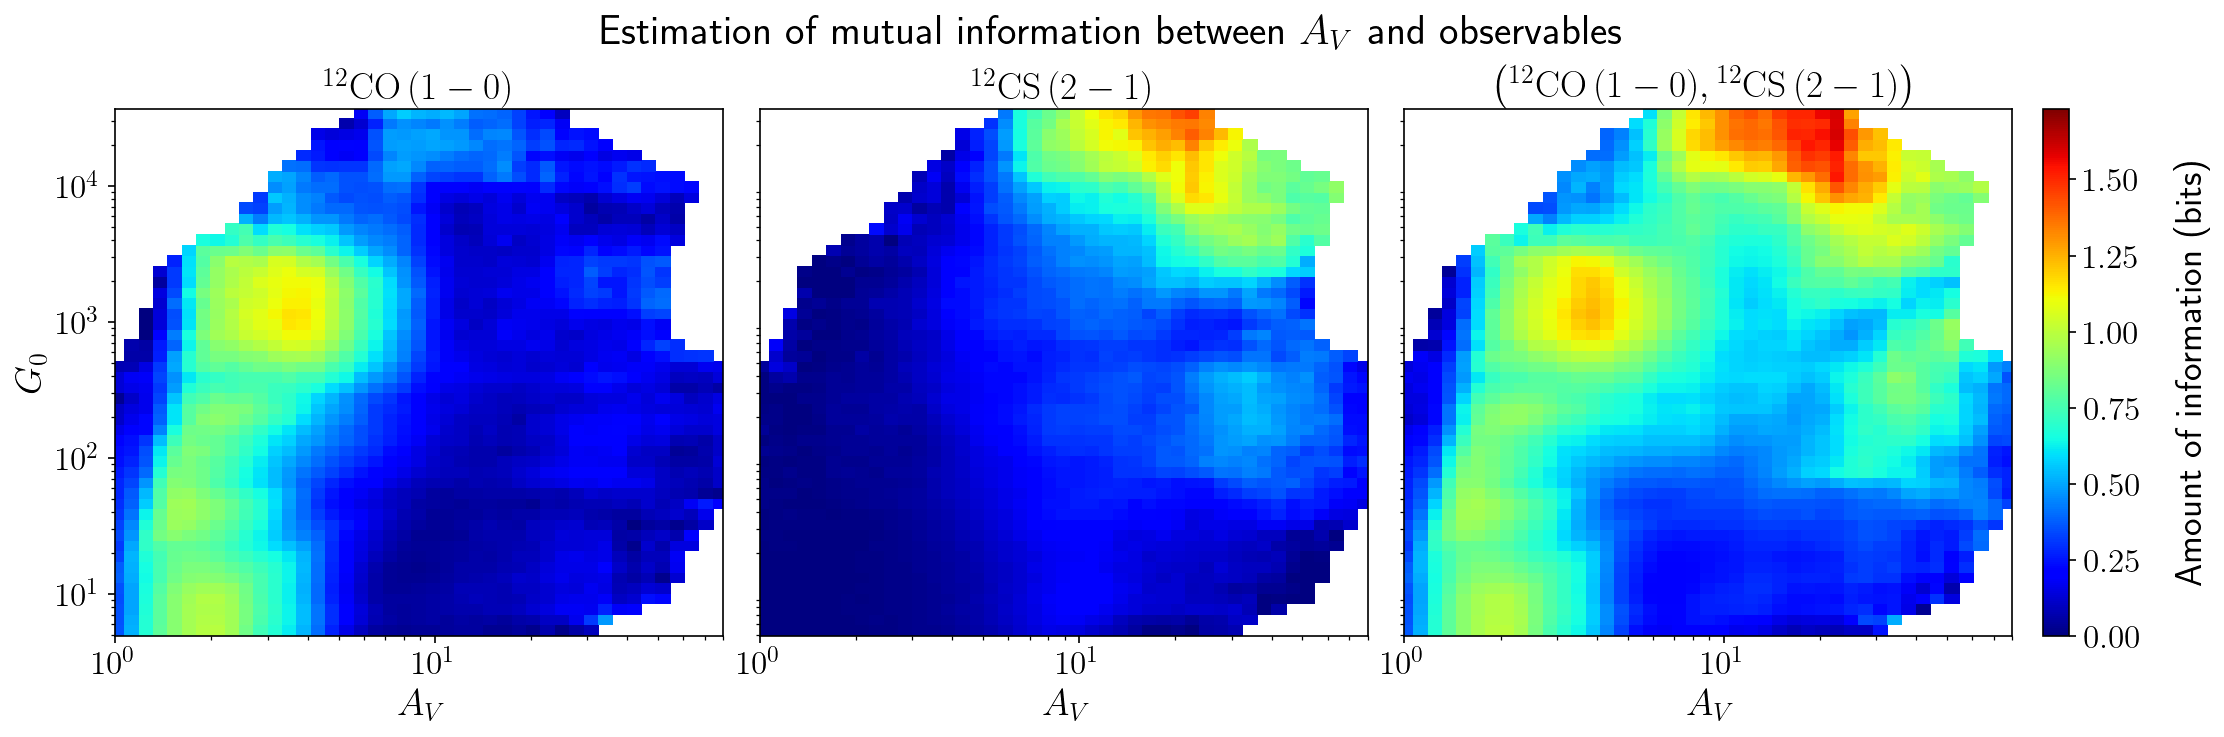
\includegraphics[width=0.95\linewidth]{../mi/av__12co10_12cs21_mi.png}
        \vfill
        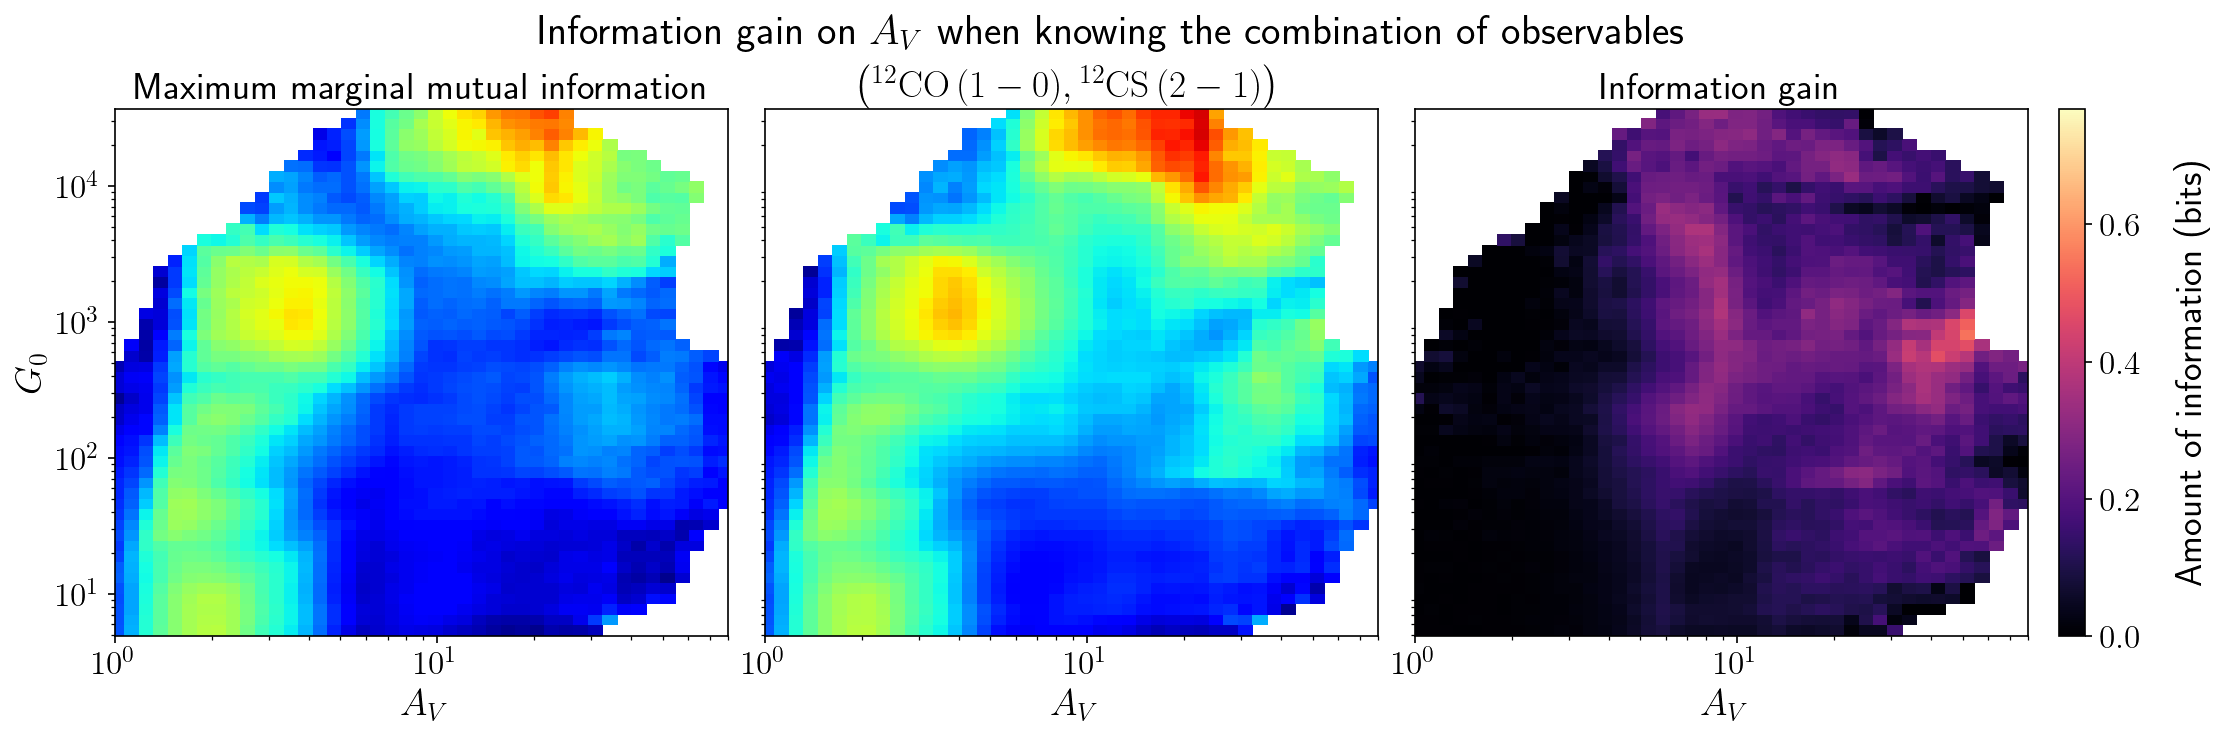
\includegraphics[width=0.95\linewidth]{../mi/av__12co10_12cs21_mi_gain.png}
    \end{figure}
\end{frame}

\begin{frame}{Informativity on $A_V$ of $\left(\mathrm{^{12}CO\,(1-0)},\mathrm{^{13}CO\,(1-0)}\right)$}
    \begin{figure}
        \centering
        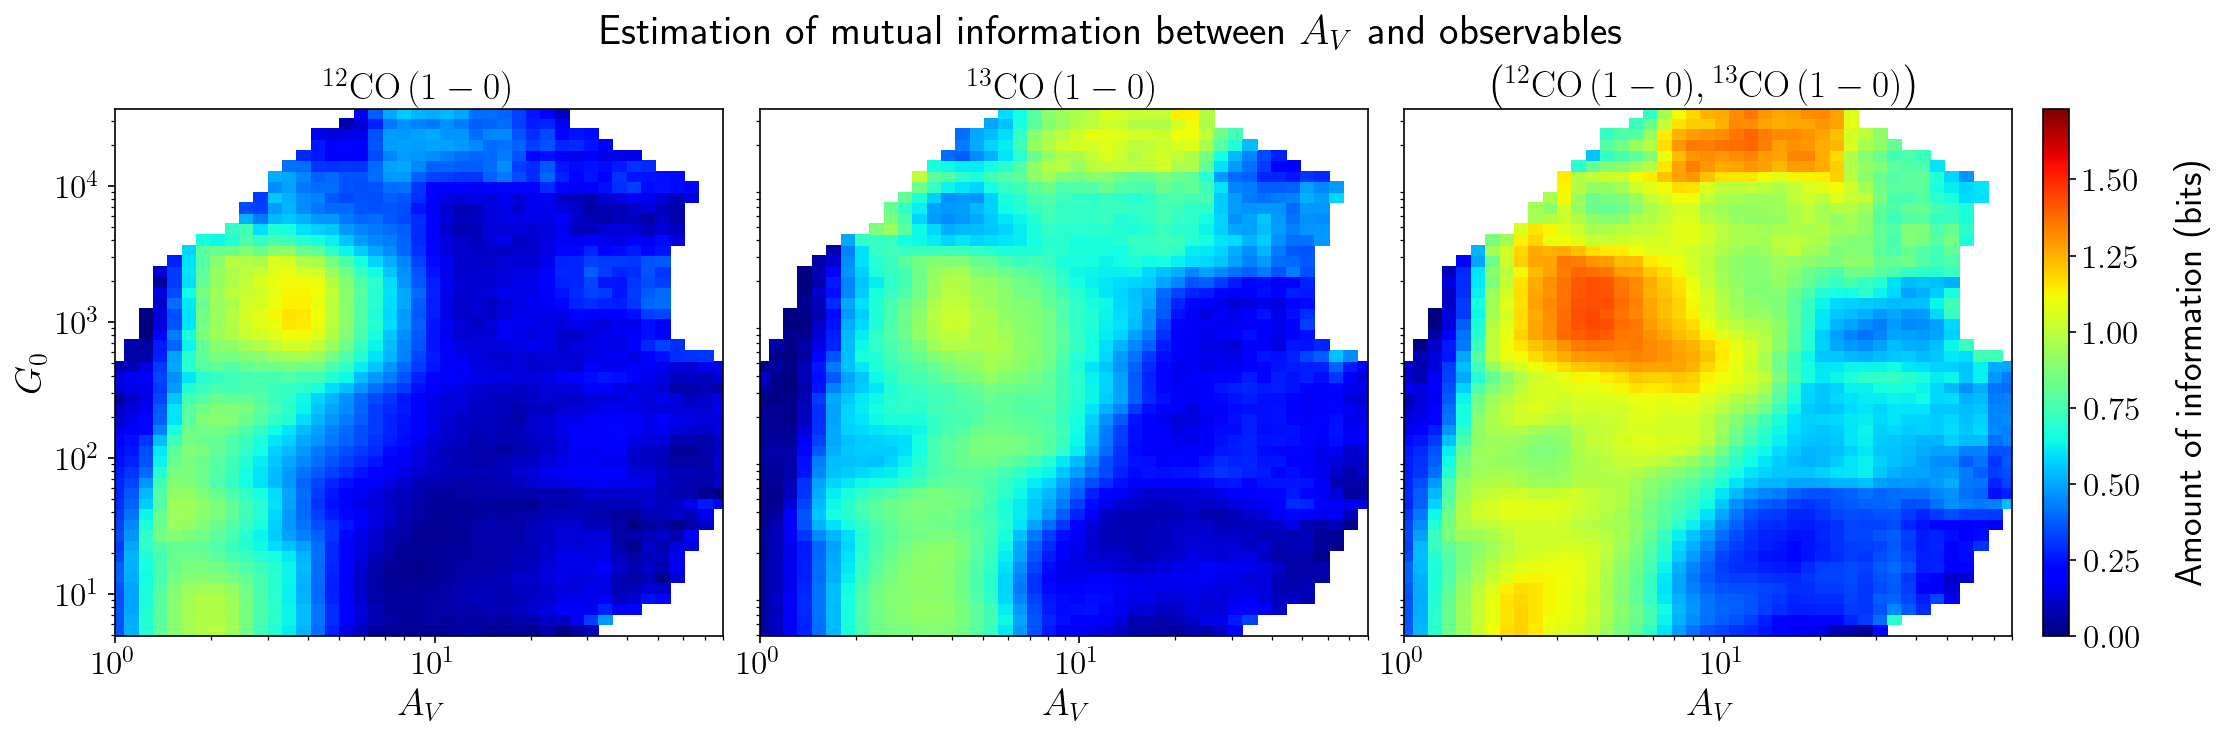
\includegraphics[width=0.95\linewidth]{../mi/av__12co10_13co10_mi.png}
        \vfill
        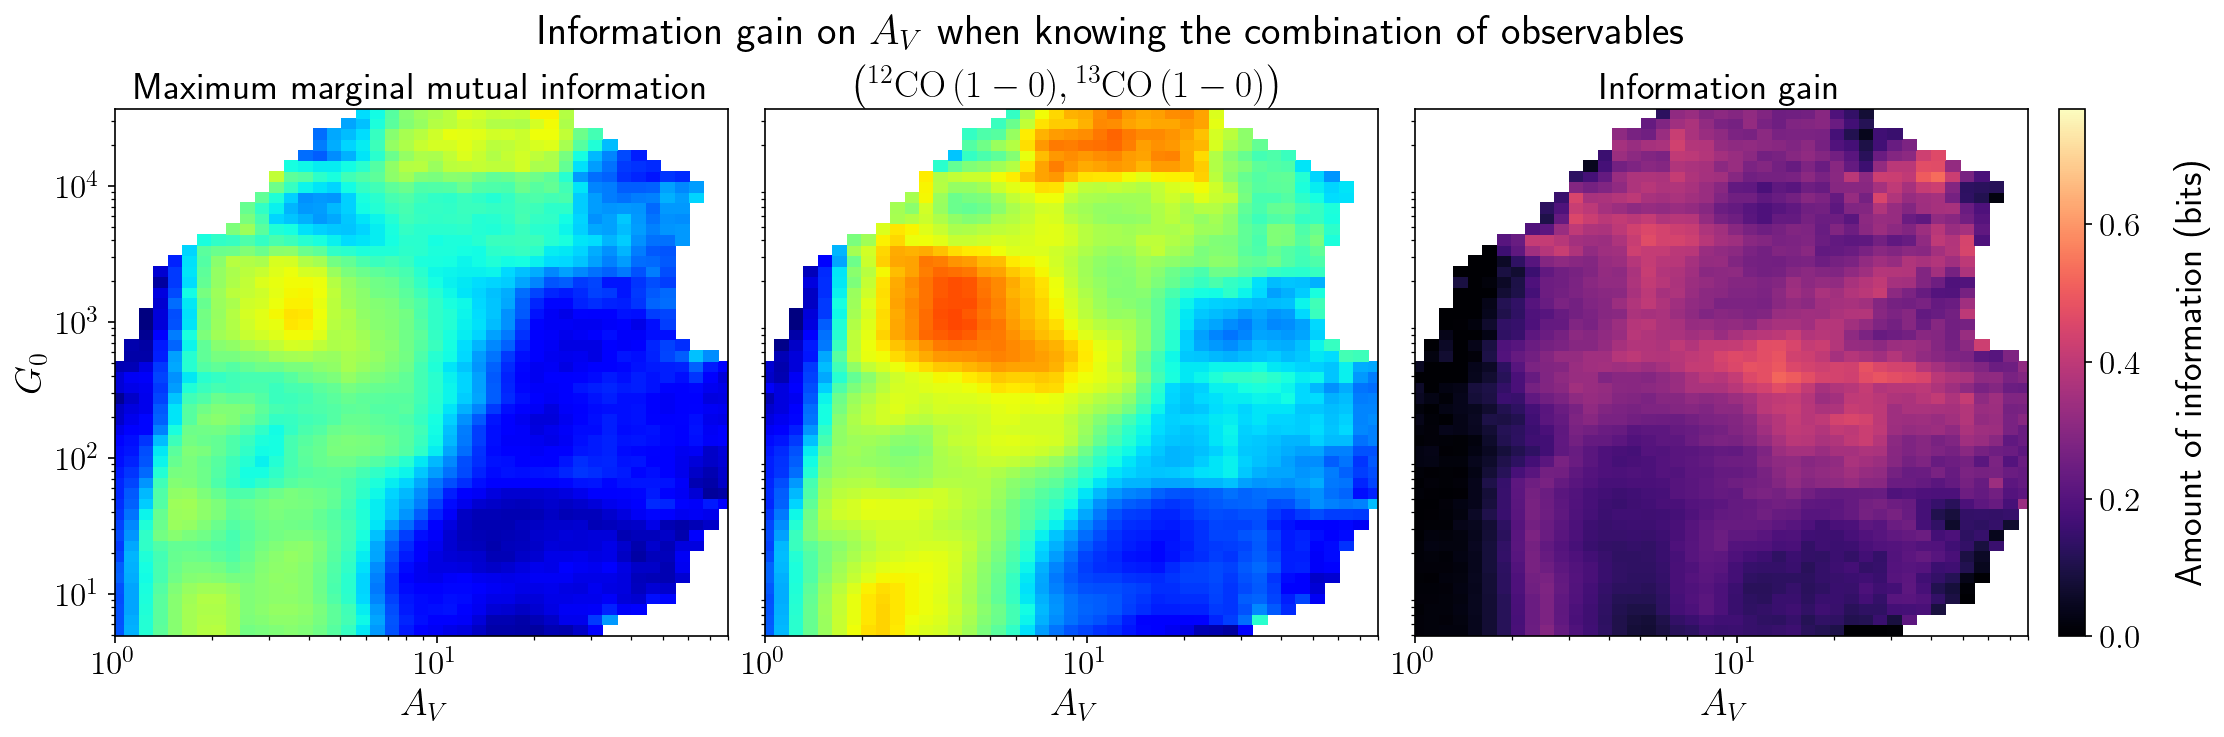
\includegraphics[width=0.95\linewidth]{../mi/av__12co10_13co10_mi_gain.png}
    \end{figure}
\end{frame}

\begin{frame}{Informativity on $A_V$ of $\left(\mathrm{^{12}CO\,(1-0)},\mathrm{^{32}SO\,(2-1)}\right)$}
    \begin{figure}
        \centering
        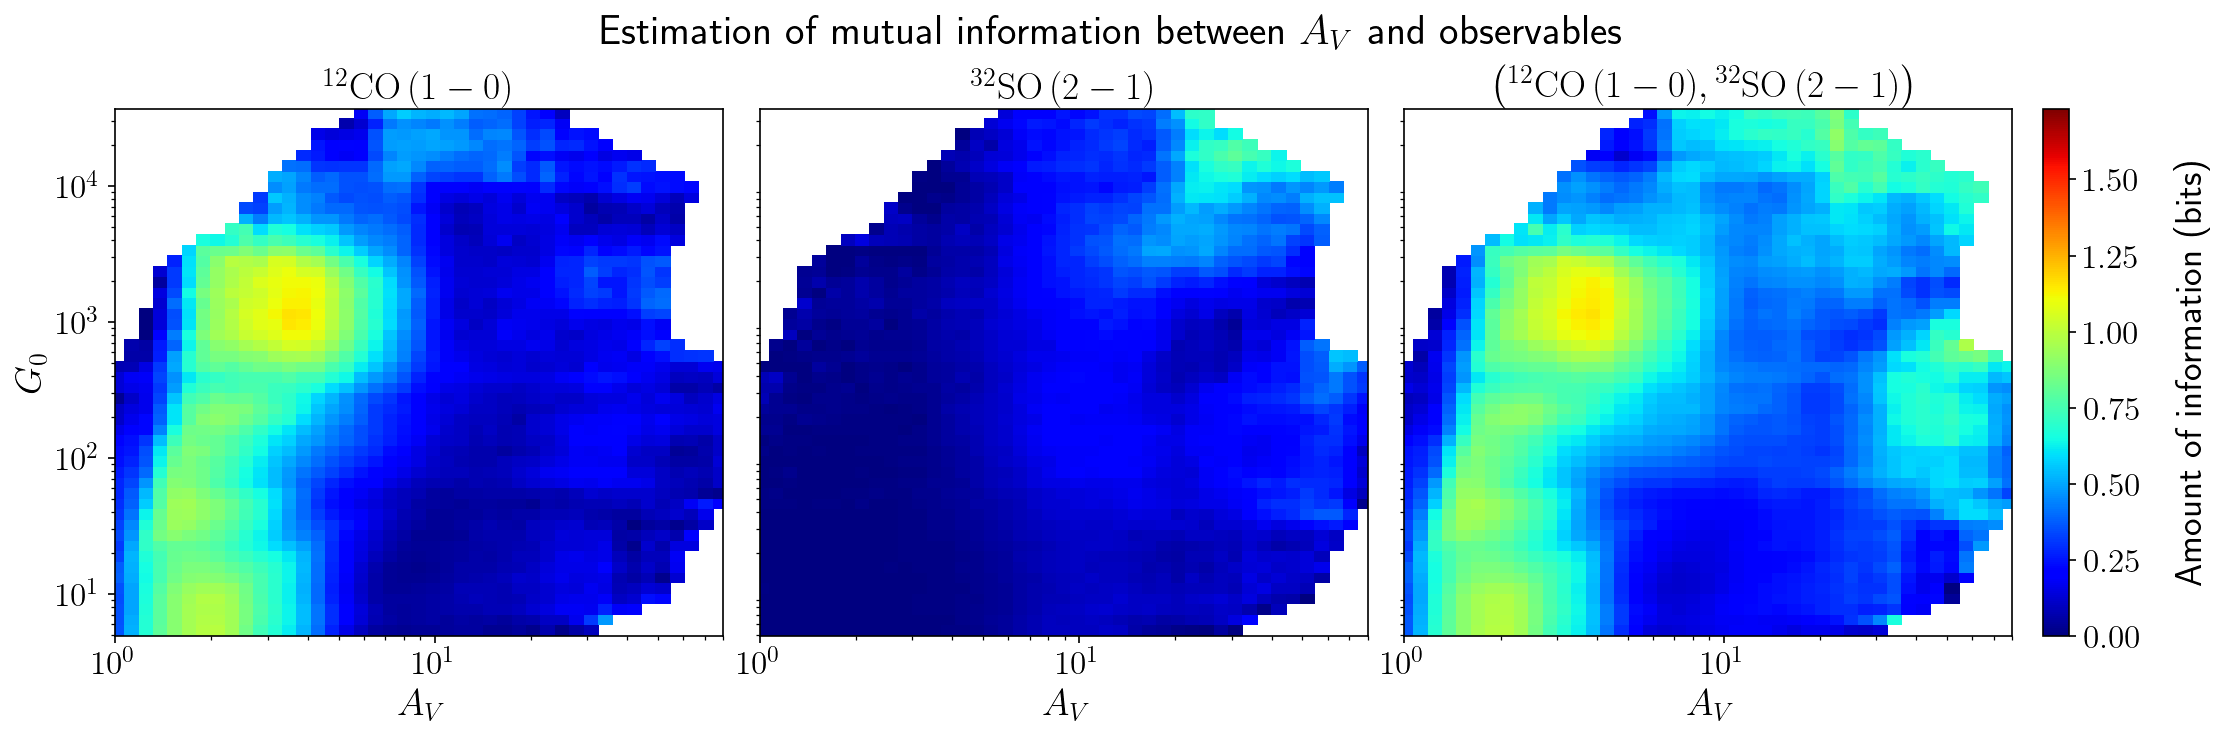
\includegraphics[width=0.95\linewidth]{../mi/av__12co10_32so21_mi.png}
        \vfill
        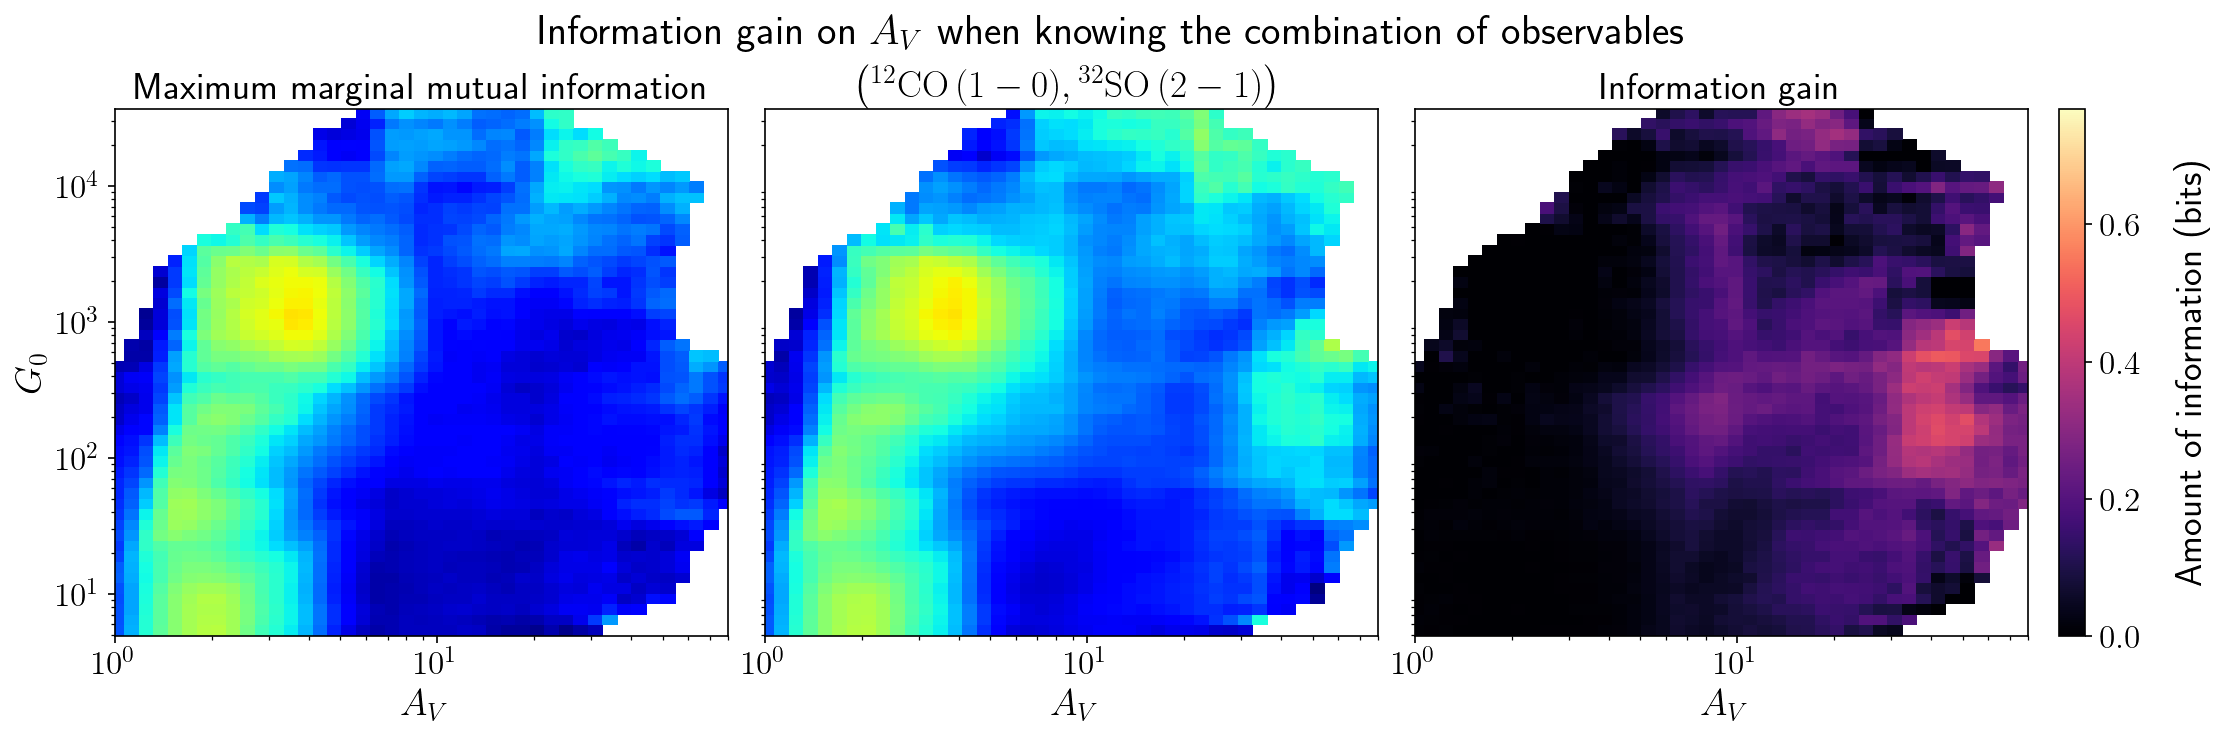
\includegraphics[width=0.95\linewidth]{../mi/av__12co10_32so21_mi_gain.png}
    \end{figure}
\end{frame}

\begin{frame}{Informativity on $A_V$ of $\left(\mathrm{^{12}CO\,(1-0)},\mathrm{C^{18}O\,(1-0)}\right)$}
    \begin{figure}
        \centering
        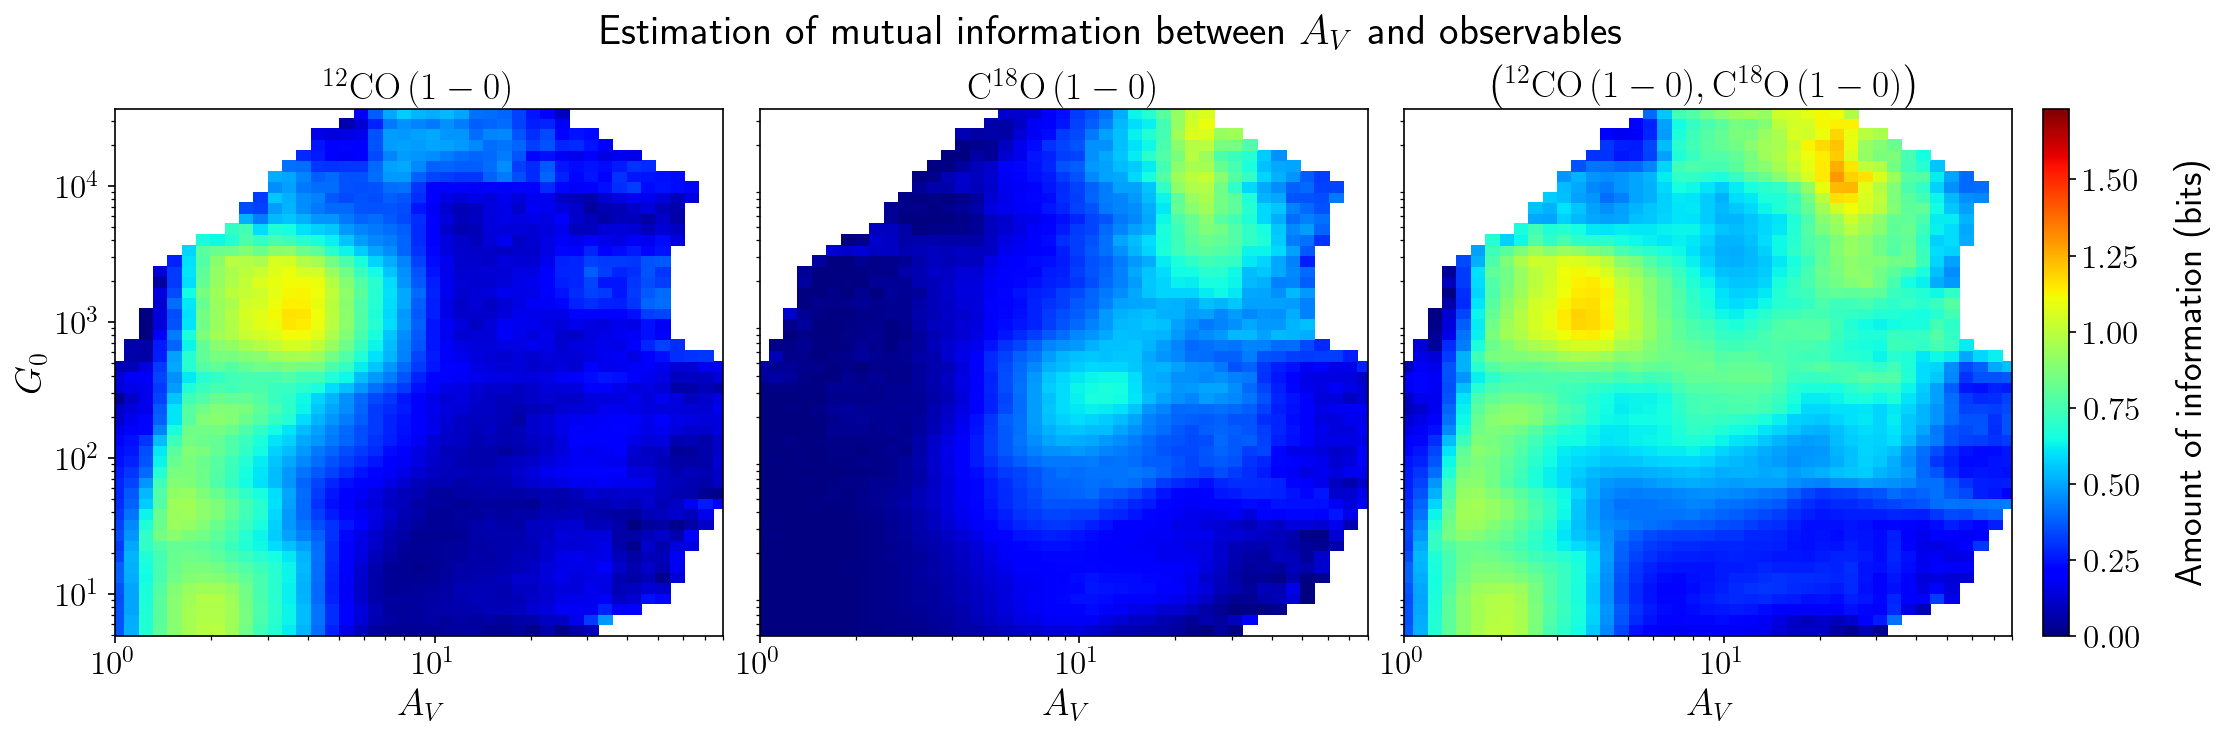
\includegraphics[width=0.95\linewidth]{../mi/av__12co10_c18o10_mi.png}
        \vfill
        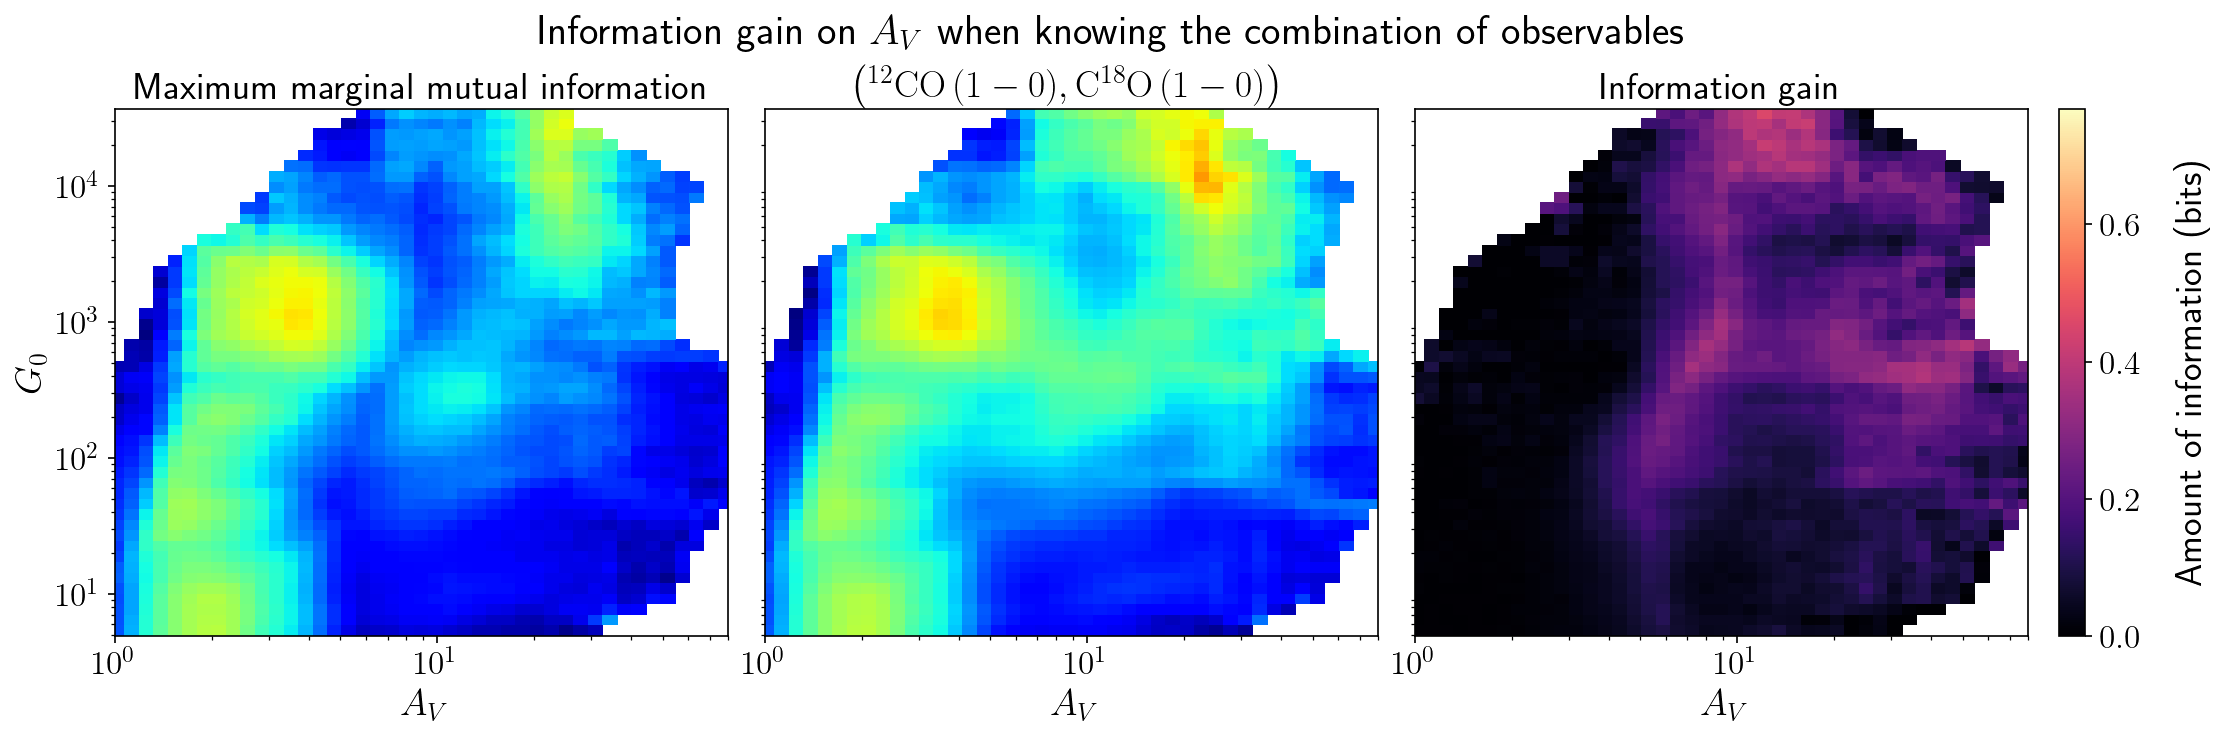
\includegraphics[width=0.95\linewidth]{../mi/av__12co10_c18o10_mi_gain.png}
    \end{figure}
\end{frame}

\begin{frame}{Informativity on $A_V$ of $\left(\mathrm{^{12}CO\,(1-0)},\mathrm{CCH\,(1-0)}\right)$}
    \begin{figure}
        \centering
        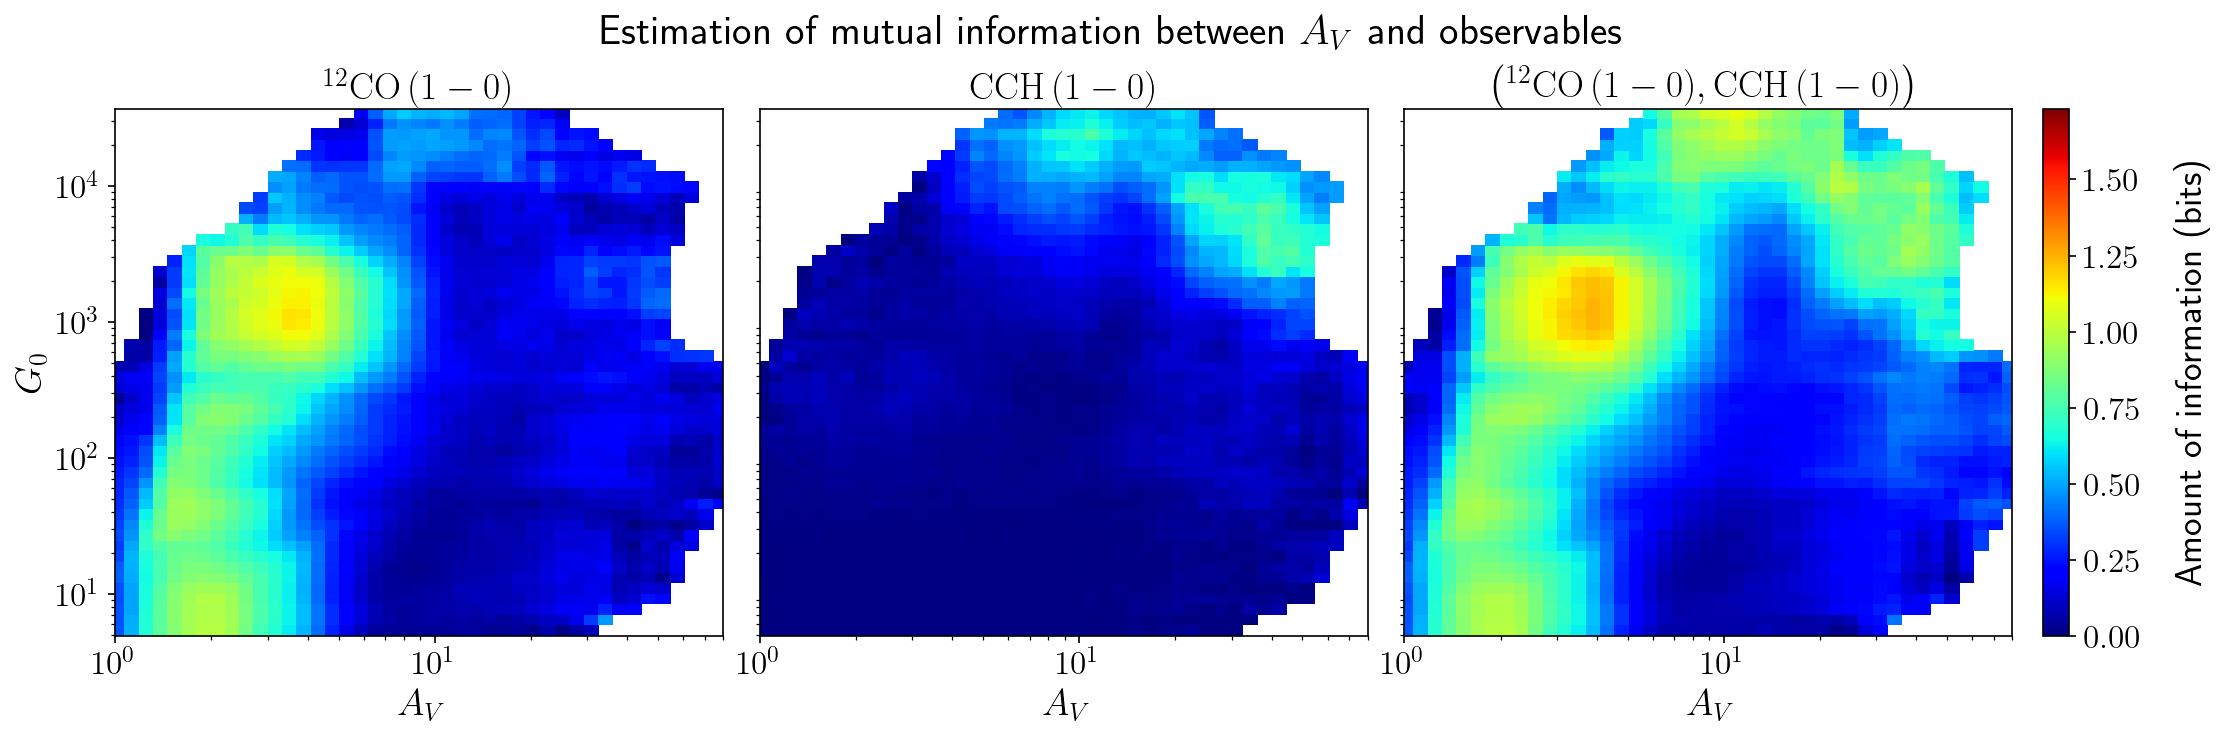
\includegraphics[width=0.95\linewidth]{../mi/av__12co10_cch10_mi.png}
        \vfill
        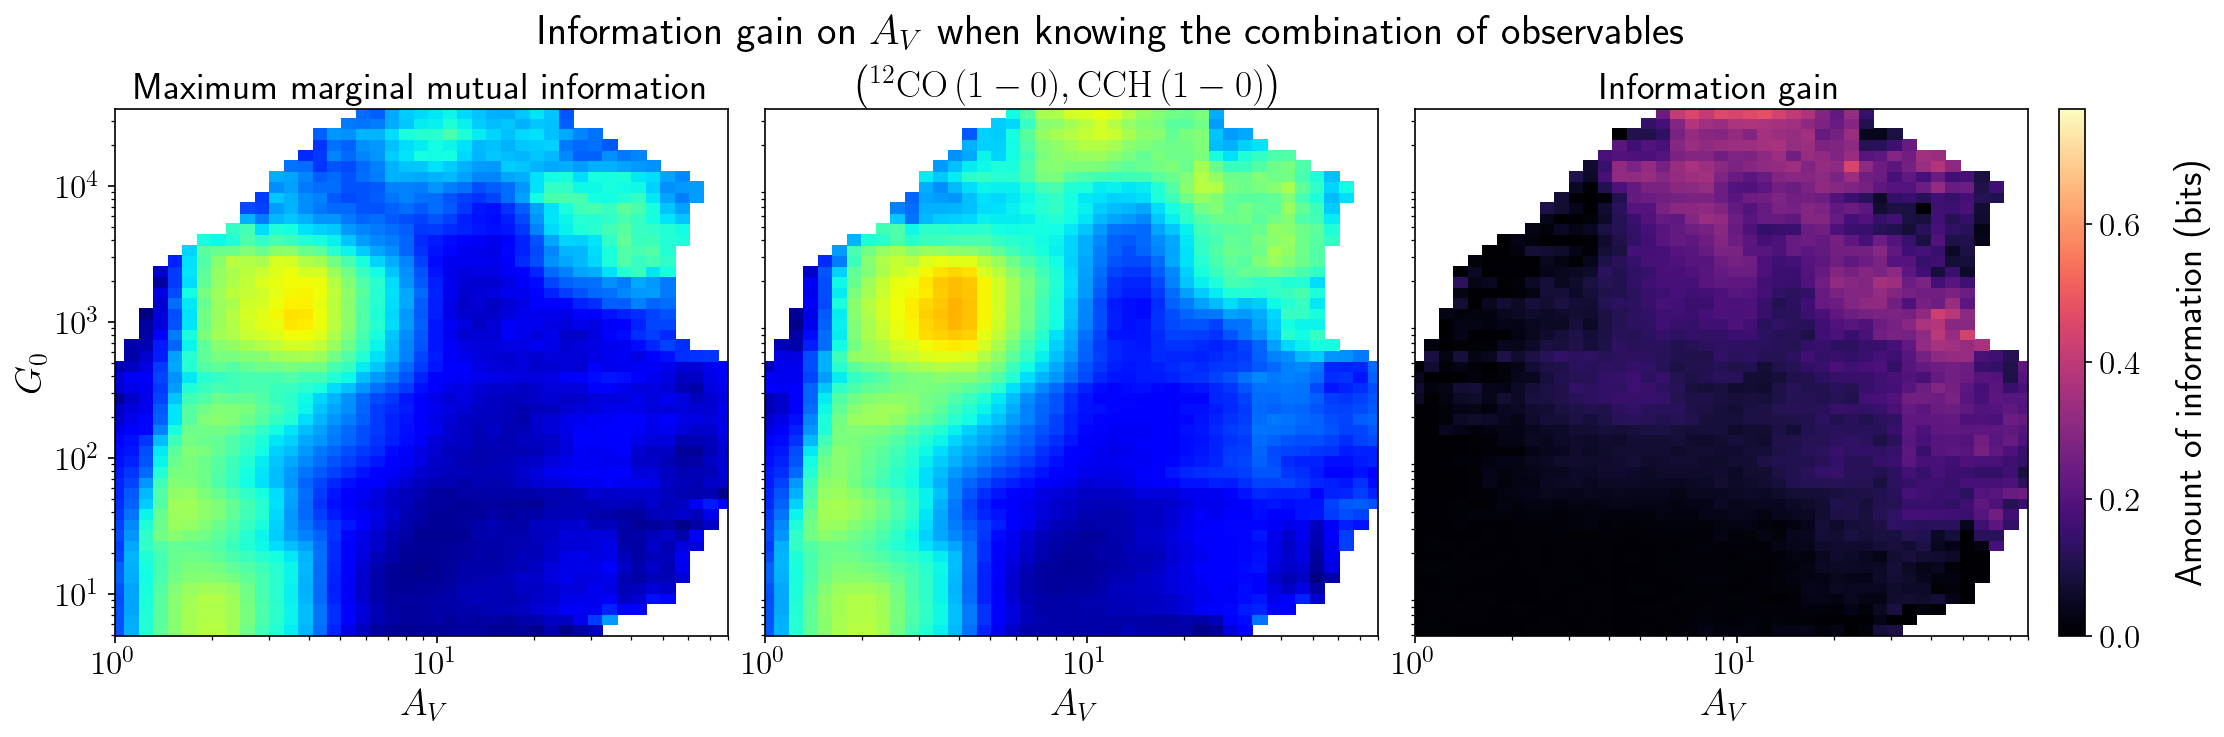
\includegraphics[width=0.95\linewidth]{../mi/av__12co10_cch10_mi_gain.png}
    \end{figure}
\end{frame}

\begin{frame}{Informativity on $A_V$ of $\left(\mathrm{^{12}CO\,(1-0)},\mathrm{H_2CO}\right)$}
    \begin{figure}
        \centering
        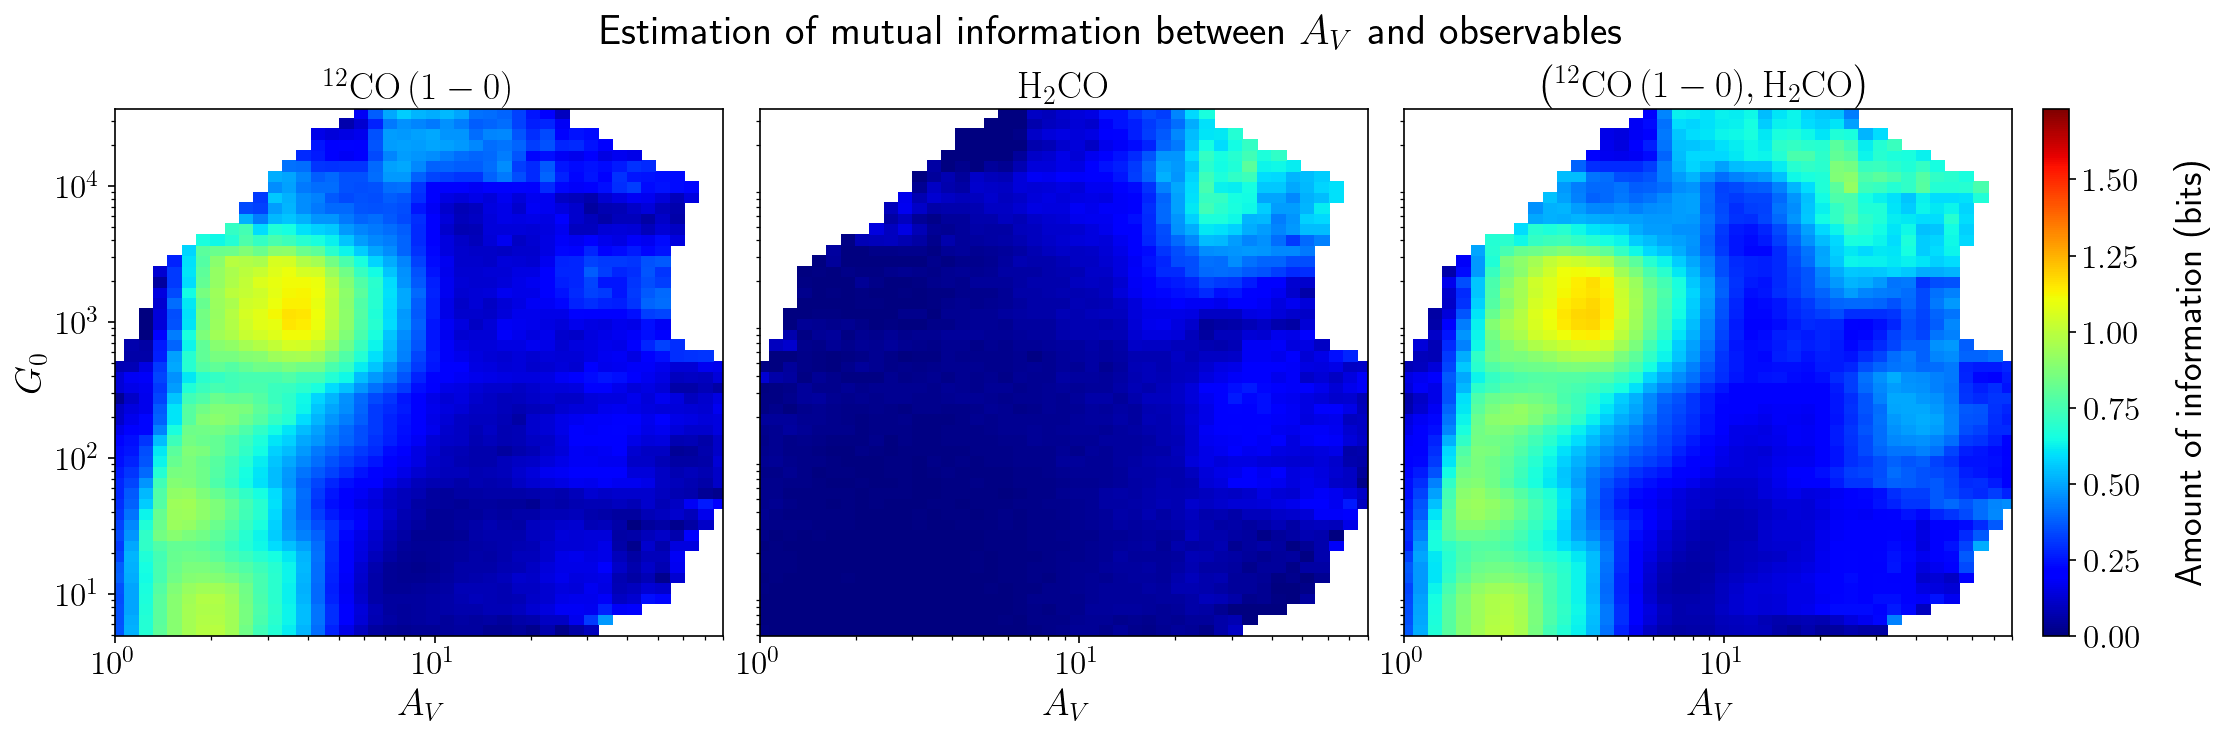
\includegraphics[width=0.95\linewidth]{../mi/av__12co10_h2co_mi.png}
        \vfill
        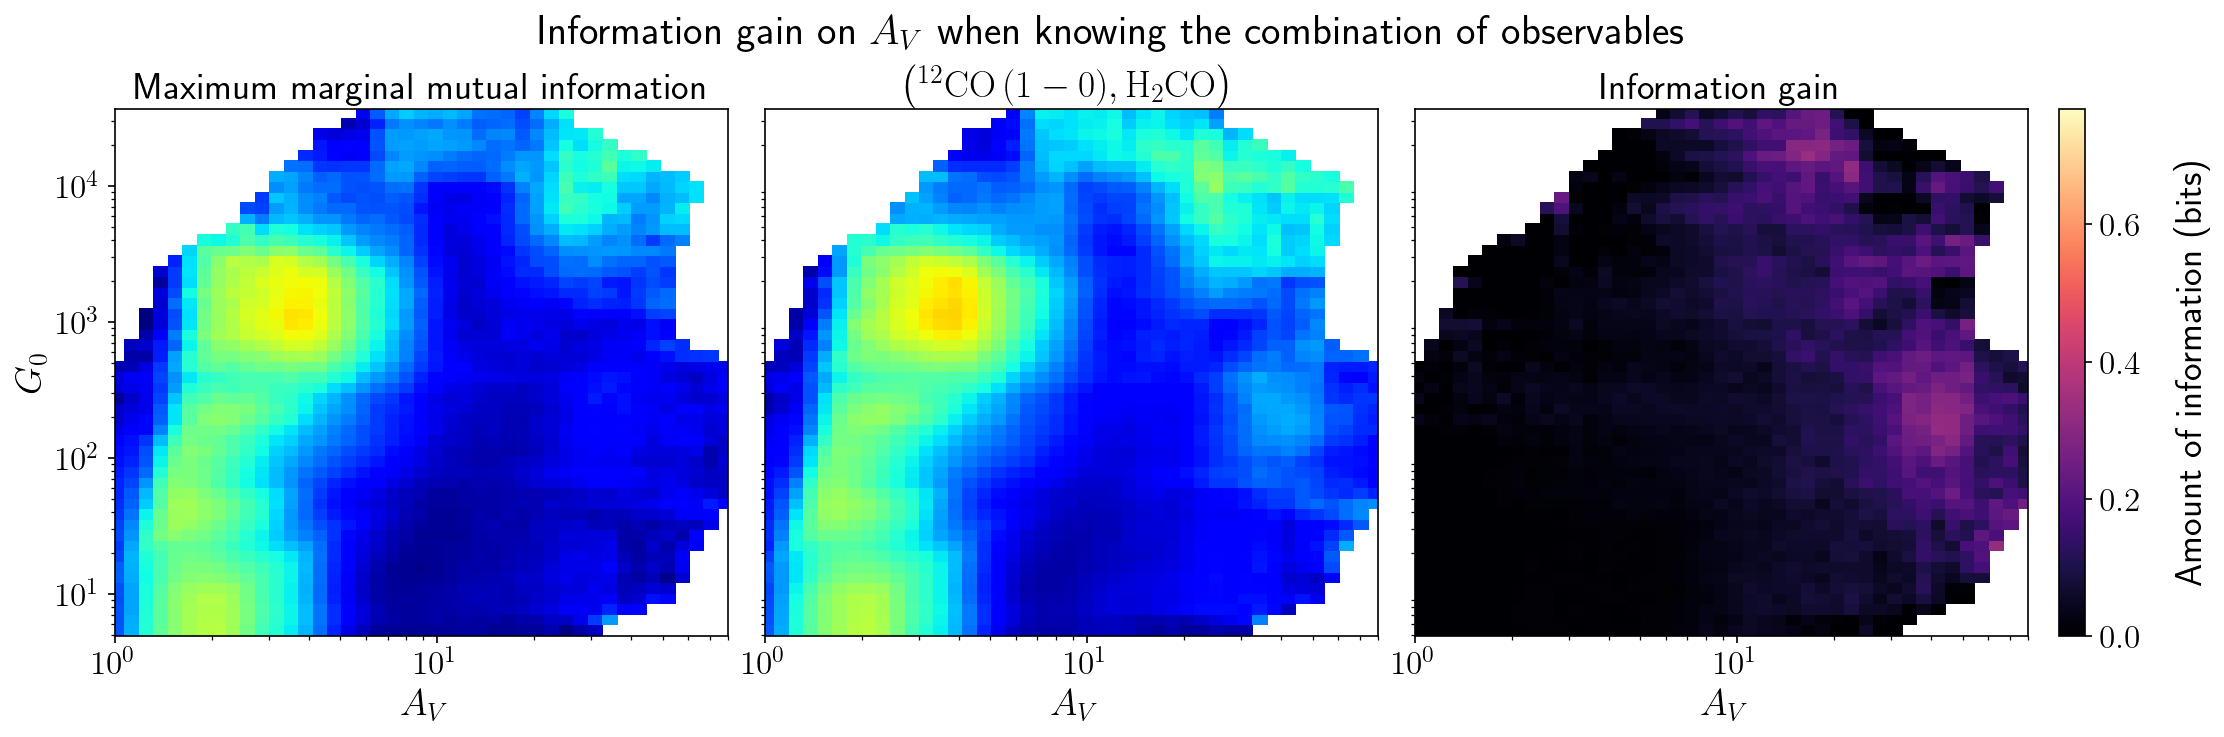
\includegraphics[width=0.95\linewidth]{../mi/av__12co10_h2co_mi_gain.png}
    \end{figure}
\end{frame}

\begin{frame}{Informativity on $A_V$ of $\left(\mathrm{^{12}CO\,(1-0)},\mathrm{HCN\,(1-0)}\right)$}
    \begin{figure}
        \centering
        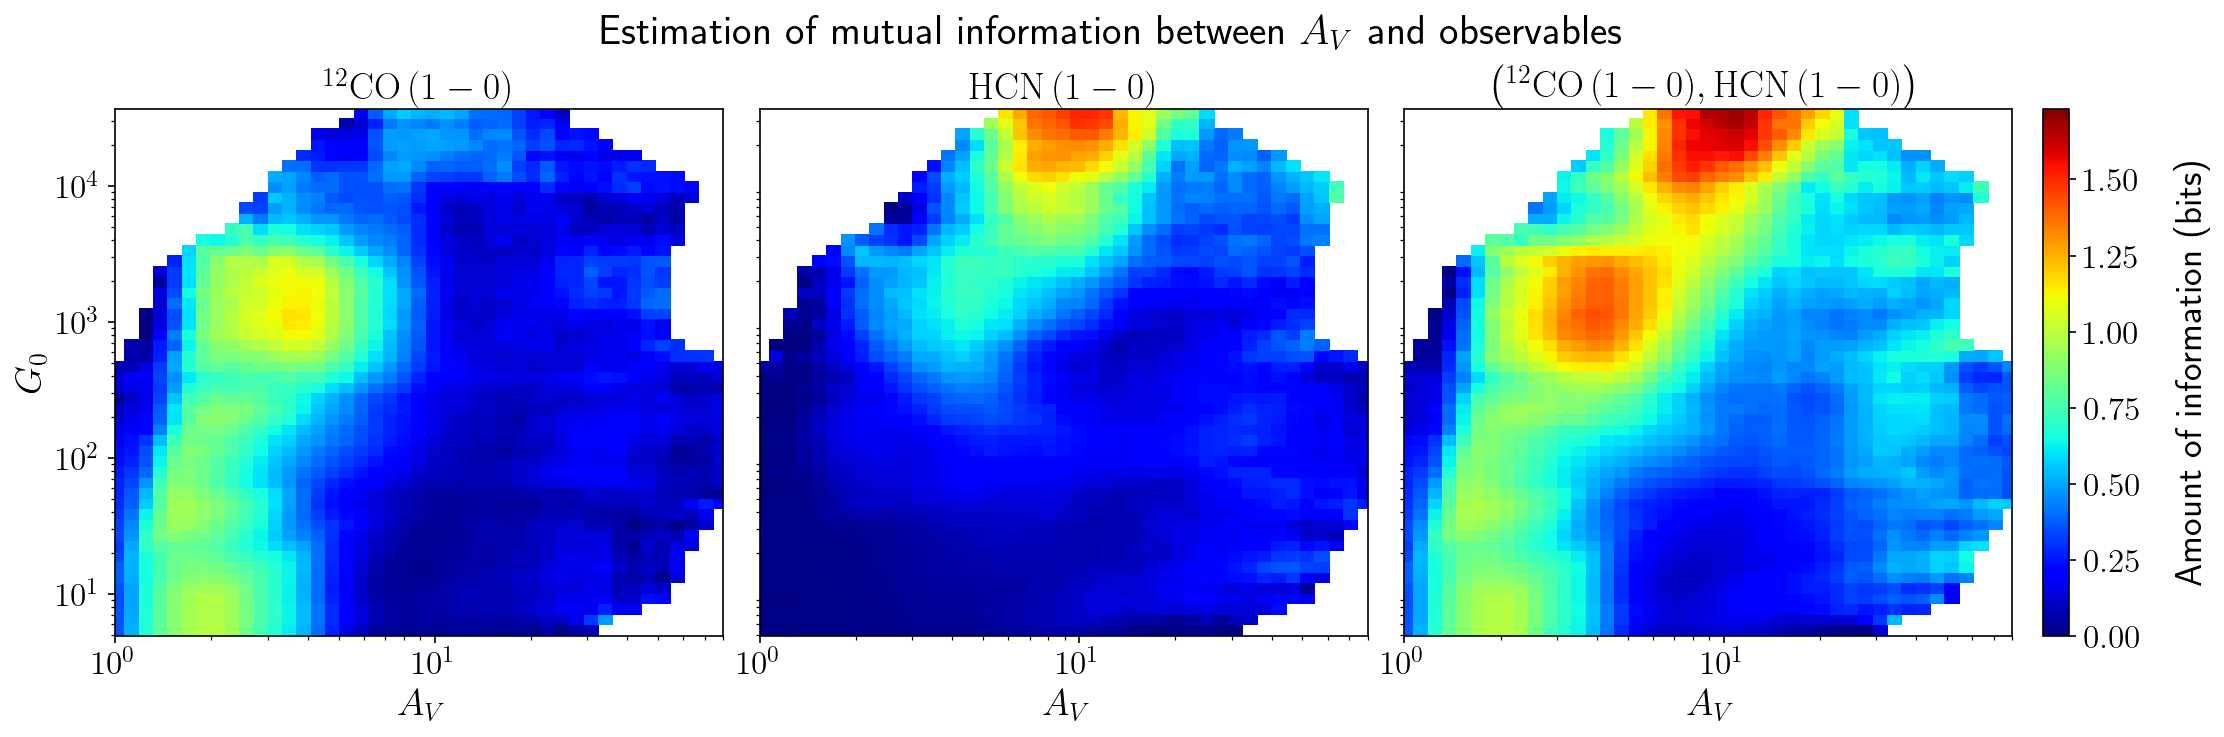
\includegraphics[width=0.95\linewidth]{../mi/av__12co10_hcn10_mi.png}
        \vfill
        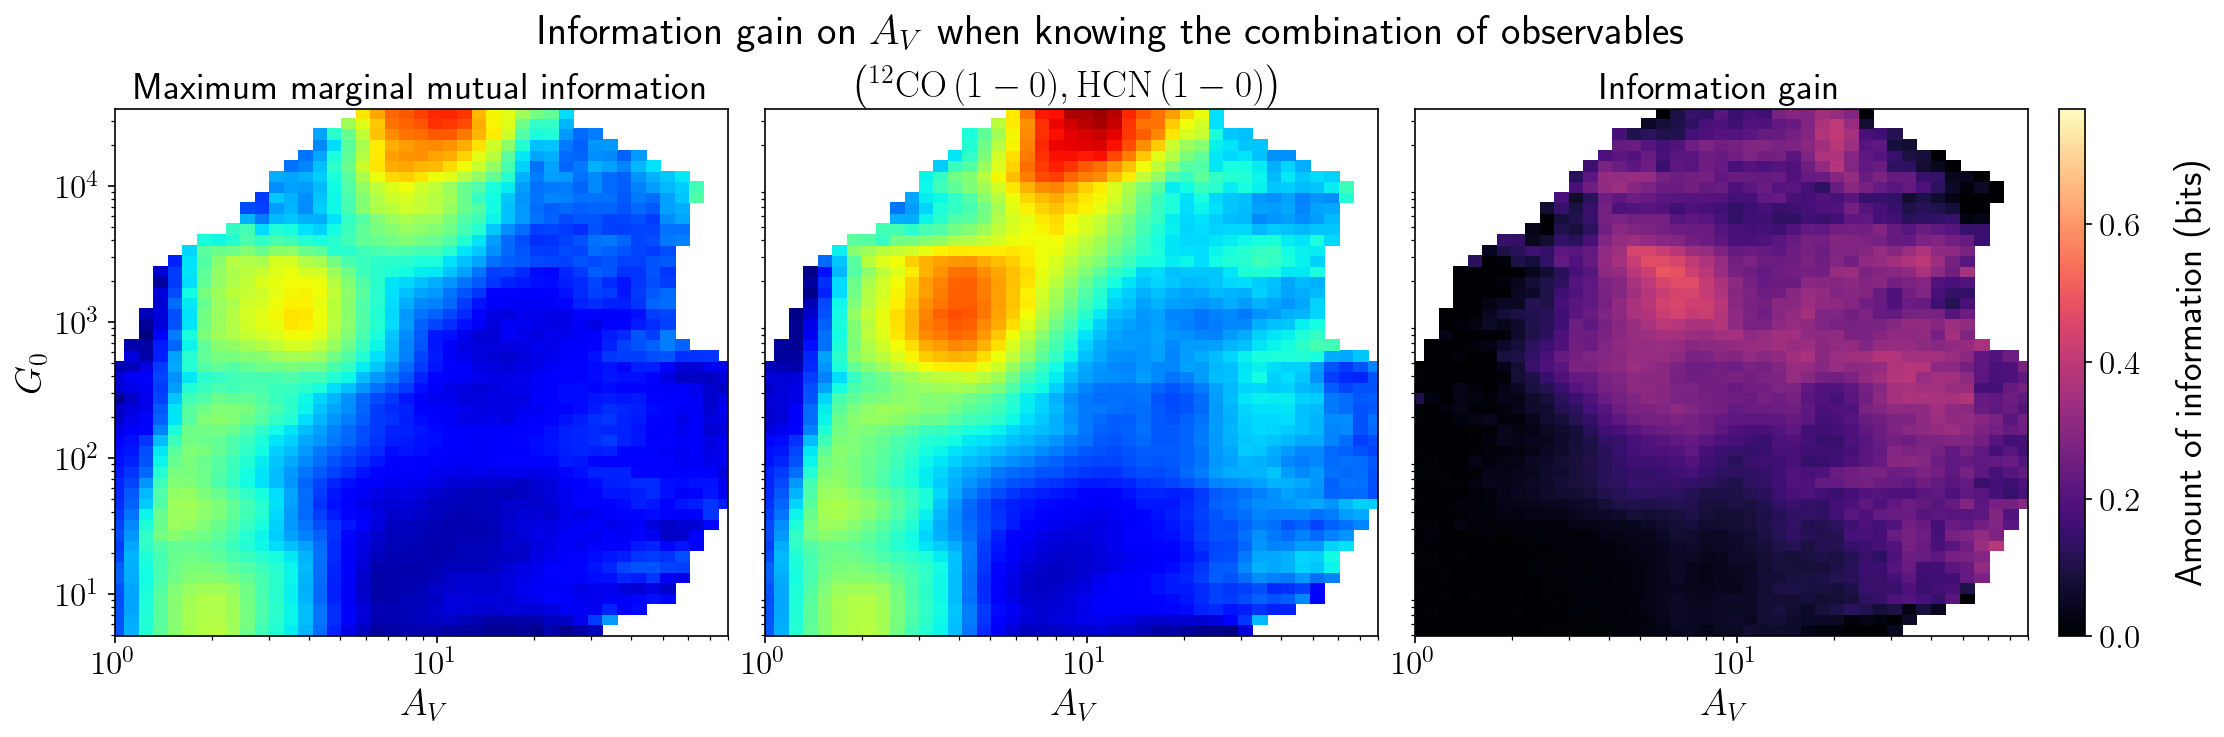
\includegraphics[width=0.95\linewidth]{../mi/av__12co10_hcn10_mi_gain.png}
    \end{figure}
\end{frame}

\begin{frame}{Informativity on $A_V$ of $\left(\mathrm{^{12}CO\,(1-0)},\mathrm{HCO^+\,(1-0)}\right)$}
    \begin{figure}
        \centering
        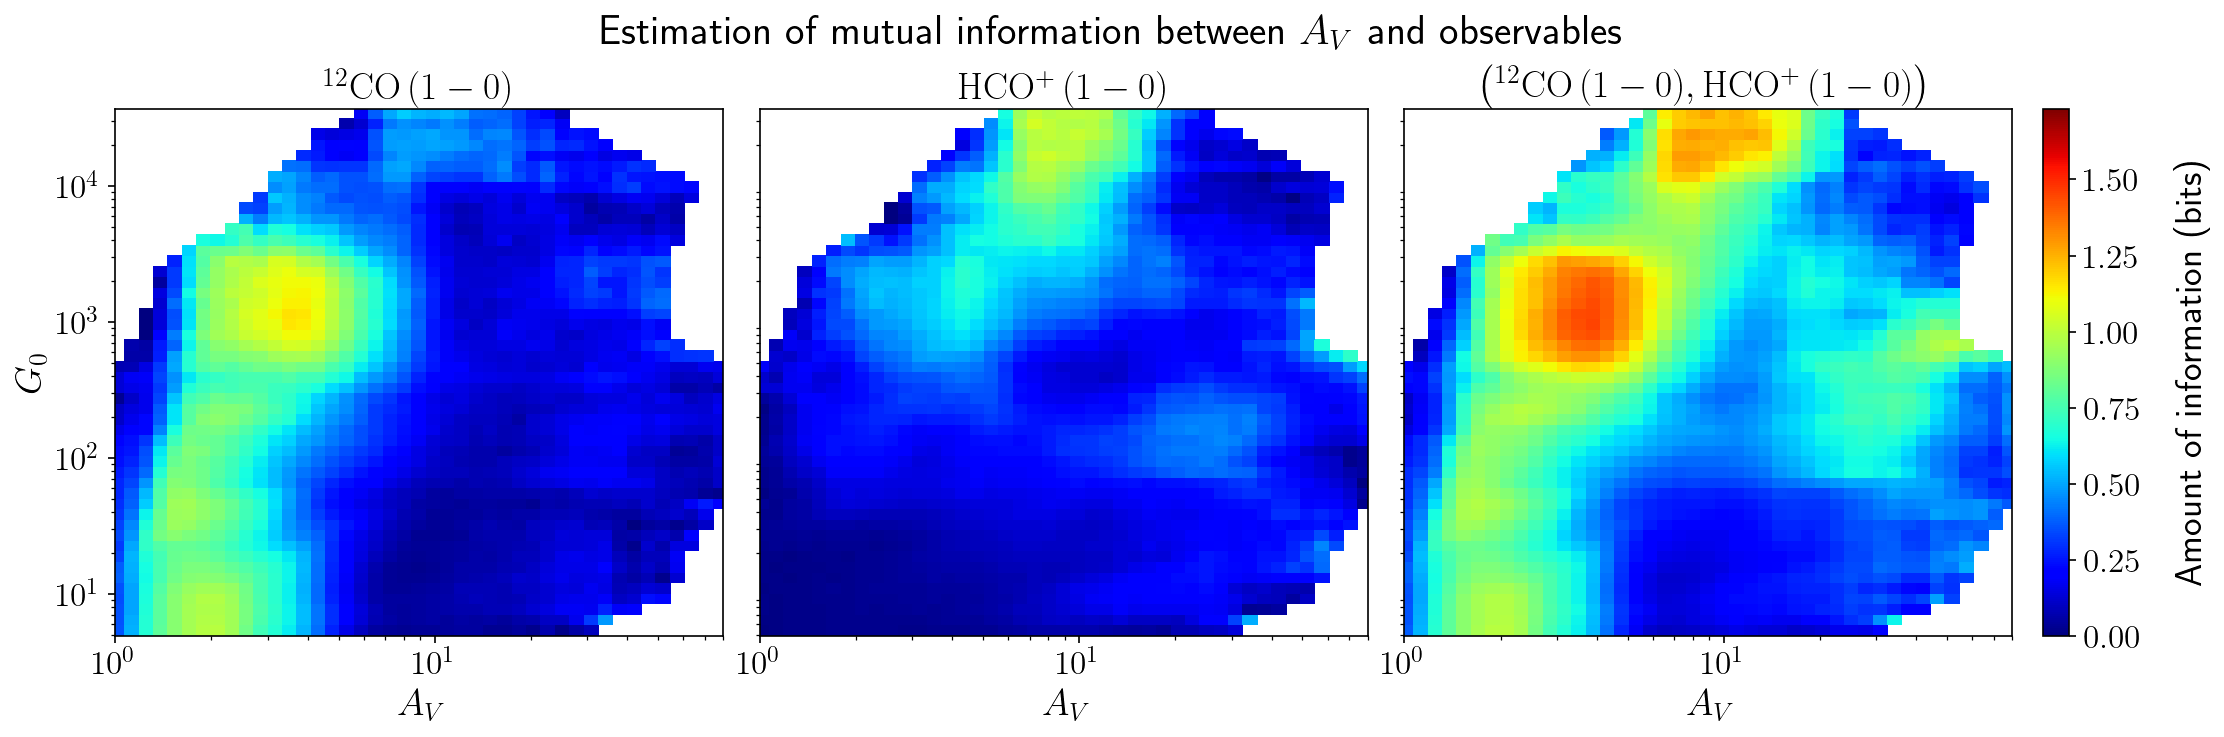
\includegraphics[width=0.95\linewidth]{../mi/av__12co10_hcop10_mi.png}
        \vfill
        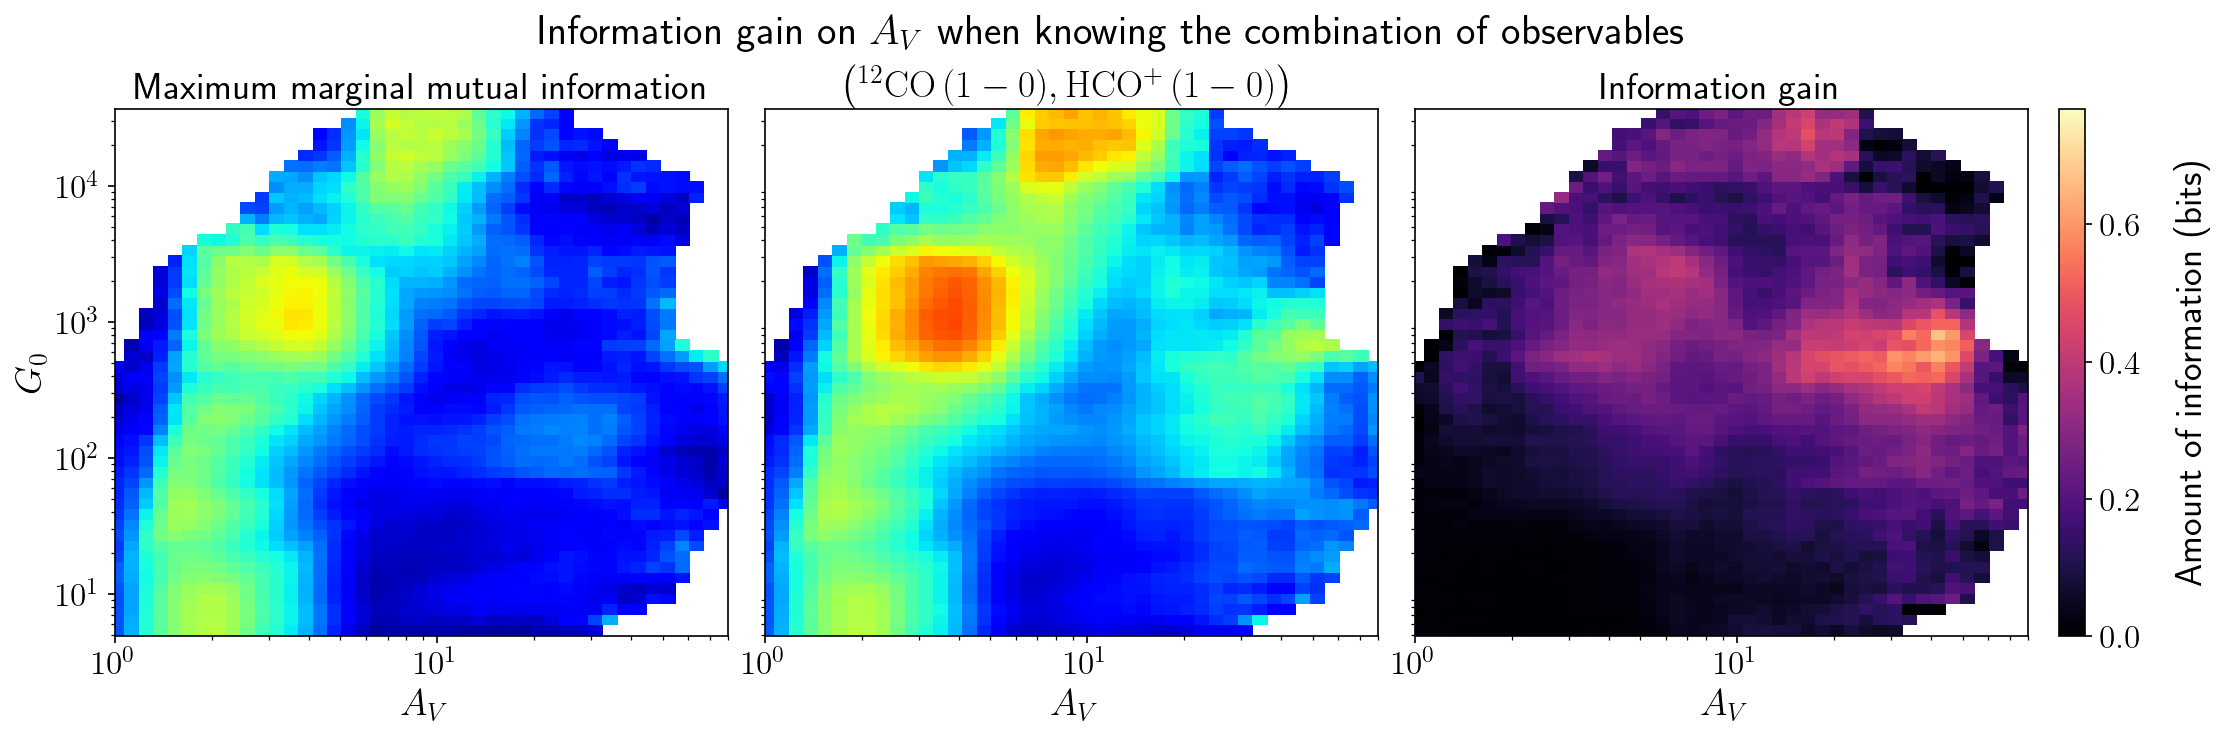
\includegraphics[width=0.95\linewidth]{../mi/av__12co10_hcop10_mi_gain.png}
    \end{figure}
\end{frame}

\begin{frame}{Informativity on $A_V$ of $\left(\mathrm{^{12}CO\,(1-0)},\mathrm{HNC\,(1-0)}\right)$}
    \begin{figure}
        \centering
        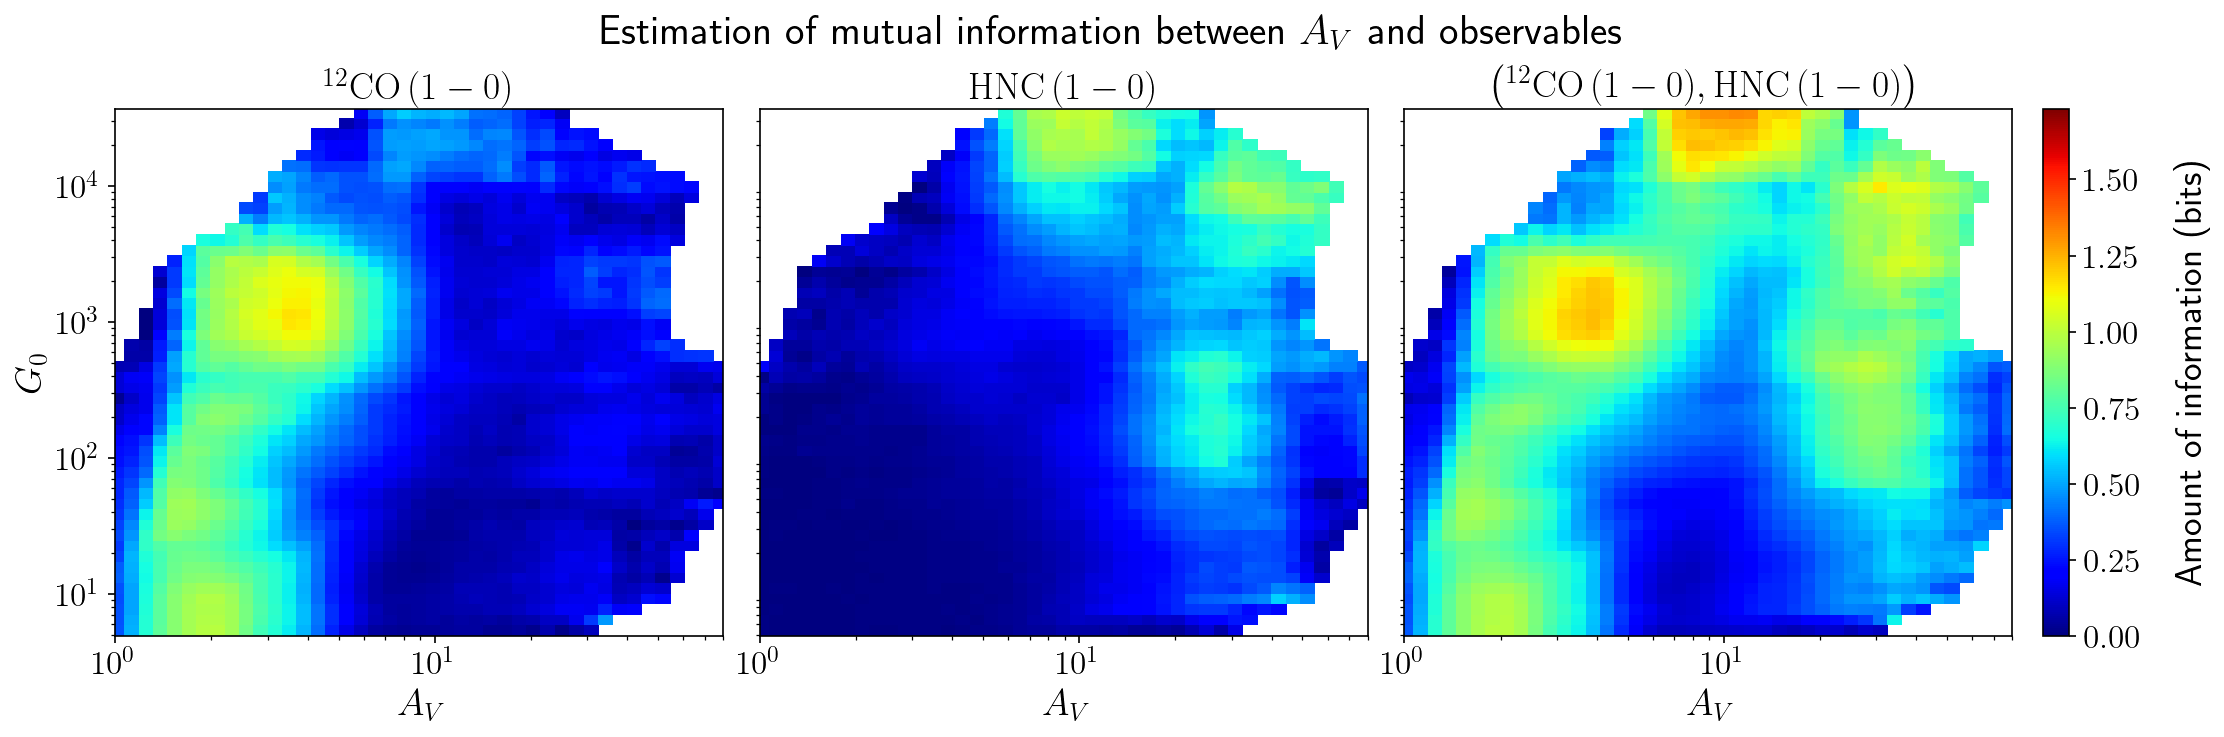
\includegraphics[width=0.95\linewidth]{../mi/av__12co10_hnc10_mi.png}
        \vfill
        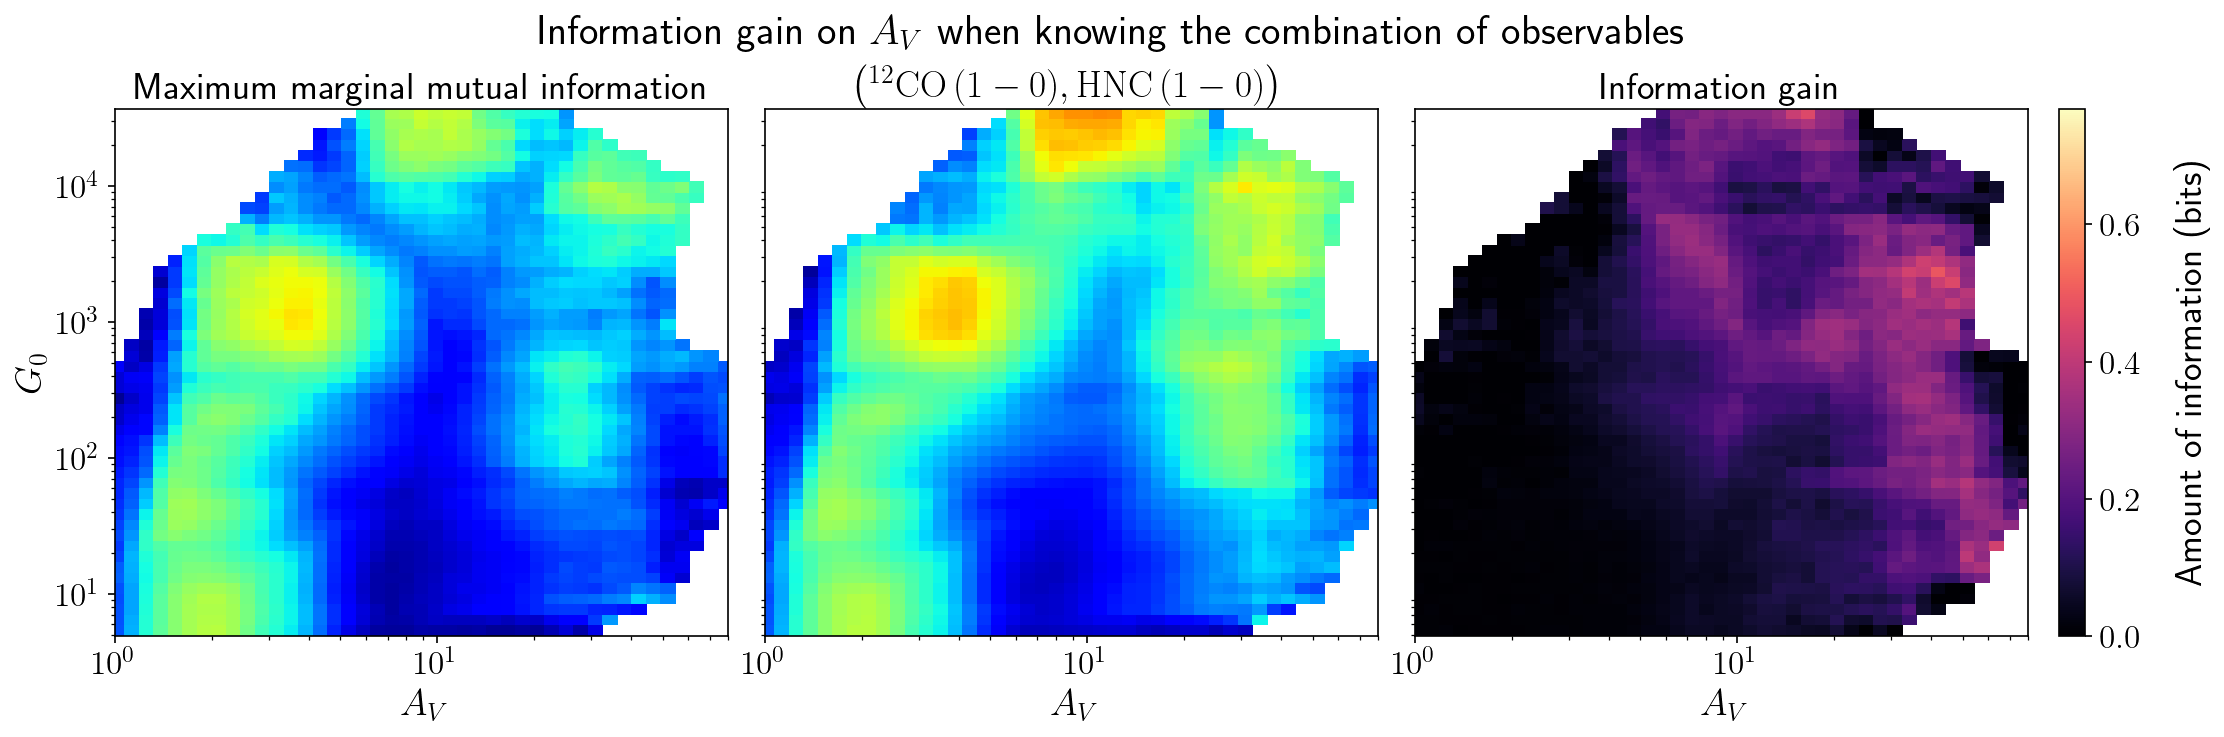
\includegraphics[width=0.95\linewidth]{../mi/av__12co10_hnc10_mi_gain.png}
    \end{figure}
\end{frame}

\begin{frame}{Informativity on $A_V$ of $\left(\mathrm{^{12}CO\,(1-0)},\mathrm{N_2H^+\,(1-0)}\right)$}
    \begin{figure}
        \centering
        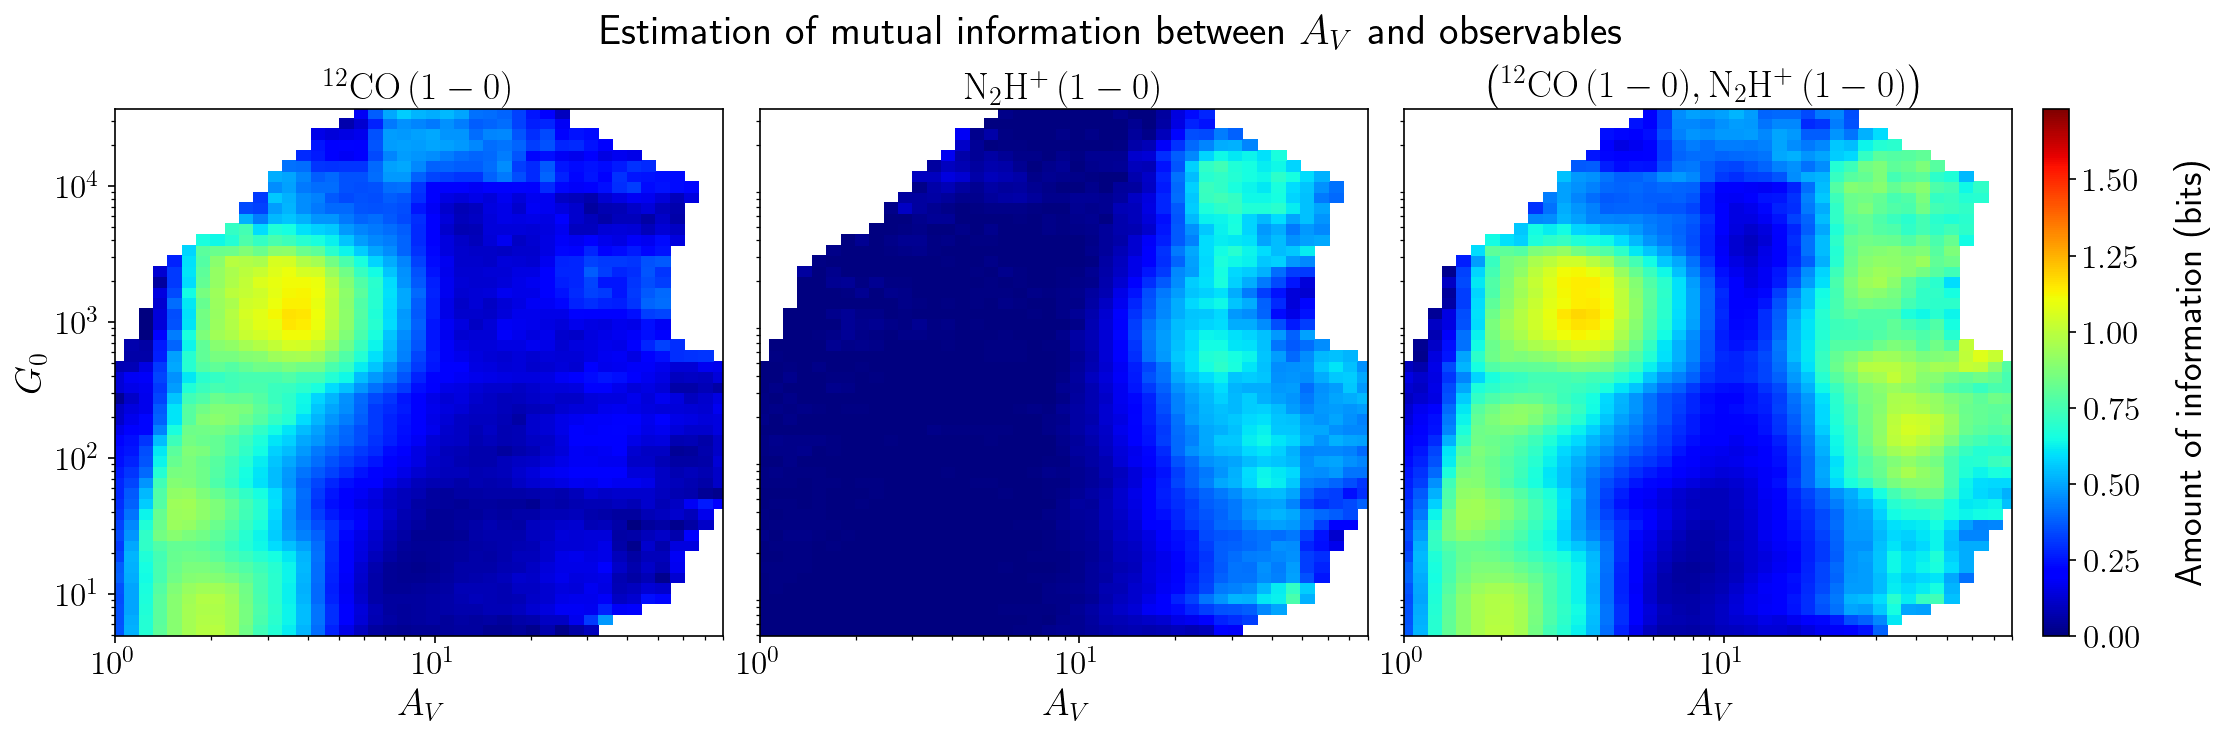
\includegraphics[width=0.95\linewidth]{../mi/av__12co10_n2hp10_mi.png}
        \vfill
        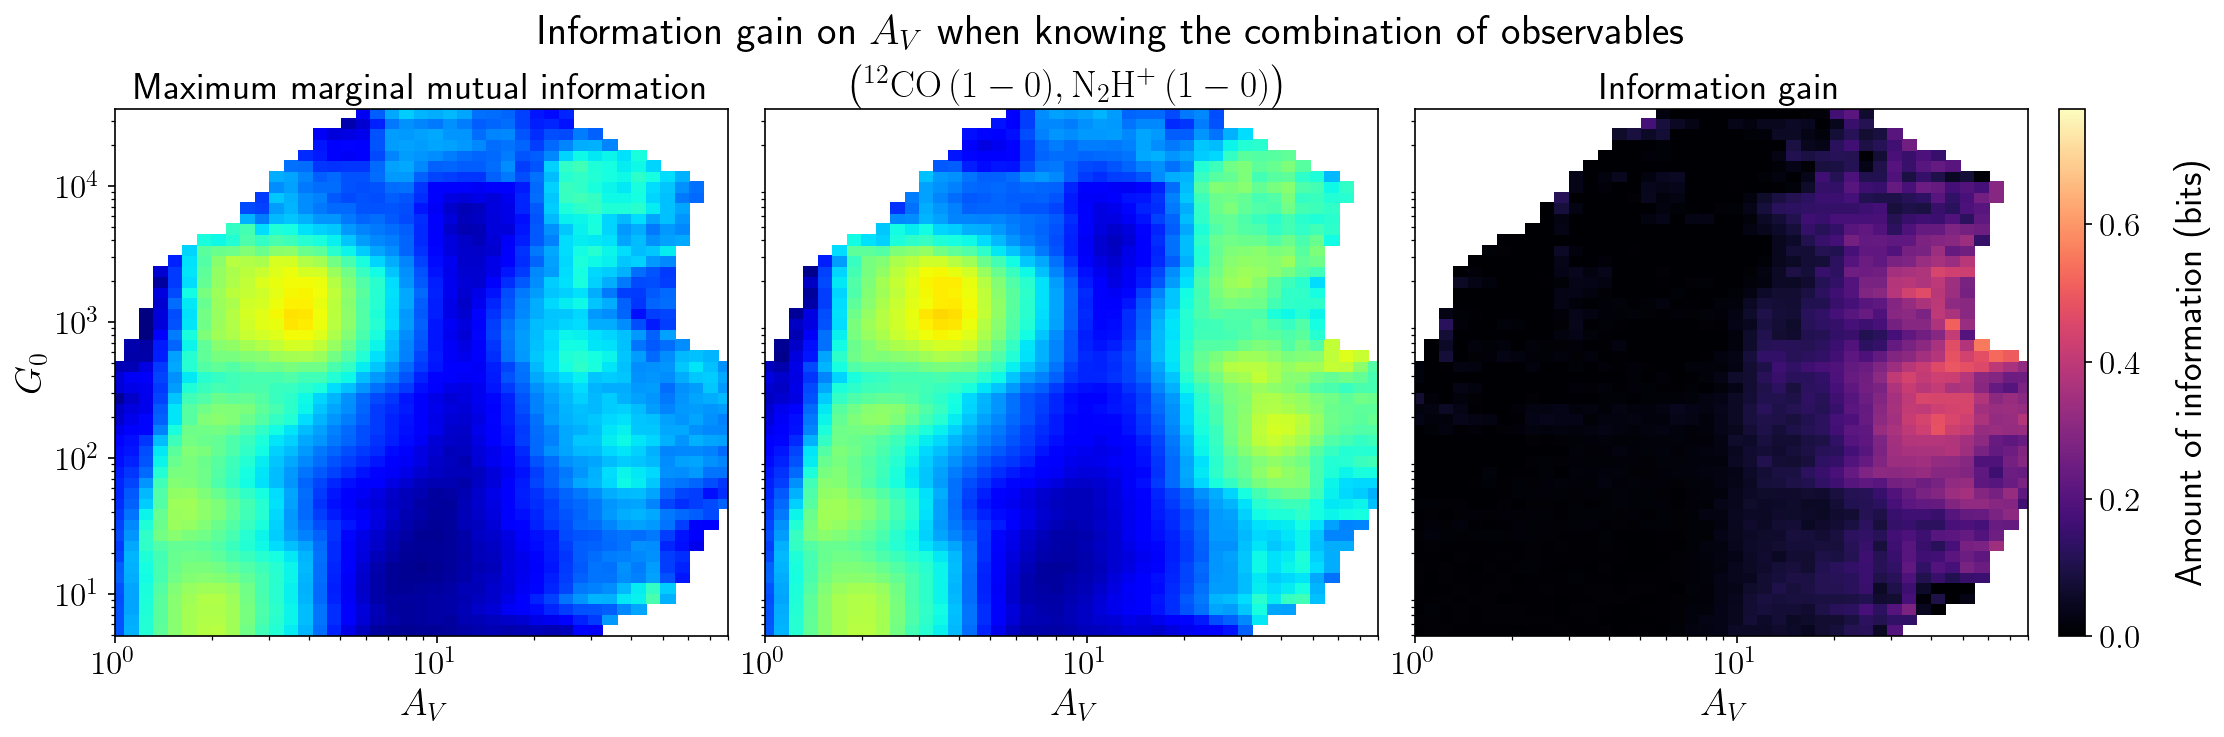
\includegraphics[width=0.95\linewidth]{../mi/av__12co10_n2hp10_mi_gain.png}
    \end{figure}
\end{frame}

\section{Combinations including $\mathrm{C^{18}O\,(1-0)}$ (11 available)}

\begin{frame}{Informativity on $A_V$ of $\left(\mathrm{^{12}CN\,(1-0)},\mathrm{C^{18}O\,(1-0)}\right)$}
    \begin{figure}
        \centering
        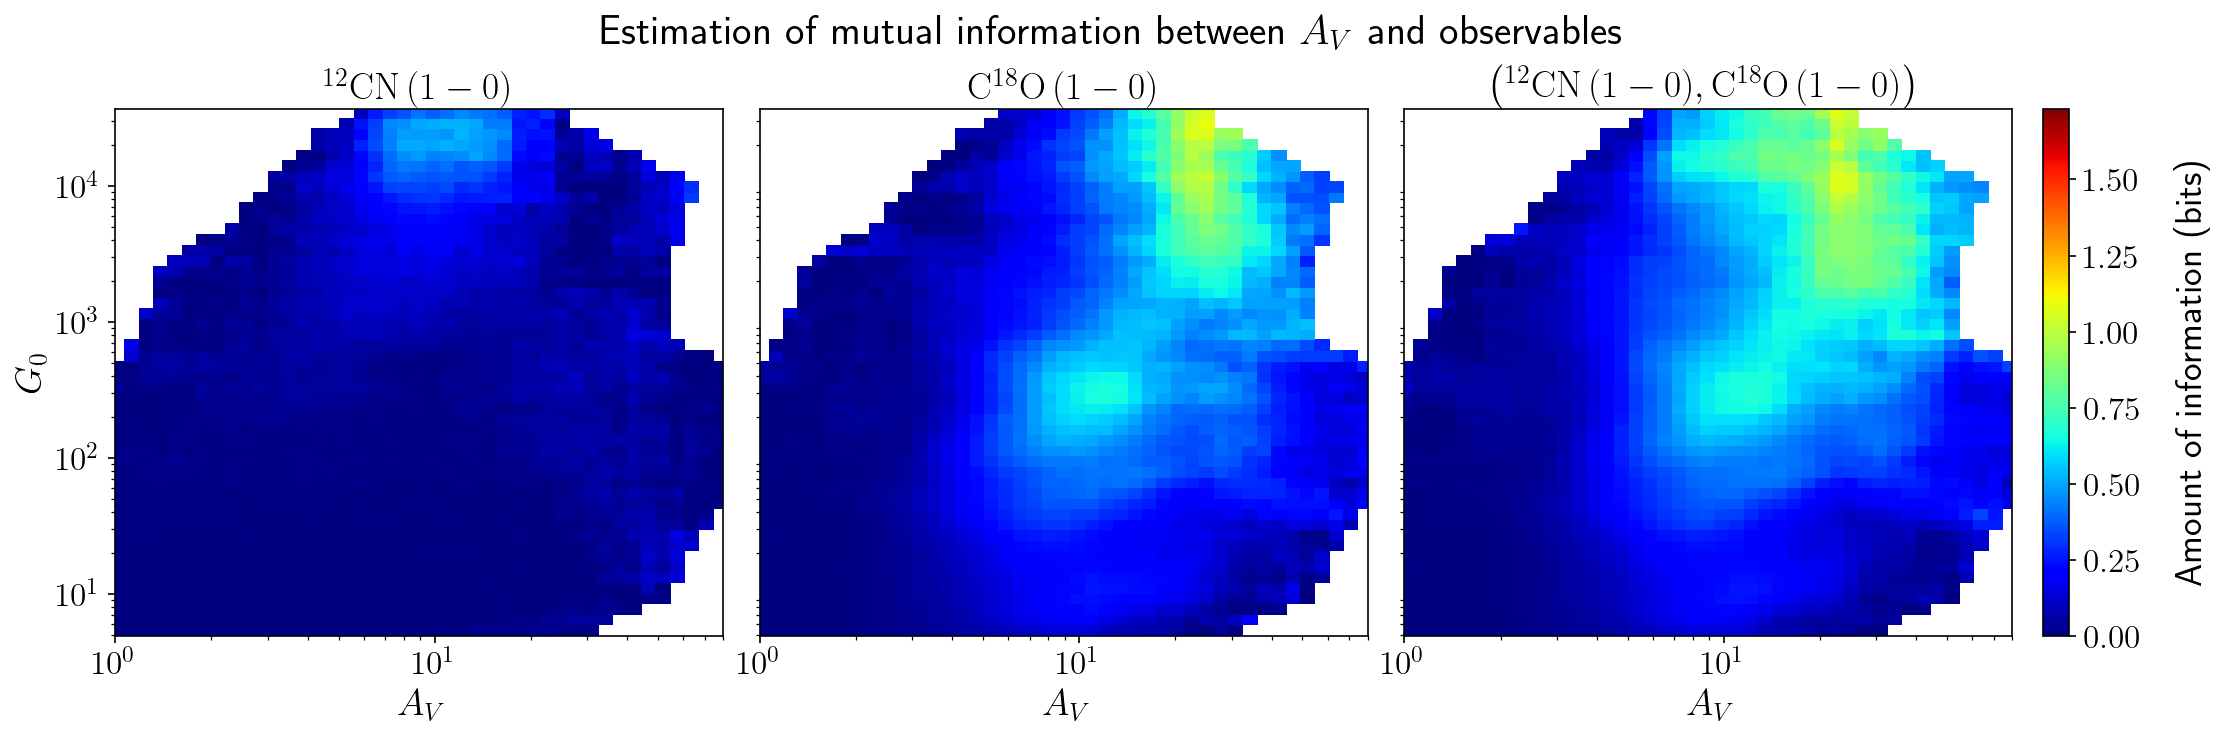
\includegraphics[width=0.95\linewidth]{../mi/av__12cn10_c18o10_mi.png}
        \vfill
        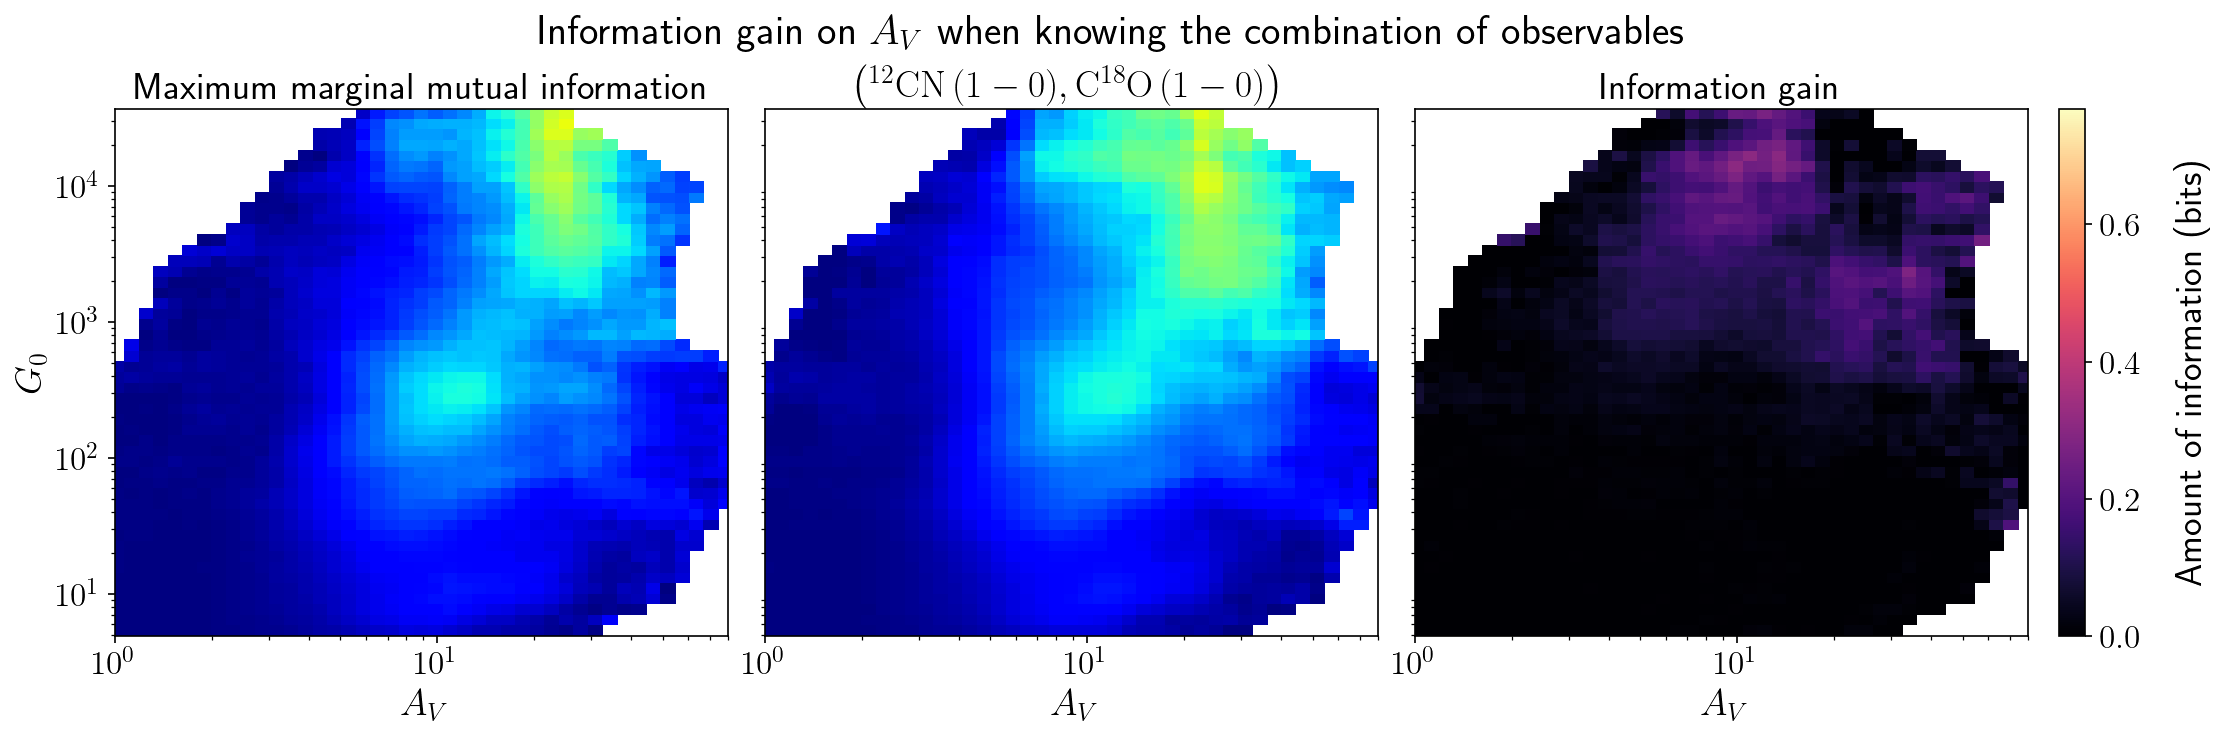
\includegraphics[width=0.95\linewidth]{../mi/av__12cn10_c18o10_mi_gain.png}
    \end{figure}
\end{frame}

\begin{frame}{Informativity on $A_V$ of $\left(\mathrm{^{12}CO\,(1-0)},\mathrm{C^{18}O\,(1-0)}\right)$}
    \begin{figure}
        \centering
        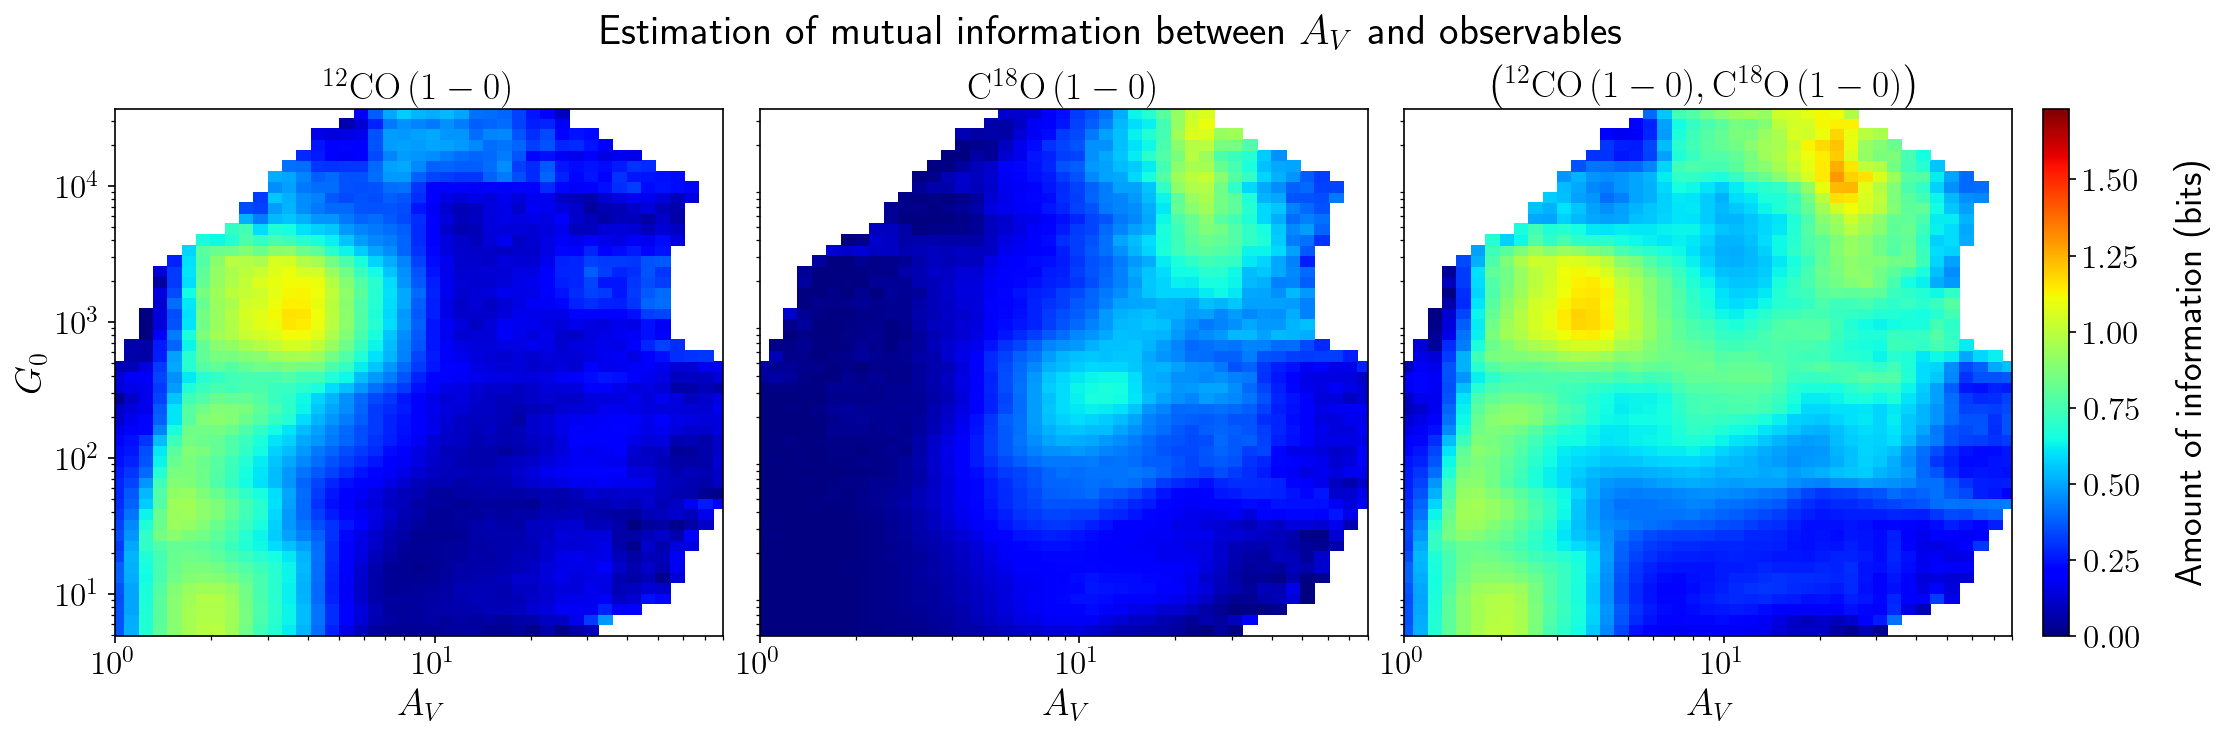
\includegraphics[width=0.95\linewidth]{../mi/av__12co10_c18o10_mi.png}
        \vfill
        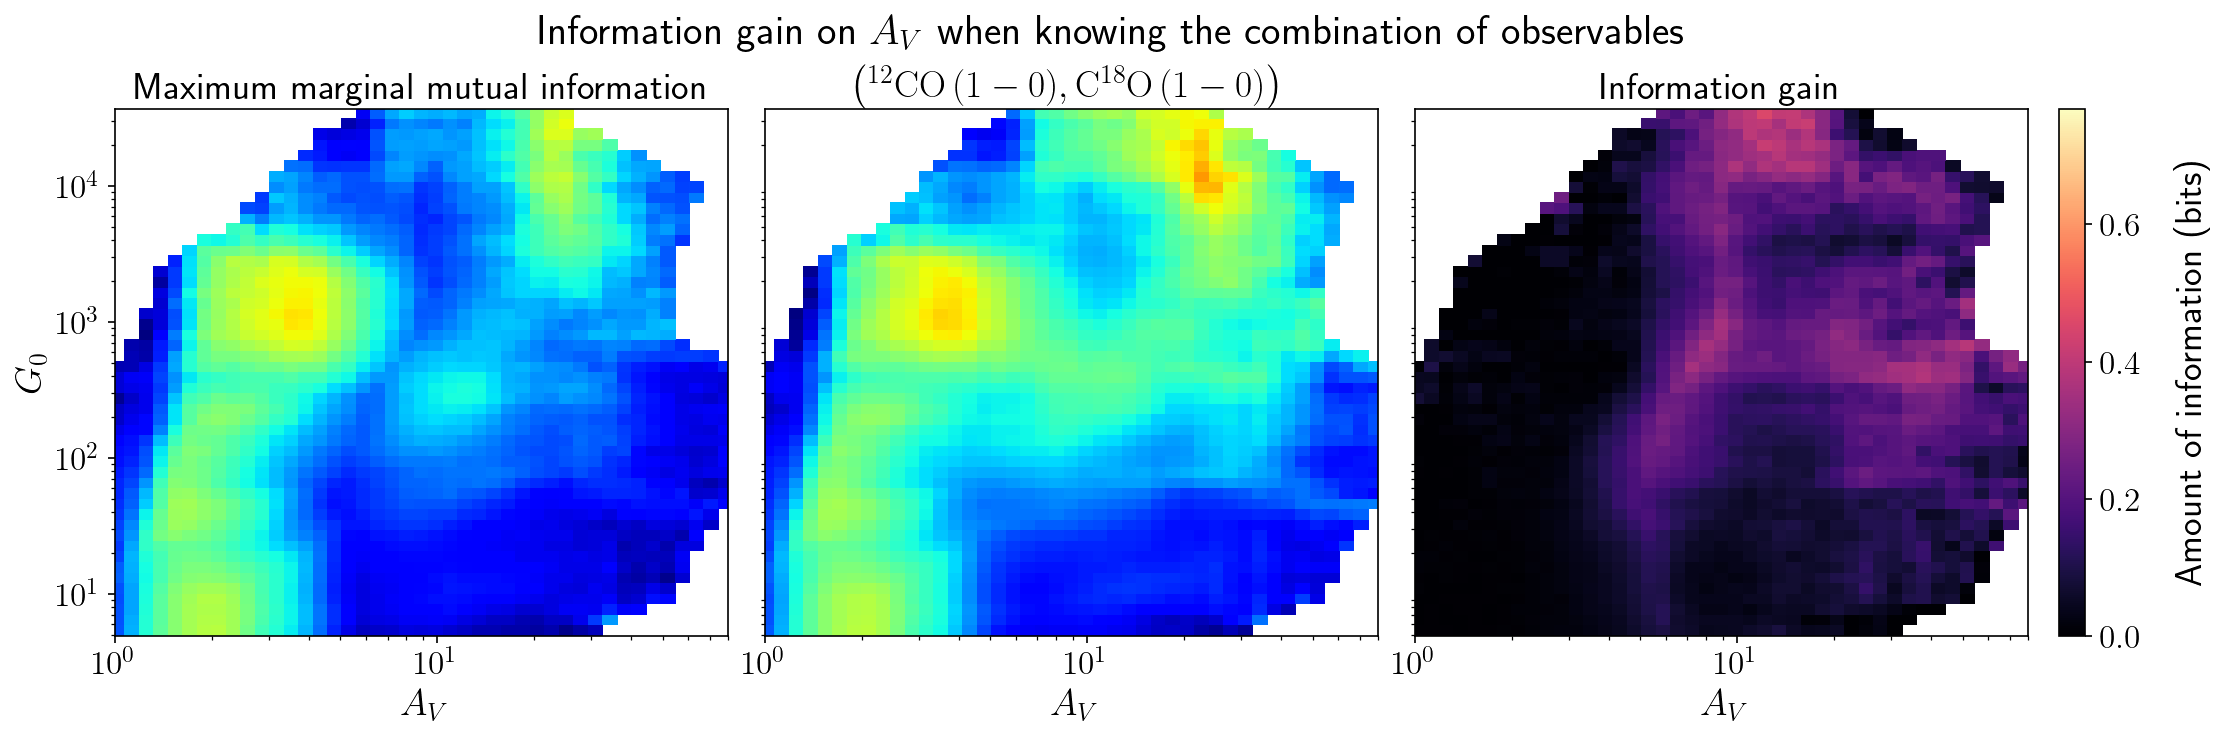
\includegraphics[width=0.95\linewidth]{../mi/av__12co10_c18o10_mi_gain.png}
    \end{figure}
\end{frame}

\begin{frame}{Informativity on $A_V$ of $\left(\mathrm{^{12}CS\,(2-1)},\mathrm{C^{18}O\,(1-0)}\right)$}
    \begin{figure}
        \centering
        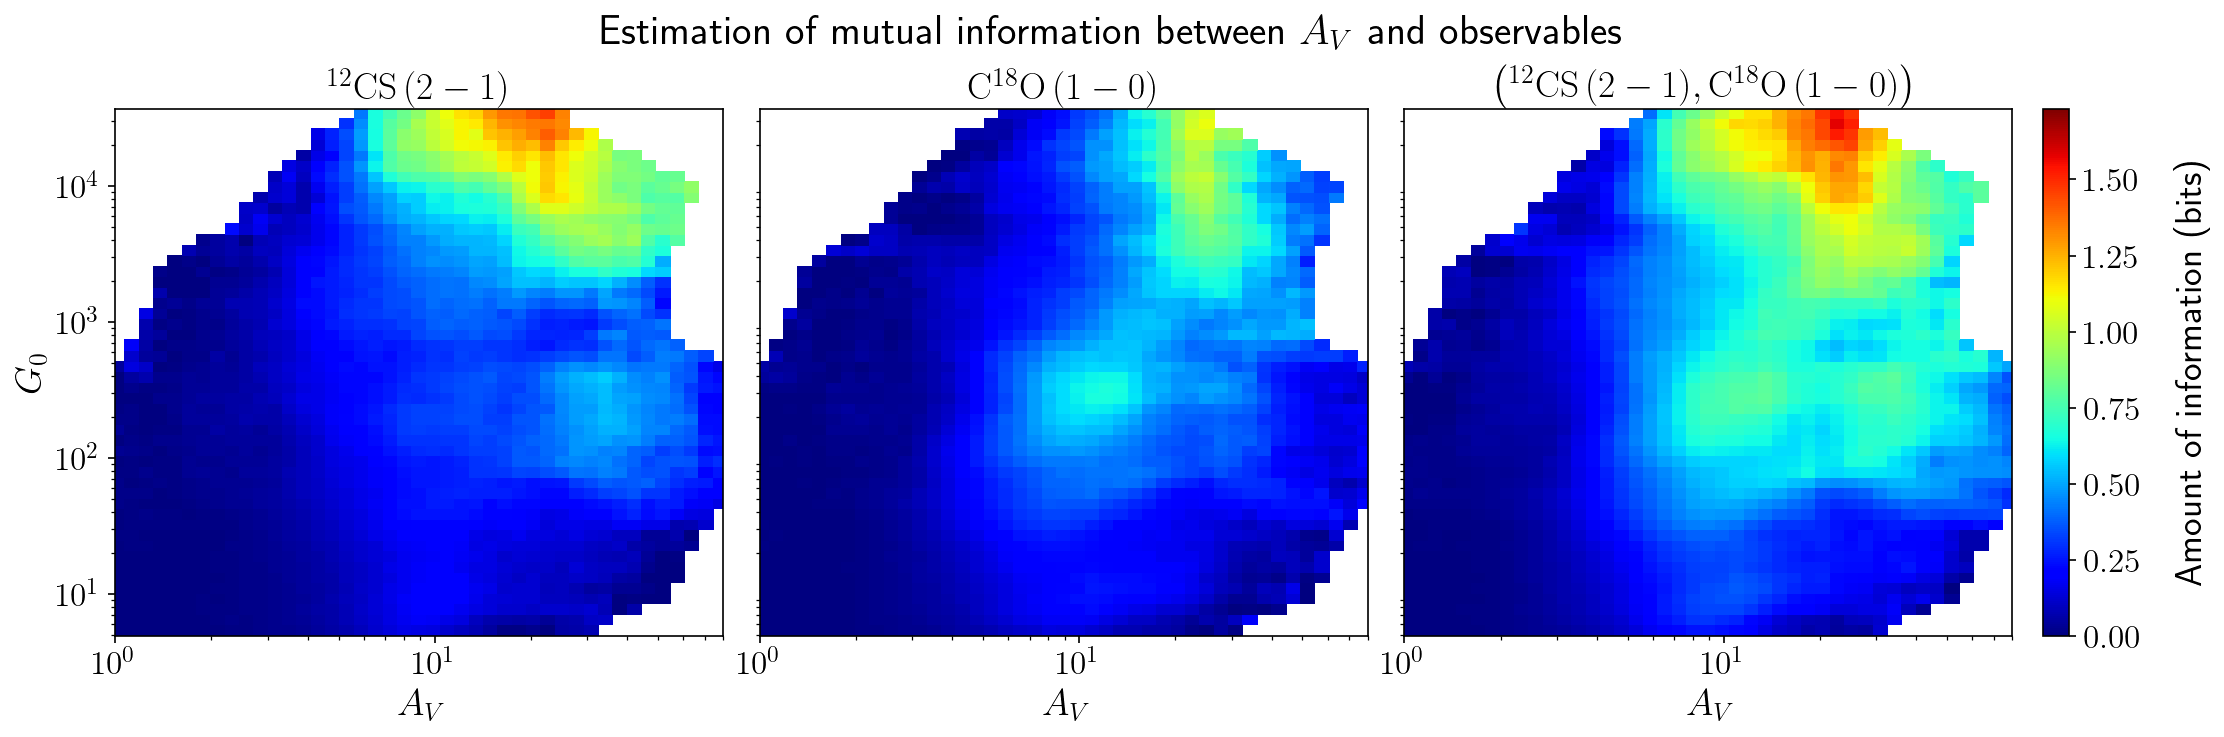
\includegraphics[width=0.95\linewidth]{../mi/av__12cs21_c18o10_mi.png}
        \vfill
        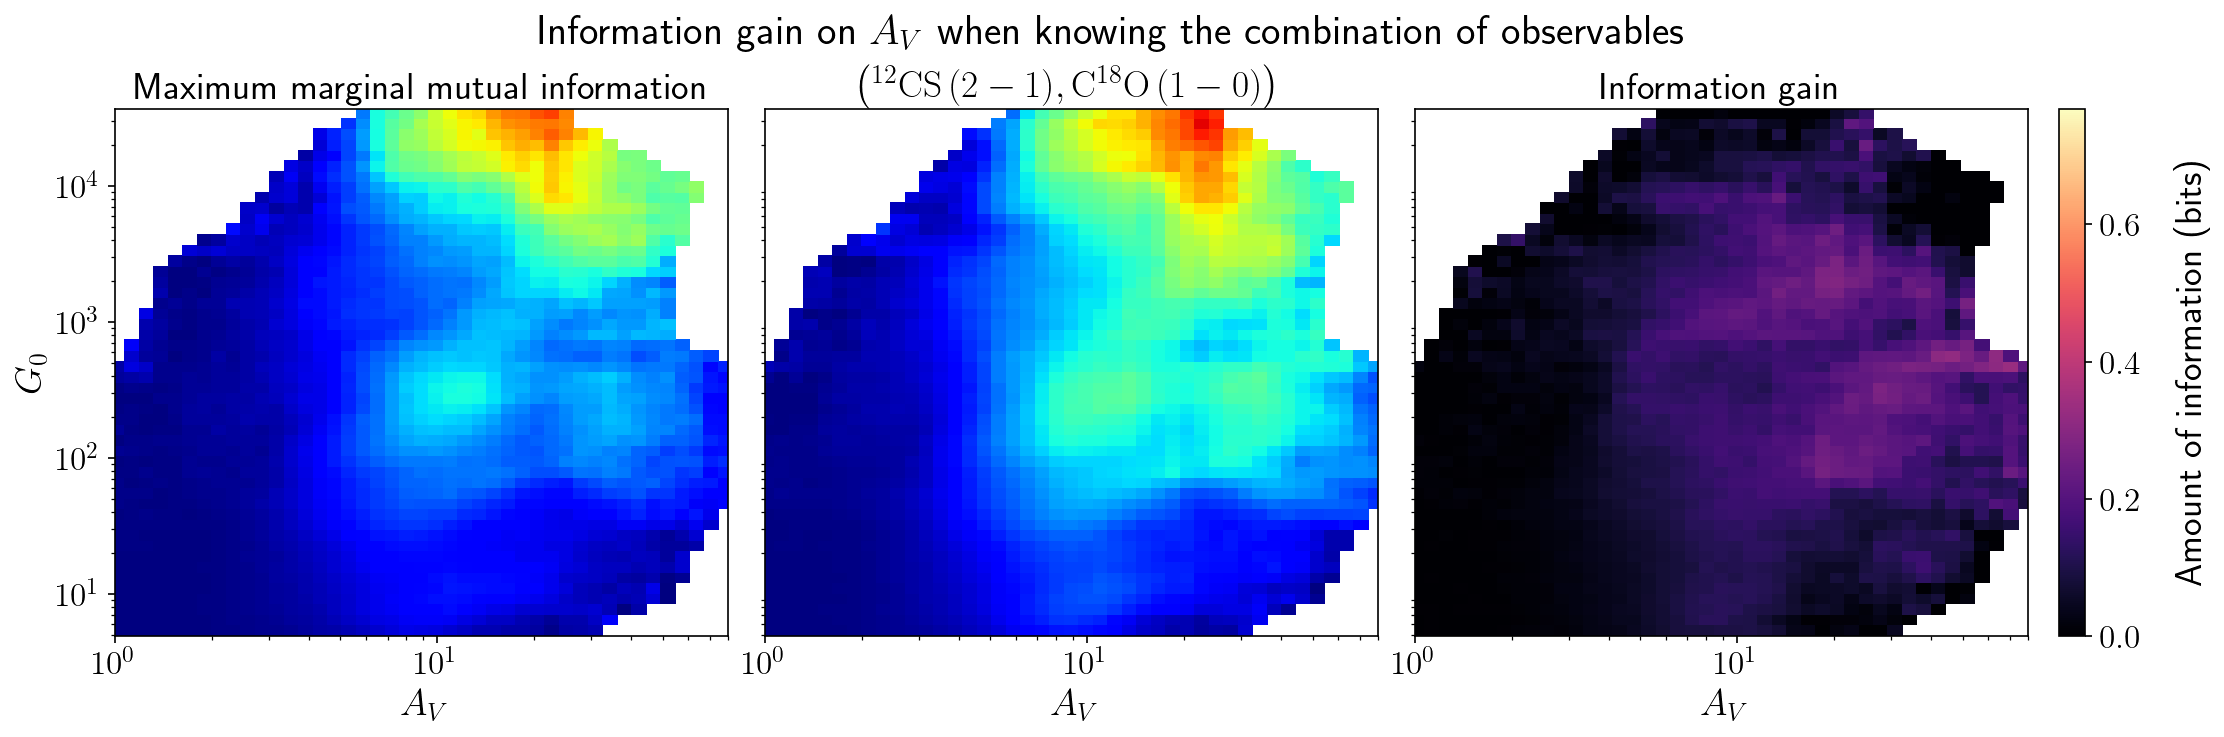
\includegraphics[width=0.95\linewidth]{../mi/av__12cs21_c18o10_mi_gain.png}
    \end{figure}
\end{frame}

\begin{frame}{Informativity on $A_V$ of $\left(\mathrm{^{13}CO\,(1-0)},\mathrm{C^{18}O\,(1-0)}\right)$}
    \begin{figure}
        \centering
        \includegraphics[width=0.95\linewidth]{../mi/av__13co10_c18o10_mi.png}
        \vfill
        \includegraphics[width=0.95\linewidth]{../mi/av__13co10_c18o10_mi_gain.png}
    \end{figure}
\end{frame}

\begin{frame}{Informativity on $A_V$ of $\left(\mathrm{^{32}SO\,(2-1)},\mathrm{C^{18}O\,(1-0)}\right)$}
    \begin{figure}
        \centering
        \includegraphics[width=0.95\linewidth]{../mi/av__32so21_c18o10_mi.png}
        \vfill
        \includegraphics[width=0.95\linewidth]{../mi/av__32so21_c18o10_mi_gain.png}
    \end{figure}
\end{frame}

\begin{frame}{Informativity on $A_V$ of $\left(\mathrm{C^{18}O\,(1-0)},\mathrm{CCH\,(1-0)}\right)$}
    \begin{figure}
        \centering
        \includegraphics[width=0.95\linewidth]{../mi/av__c18o10_cch10_mi.png}
        \vfill
        \includegraphics[width=0.95\linewidth]{../mi/av__c18o10_cch10_mi_gain.png}
    \end{figure}
\end{frame}

\begin{frame}{Informativity on $A_V$ of $\left(\mathrm{C^{18}O\,(1-0)},\mathrm{H_2CO}\right)$}
    \begin{figure}
        \centering
        \includegraphics[width=0.95\linewidth]{../mi/av__c18o10_h2co_mi.png}
        \vfill
        \includegraphics[width=0.95\linewidth]{../mi/av__c18o10_h2co_mi_gain.png}
    \end{figure}
\end{frame}

\begin{frame}{Informativity on $A_V$ of $\left(\mathrm{C^{18}O\,(1-0)},\mathrm{HCN\,(1-0)}\right)$}
    \begin{figure}
        \centering
        \includegraphics[width=0.95\linewidth]{../mi/av__c18o10_hcn10_mi.png}
        \vfill
        \includegraphics[width=0.95\linewidth]{../mi/av__c18o10_hcn10_mi_gain.png}
    \end{figure}
\end{frame}

\begin{frame}{Informativity on $A_V$ of $\left(\mathrm{C^{18}O\,(1-0)},\mathrm{HCO^+\,(1-0)}\right)$}
    \begin{figure}
        \centering
        \includegraphics[width=0.95\linewidth]{../mi/av__c18o10_hcop10_mi.png}
        \vfill
        \includegraphics[width=0.95\linewidth]{../mi/av__c18o10_hcop10_mi_gain.png}
    \end{figure}
\end{frame}

\begin{frame}{Informativity on $A_V$ of $\left(\mathrm{C^{18}O\,(1-0)},\mathrm{HNC\,(1-0)}\right)$}
    \begin{figure}
        \centering
        \includegraphics[width=0.95\linewidth]{../mi/av__c18o10_hnc10_mi.png}
        \vfill
        \includegraphics[width=0.95\linewidth]{../mi/av__c18o10_hnc10_mi_gain.png}
    \end{figure}
\end{frame}

\begin{frame}{Informativity on $A_V$ of $\left(\mathrm{C^{18}O\,(1-0)},\mathrm{N_2H^+\,(1-0)}\right)$}
    \begin{figure}
        \centering
        \includegraphics[width=0.95\linewidth]{../mi/av__c18o10_n2hp10_mi.png}
        \vfill
        \includegraphics[width=0.95\linewidth]{../mi/av__c18o10_n2hp10_mi_gain.png}
    \end{figure}
\end{frame}

\section{Combinations including $\mathrm{^{32}SO\,(2-1)}$ (11 available)}

\begin{frame}{Informativity on $A_V$ of $\left(\mathrm{^{12}CN\,(1-0)},\mathrm{^{32}SO\,(2-1)}\right)$}
    \begin{figure}
        \centering
        \includegraphics[width=0.95\linewidth]{../mi/av__12cn10_32so21_mi.png}
        \vfill
        \includegraphics[width=0.95\linewidth]{../mi/av__12cn10_32so21_mi_gain.png}
    \end{figure}
\end{frame}

\begin{frame}{Informativity on $A_V$ of $\left(\mathrm{^{12}CO\,(1-0)},\mathrm{^{32}SO\,(2-1)}\right)$}
    \begin{figure}
        \centering
        \includegraphics[width=0.95\linewidth]{../mi/av__12co10_32so21_mi.png}
        \vfill
        \includegraphics[width=0.95\linewidth]{../mi/av__12co10_32so21_mi_gain.png}
    \end{figure}
\end{frame}

\begin{frame}{Informativity on $A_V$ of $\left(\mathrm{^{12}CS\,(2-1)},\mathrm{^{32}SO\,(2-1)}\right)$}
    \begin{figure}
        \centering
        \includegraphics[width=0.95\linewidth]{../mi/av__12cs21_32so21_mi.png}
        \vfill
        \includegraphics[width=0.95\linewidth]{../mi/av__12cs21_32so21_mi_gain.png}
    \end{figure}
\end{frame}

\begin{frame}{Informativity on $A_V$ of $\left(\mathrm{^{13}CO\,(1-0)},\mathrm{^{32}SO\,(2-1)}\right)$}
    \begin{figure}
        \centering
        \includegraphics[width=0.95\linewidth]{../mi/av__13co10_32so21_mi.png}
        \vfill
        \includegraphics[width=0.95\linewidth]{../mi/av__13co10_32so21_mi_gain.png}
    \end{figure}
\end{frame}

\begin{frame}{Informativity on $A_V$ of $\left(\mathrm{^{32}SO\,(2-1)},\mathrm{C^{18}O\,(1-0)}\right)$}
    \begin{figure}
        \centering
        \includegraphics[width=0.95\linewidth]{../mi/av__32so21_c18o10_mi.png}
        \vfill
        \includegraphics[width=0.95\linewidth]{../mi/av__32so21_c18o10_mi_gain.png}
    \end{figure}
\end{frame}

\begin{frame}{Informativity on $A_V$ of $\left(\mathrm{^{32}SO\,(2-1)},\mathrm{CCH\,(1-0)}\right)$}
    \begin{figure}
        \centering
        \includegraphics[width=0.95\linewidth]{../mi/av__32so21_cch10_mi.png}
        \vfill
        \includegraphics[width=0.95\linewidth]{../mi/av__32so21_cch10_mi_gain.png}
    \end{figure}
\end{frame}

\begin{frame}{Informativity on $A_V$ of $\left(\mathrm{^{32}SO\,(2-1)},\mathrm{H_2CO}\right)$}
    \begin{figure}
        \centering
        \includegraphics[width=0.95\linewidth]{../mi/av__32so21_h2co_mi.png}
        \vfill
        \includegraphics[width=0.95\linewidth]{../mi/av__32so21_h2co_mi_gain.png}
    \end{figure}
\end{frame}

\begin{frame}{Informativity on $A_V$ of $\left(\mathrm{^{32}SO\,(2-1)},\mathrm{HCN\,(1-0)}\right)$}
    \begin{figure}
        \centering
        \includegraphics[width=0.95\linewidth]{../mi/av__32so21_hcn10_mi.png}
        \vfill
        \includegraphics[width=0.95\linewidth]{../mi/av__32so21_hcn10_mi_gain.png}
    \end{figure}
\end{frame}

\begin{frame}{Informativity on $A_V$ of $\left(\mathrm{^{32}SO\,(2-1)},\mathrm{HCO^+\,(1-0)}\right)$}
    \begin{figure}
        \centering
        \includegraphics[width=0.95\linewidth]{../mi/av__32so21_hcop10_mi.png}
        \vfill
        \includegraphics[width=0.95\linewidth]{../mi/av__32so21_hcop10_mi_gain.png}
    \end{figure}
\end{frame}

\begin{frame}{Informativity on $A_V$ of $\left(\mathrm{^{32}SO\,(2-1)},\mathrm{HNC\,(1-0)}\right)$}
    \begin{figure}
        \centering
        \includegraphics[width=0.95\linewidth]{../mi/av__32so21_hnc10_mi.png}
        \vfill
        \includegraphics[width=0.95\linewidth]{../mi/av__32so21_hnc10_mi_gain.png}
    \end{figure}
\end{frame}

\begin{frame}{Informativity on $A_V$ of $\left(\mathrm{^{32}SO\,(2-1)},\mathrm{N_2H^+\,(1-0)}\right)$}
    \begin{figure}
        \centering
        \includegraphics[width=0.95\linewidth]{../mi/av__32so21_n2hp10_mi.png}
        \vfill
        \includegraphics[width=0.95\linewidth]{../mi/av__32so21_n2hp10_mi_gain.png}
    \end{figure}
\end{frame}

\section{Combinations including $\mathrm{^{12}CN\,(1-0)}$ (11 available)}

\begin{frame}{Informativity on $A_V$ of $\left(\mathrm{^{12}CN\,(1-0)},\mathrm{^{12}CO\,(1-0)}\right)$}
    \begin{figure}
        \centering
        \includegraphics[width=0.95\linewidth]{../mi/av__12cn10_12co10_mi.png}
        \vfill
        \includegraphics[width=0.95\linewidth]{../mi/av__12cn10_12co10_mi_gain.png}
    \end{figure}
\end{frame}

\begin{frame}{Informativity on $A_V$ of $\left(\mathrm{^{12}CN\,(1-0)},\mathrm{^{12}CS\,(2-1)}\right)$}
    \begin{figure}
        \centering
        \includegraphics[width=0.95\linewidth]{../mi/av__12cn10_12cs21_mi.png}
        \vfill
        \includegraphics[width=0.95\linewidth]{../mi/av__12cn10_12cs21_mi_gain.png}
    \end{figure}
\end{frame}

\begin{frame}{Informativity on $A_V$ of $\left(\mathrm{^{12}CN\,(1-0)},\mathrm{^{13}CO\,(1-0)}\right)$}
    \begin{figure}
        \centering
        \includegraphics[width=0.95\linewidth]{../mi/av__12cn10_13co10_mi.png}
        \vfill
        \includegraphics[width=0.95\linewidth]{../mi/av__12cn10_13co10_mi_gain.png}
    \end{figure}
\end{frame}

\begin{frame}{Informativity on $A_V$ of $\left(\mathrm{^{12}CN\,(1-0)},\mathrm{^{32}SO\,(2-1)}\right)$}
    \begin{figure}
        \centering
        \includegraphics[width=0.95\linewidth]{../mi/av__12cn10_32so21_mi.png}
        \vfill
        \includegraphics[width=0.95\linewidth]{../mi/av__12cn10_32so21_mi_gain.png}
    \end{figure}
\end{frame}

\begin{frame}{Informativity on $A_V$ of $\left(\mathrm{^{12}CN\,(1-0)},\mathrm{C^{18}O\,(1-0)}\right)$}
    \begin{figure}
        \centering
        \includegraphics[width=0.95\linewidth]{../mi/av__12cn10_c18o10_mi.png}
        \vfill
        \includegraphics[width=0.95\linewidth]{../mi/av__12cn10_c18o10_mi_gain.png}
    \end{figure}
\end{frame}

\begin{frame}{Informativity on $A_V$ of $\left(\mathrm{^{12}CN\,(1-0)},\mathrm{CCH\,(1-0)}\right)$}
    \begin{figure}
        \centering
        \includegraphics[width=0.95\linewidth]{../mi/av__12cn10_cch10_mi.png}
        \vfill
        \includegraphics[width=0.95\linewidth]{../mi/av__12cn10_cch10_mi_gain.png}
    \end{figure}
\end{frame}

\begin{frame}{Informativity on $A_V$ of $\left(\mathrm{^{12}CN\,(1-0)},\mathrm{H_2CO}\right)$}
    \begin{figure}
        \centering
        \includegraphics[width=0.95\linewidth]{../mi/av__12cn10_h2co_mi.png}
        \vfill
        \includegraphics[width=0.95\linewidth]{../mi/av__12cn10_h2co_mi_gain.png}
    \end{figure}
\end{frame}

\begin{frame}{Informativity on $A_V$ of $\left(\mathrm{^{12}CN\,(1-0)},\mathrm{HCN\,(1-0)}\right)$}
    \begin{figure}
        \centering
        \includegraphics[width=0.95\linewidth]{../mi/av__12cn10_hcn10_mi.png}
        \vfill
        \includegraphics[width=0.95\linewidth]{../mi/av__12cn10_hcn10_mi_gain.png}
    \end{figure}
\end{frame}

\begin{frame}{Informativity on $A_V$ of $\left(\mathrm{^{12}CN\,(1-0)},\mathrm{HCO^+\,(1-0)}\right)$}
    \begin{figure}
        \centering
        \includegraphics[width=0.95\linewidth]{../mi/av__12cn10_hcop10_mi.png}
        \vfill
        \includegraphics[width=0.95\linewidth]{../mi/av__12cn10_hcop10_mi_gain.png}
    \end{figure}
\end{frame}

\begin{frame}{Informativity on $A_V$ of $\left(\mathrm{^{12}CN\,(1-0)},\mathrm{HNC\,(1-0)}\right)$}
    \begin{figure}
        \centering
        \includegraphics[width=0.95\linewidth]{../mi/av__12cn10_hnc10_mi.png}
        \vfill
        \includegraphics[width=0.95\linewidth]{../mi/av__12cn10_hnc10_mi_gain.png}
    \end{figure}
\end{frame}

\begin{frame}{Informativity on $A_V$ of $\left(\mathrm{^{12}CN\,(1-0)},\mathrm{N_2H^+\,(1-0)}\right)$}
    \begin{figure}
        \centering
        \includegraphics[width=0.95\linewidth]{../mi/av__12cn10_n2hp10_mi.png}
        \vfill
        \includegraphics[width=0.95\linewidth]{../mi/av__12cn10_n2hp10_mi_gain.png}
    \end{figure}
\end{frame}

\section{Combinations including $\mathrm{N_2H^+\,(1-0)}$ (11 available)}

\begin{frame}{Informativity on $A_V$ of $\left(\mathrm{^{12}CN\,(1-0)},\mathrm{N_2H^+\,(1-0)}\right)$}
    \begin{figure}
        \centering
        \includegraphics[width=0.95\linewidth]{../mi/av__12cn10_n2hp10_mi.png}
        \vfill
        \includegraphics[width=0.95\linewidth]{../mi/av__12cn10_n2hp10_mi_gain.png}
    \end{figure}
\end{frame}

\begin{frame}{Informativity on $A_V$ of $\left(\mathrm{^{12}CO\,(1-0)},\mathrm{N_2H^+\,(1-0)}\right)$}
    \begin{figure}
        \centering
        \includegraphics[width=0.95\linewidth]{../mi/av__12co10_n2hp10_mi.png}
        \vfill
        \includegraphics[width=0.95\linewidth]{../mi/av__12co10_n2hp10_mi_gain.png}
    \end{figure}
\end{frame}

\begin{frame}{Informativity on $A_V$ of $\left(\mathrm{^{12}CS\,(2-1)},\mathrm{N_2H^+\,(1-0)}\right)$}
    \begin{figure}
        \centering
        \includegraphics[width=0.95\linewidth]{../mi/av__12cs21_n2hp10_mi.png}
        \vfill
        \includegraphics[width=0.95\linewidth]{../mi/av__12cs21_n2hp10_mi_gain.png}
    \end{figure}
\end{frame}

\begin{frame}{Informativity on $A_V$ of $\left(\mathrm{^{13}CO\,(1-0)},\mathrm{N_2H^+\,(1-0)}\right)$}
    \begin{figure}
        \centering
        \includegraphics[width=0.95\linewidth]{../mi/av__13co10_n2hp10_mi.png}
        \vfill
        \includegraphics[width=0.95\linewidth]{../mi/av__13co10_n2hp10_mi_gain.png}
    \end{figure}
\end{frame}

\begin{frame}{Informativity on $A_V$ of $\left(\mathrm{^{32}SO\,(2-1)},\mathrm{N_2H^+\,(1-0)}\right)$}
    \begin{figure}
        \centering
        \includegraphics[width=0.95\linewidth]{../mi/av__32so21_n2hp10_mi.png}
        \vfill
        \includegraphics[width=0.95\linewidth]{../mi/av__32so21_n2hp10_mi_gain.png}
    \end{figure}
\end{frame}

\begin{frame}{Informativity on $A_V$ of $\left(\mathrm{C^{18}O\,(1-0)},\mathrm{N_2H^+\,(1-0)}\right)$}
    \begin{figure}
        \centering
        \includegraphics[width=0.95\linewidth]{../mi/av__c18o10_n2hp10_mi.png}
        \vfill
        \includegraphics[width=0.95\linewidth]{../mi/av__c18o10_n2hp10_mi_gain.png}
    \end{figure}
\end{frame}

\begin{frame}{Informativity on $A_V$ of $\left(\mathrm{CCH\,(1-0)},\mathrm{N_2H^+\,(1-0)}\right)$}
    \begin{figure}
        \centering
        \includegraphics[width=0.95\linewidth]{../mi/av__cch10_n2hp10_mi.png}
        \vfill
        \includegraphics[width=0.95\linewidth]{../mi/av__cch10_n2hp10_mi_gain.png}
    \end{figure}
\end{frame}

\begin{frame}{Informativity on $A_V$ of $\left(\mathrm{H_2CO},\mathrm{N_2H^+\,(1-0)}\right)$}
    \begin{figure}
        \centering
        \includegraphics[width=0.95\linewidth]{../mi/av__h2co_n2hp10_mi.png}
        \vfill
        \includegraphics[width=0.95\linewidth]{../mi/av__h2co_n2hp10_mi_gain.png}
    \end{figure}
\end{frame}

\begin{frame}{Informativity on $A_V$ of $\left(\mathrm{HCN\,(1-0)},\mathrm{N_2H^+\,(1-0)}\right)$}
    \begin{figure}
        \centering
        \includegraphics[width=0.95\linewidth]{../mi/av__hcn10_n2hp10_mi.png}
        \vfill
        \includegraphics[width=0.95\linewidth]{../mi/av__hcn10_n2hp10_mi_gain.png}
    \end{figure}
\end{frame}

\begin{frame}{Informativity on $A_V$ of $\left(\mathrm{HCO^+\,(1-0)},\mathrm{N_2H^+\,(1-0)}\right)$}
    \begin{figure}
        \centering
        \includegraphics[width=0.95\linewidth]{../mi/av__hcop10_n2hp10_mi.png}
        \vfill
        \includegraphics[width=0.95\linewidth]{../mi/av__hcop10_n2hp10_mi_gain.png}
    \end{figure}
\end{frame}

\begin{frame}{Informativity on $A_V$ of $\left(\mathrm{HNC\,(1-0)},\mathrm{N_2H^+\,(1-0)}\right)$}
    \begin{figure}
        \centering
        \includegraphics[width=0.95\linewidth]{../mi/av__hnc10_n2hp10_mi.png}
        \vfill
        \includegraphics[width=0.95\linewidth]{../mi/av__hnc10_n2hp10_mi_gain.png}
    \end{figure}
\end{frame}

\section{Combinations including $\mathrm{CCH\,(1-0)}$ (11 available)}

\begin{frame}{Informativity on $A_V$ of $\left(\mathrm{^{12}CN\,(1-0)},\mathrm{CCH\,(1-0)}\right)$}
    \begin{figure}
        \centering
        \includegraphics[width=0.95\linewidth]{../mi/av__12cn10_cch10_mi.png}
        \vfill
        \includegraphics[width=0.95\linewidth]{../mi/av__12cn10_cch10_mi_gain.png}
    \end{figure}
\end{frame}

\begin{frame}{Informativity on $A_V$ of $\left(\mathrm{^{12}CO\,(1-0)},\mathrm{CCH\,(1-0)}\right)$}
    \begin{figure}
        \centering
        \includegraphics[width=0.95\linewidth]{../mi/av__12co10_cch10_mi.png}
        \vfill
        \includegraphics[width=0.95\linewidth]{../mi/av__12co10_cch10_mi_gain.png}
    \end{figure}
\end{frame}

\begin{frame}{Informativity on $A_V$ of $\left(\mathrm{^{12}CS\,(2-1)},\mathrm{CCH\,(1-0)}\right)$}
    \begin{figure}
        \centering
        \includegraphics[width=0.95\linewidth]{../mi/av__12cs21_cch10_mi.png}
        \vfill
        \includegraphics[width=0.95\linewidth]{../mi/av__12cs21_cch10_mi_gain.png}
    \end{figure}
\end{frame}

\begin{frame}{Informativity on $A_V$ of $\left(\mathrm{^{13}CO\,(1-0)},\mathrm{CCH\,(1-0)}\right)$}
    \begin{figure}
        \centering
        \includegraphics[width=0.95\linewidth]{../mi/av__13co10_cch10_mi.png}
        \vfill
        \includegraphics[width=0.95\linewidth]{../mi/av__13co10_cch10_mi_gain.png}
    \end{figure}
\end{frame}

\begin{frame}{Informativity on $A_V$ of $\left(\mathrm{^{32}SO\,(2-1)},\mathrm{CCH\,(1-0)}\right)$}
    \begin{figure}
        \centering
        \includegraphics[width=0.95\linewidth]{../mi/av__32so21_cch10_mi.png}
        \vfill
        \includegraphics[width=0.95\linewidth]{../mi/av__32so21_cch10_mi_gain.png}
    \end{figure}
\end{frame}

\begin{frame}{Informativity on $A_V$ of $\left(\mathrm{C^{18}O\,(1-0)},\mathrm{CCH\,(1-0)}\right)$}
    \begin{figure}
        \centering
        \includegraphics[width=0.95\linewidth]{../mi/av__c18o10_cch10_mi.png}
        \vfill
        \includegraphics[width=0.95\linewidth]{../mi/av__c18o10_cch10_mi_gain.png}
    \end{figure}
\end{frame}

\begin{frame}{Informativity on $A_V$ of $\left(\mathrm{CCH\,(1-0)},\mathrm{H_2CO}\right)$}
    \begin{figure}
        \centering
        \includegraphics[width=0.95\linewidth]{../mi/av__cch10_h2co_mi.png}
        \vfill
        \includegraphics[width=0.95\linewidth]{../mi/av__cch10_h2co_mi_gain.png}
    \end{figure}
\end{frame}

\begin{frame}{Informativity on $A_V$ of $\left(\mathrm{CCH\,(1-0)},\mathrm{HCN\,(1-0)}\right)$}
    \begin{figure}
        \centering
        \includegraphics[width=0.95\linewidth]{../mi/av__cch10_hcn10_mi.png}
        \vfill
        \includegraphics[width=0.95\linewidth]{../mi/av__cch10_hcn10_mi_gain.png}
    \end{figure}
\end{frame}

\begin{frame}{Informativity on $A_V$ of $\left(\mathrm{CCH\,(1-0)},\mathrm{HCO^+\,(1-0)}\right)$}
    \begin{figure}
        \centering
        \includegraphics[width=0.95\linewidth]{../mi/av__cch10_hcop10_mi.png}
        \vfill
        \includegraphics[width=0.95\linewidth]{../mi/av__cch10_hcop10_mi_gain.png}
    \end{figure}
\end{frame}

\begin{frame}{Informativity on $A_V$ of $\left(\mathrm{CCH\,(1-0)},\mathrm{HNC\,(1-0)}\right)$}
    \begin{figure}
        \centering
        \includegraphics[width=0.95\linewidth]{../mi/av__cch10_hnc10_mi.png}
        \vfill
        \includegraphics[width=0.95\linewidth]{../mi/av__cch10_hnc10_mi_gain.png}
    \end{figure}
\end{frame}

\begin{frame}{Informativity on $A_V$ of $\left(\mathrm{CCH\,(1-0)},\mathrm{N_2H^+\,(1-0)}\right)$}
    \begin{figure}
        \centering
        \includegraphics[width=0.95\linewidth]{../mi/av__cch10_n2hp10_mi.png}
        \vfill
        \includegraphics[width=0.95\linewidth]{../mi/av__cch10_n2hp10_mi_gain.png}
    \end{figure}
\end{frame}

\section{Combinations including $\mathrm{HCO^+\,(1-0)}$ (11 available)}

\begin{frame}{Informativity on $A_V$ of $\left(\mathrm{^{12}CN\,(1-0)},\mathrm{HCO^+\,(1-0)}\right)$}
    \begin{figure}
        \centering
        \includegraphics[width=0.95\linewidth]{../mi/av__12cn10_hcop10_mi.png}
        \vfill
        \includegraphics[width=0.95\linewidth]{../mi/av__12cn10_hcop10_mi_gain.png}
    \end{figure}
\end{frame}

\begin{frame}{Informativity on $A_V$ of $\left(\mathrm{^{12}CO\,(1-0)},\mathrm{HCO^+\,(1-0)}\right)$}
    \begin{figure}
        \centering
        \includegraphics[width=0.95\linewidth]{../mi/av__12co10_hcop10_mi.png}
        \vfill
        \includegraphics[width=0.95\linewidth]{../mi/av__12co10_hcop10_mi_gain.png}
    \end{figure}
\end{frame}

\begin{frame}{Informativity on $A_V$ of $\left(\mathrm{^{12}CS\,(2-1)},\mathrm{HCO^+\,(1-0)}\right)$}
    \begin{figure}
        \centering
        \includegraphics[width=0.95\linewidth]{../mi/av__12cs21_hcop10_mi.png}
        \vfill
        \includegraphics[width=0.95\linewidth]{../mi/av__12cs21_hcop10_mi_gain.png}
    \end{figure}
\end{frame}

\begin{frame}{Informativity on $A_V$ of $\left(\mathrm{^{13}CO\,(1-0)},\mathrm{HCO^+\,(1-0)}\right)$}
    \begin{figure}
        \centering
        \includegraphics[width=0.95\linewidth]{../mi/av__13co10_hcop10_mi.png}
        \vfill
        \includegraphics[width=0.95\linewidth]{../mi/av__13co10_hcop10_mi_gain.png}
    \end{figure}
\end{frame}

\begin{frame}{Informativity on $A_V$ of $\left(\mathrm{^{32}SO\,(2-1)},\mathrm{HCO^+\,(1-0)}\right)$}
    \begin{figure}
        \centering
        \includegraphics[width=0.95\linewidth]{../mi/av__32so21_hcop10_mi.png}
        \vfill
        \includegraphics[width=0.95\linewidth]{../mi/av__32so21_hcop10_mi_gain.png}
    \end{figure}
\end{frame}

\begin{frame}{Informativity on $A_V$ of $\left(\mathrm{C^{18}O\,(1-0)},\mathrm{HCO^+\,(1-0)}\right)$}
    \begin{figure}
        \centering
        \includegraphics[width=0.95\linewidth]{../mi/av__c18o10_hcop10_mi.png}
        \vfill
        \includegraphics[width=0.95\linewidth]{../mi/av__c18o10_hcop10_mi_gain.png}
    \end{figure}
\end{frame}

\begin{frame}{Informativity on $A_V$ of $\left(\mathrm{CCH\,(1-0)},\mathrm{HCO^+\,(1-0)}\right)$}
    \begin{figure}
        \centering
        \includegraphics[width=0.95\linewidth]{../mi/av__cch10_hcop10_mi.png}
        \vfill
        \includegraphics[width=0.95\linewidth]{../mi/av__cch10_hcop10_mi_gain.png}
    \end{figure}
\end{frame}

\begin{frame}{Informativity on $A_V$ of $\left(\mathrm{H_2CO},\mathrm{HCO^+\,(1-0)}\right)$}
    \begin{figure}
        \centering
        \includegraphics[width=0.95\linewidth]{../mi/av__h2co_hcop10_mi.png}
        \vfill
        \includegraphics[width=0.95\linewidth]{../mi/av__h2co_hcop10_mi_gain.png}
    \end{figure}
\end{frame}

\begin{frame}{Informativity on $A_V$ of $\left(\mathrm{HCN\,(1-0)},\mathrm{HCO^+\,(1-0)}\right)$}
    \begin{figure}
        \centering
        \includegraphics[width=0.95\linewidth]{../mi/av__hcn10_hcop10_mi.png}
        \vfill
        \includegraphics[width=0.95\linewidth]{../mi/av__hcn10_hcop10_mi_gain.png}
    \end{figure}
\end{frame}

\begin{frame}{Informativity on $A_V$ of $\left(\mathrm{HCO^+\,(1-0)},\mathrm{HNC\,(1-0)}\right)$}
    \begin{figure}
        \centering
        \includegraphics[width=0.95\linewidth]{../mi/av__hcop10_hnc10_mi.png}
        \vfill
        \includegraphics[width=0.95\linewidth]{../mi/av__hcop10_hnc10_mi_gain.png}
    \end{figure}
\end{frame}

\begin{frame}{Informativity on $A_V$ of $\left(\mathrm{HCO^+\,(1-0)},\mathrm{N_2H^+\,(1-0)}\right)$}
    \begin{figure}
        \centering
        \includegraphics[width=0.95\linewidth]{../mi/av__hcop10_n2hp10_mi.png}
        \vfill
        \includegraphics[width=0.95\linewidth]{../mi/av__hcop10_n2hp10_mi_gain.png}
    \end{figure}
\end{frame}

\section{Combinations including $\mathrm{H_2CO}$ (11 available)}

\begin{frame}{Informativity on $A_V$ of $\left(\mathrm{^{12}CN\,(1-0)},\mathrm{H_2CO}\right)$}
    \begin{figure}
        \centering
        \includegraphics[width=0.95\linewidth]{../mi/av__12cn10_h2co_mi.png}
        \vfill
        \includegraphics[width=0.95\linewidth]{../mi/av__12cn10_h2co_mi_gain.png}
    \end{figure}
\end{frame}

\begin{frame}{Informativity on $A_V$ of $\left(\mathrm{^{12}CO\,(1-0)},\mathrm{H_2CO}\right)$}
    \begin{figure}
        \centering
        \includegraphics[width=0.95\linewidth]{../mi/av__12co10_h2co_mi.png}
        \vfill
        \includegraphics[width=0.95\linewidth]{../mi/av__12co10_h2co_mi_gain.png}
    \end{figure}
\end{frame}

\begin{frame}{Informativity on $A_V$ of $\left(\mathrm{^{12}CS\,(2-1)},\mathrm{H_2CO}\right)$}
    \begin{figure}
        \centering
        \includegraphics[width=0.95\linewidth]{../mi/av__12cs21_h2co_mi.png}
        \vfill
        \includegraphics[width=0.95\linewidth]{../mi/av__12cs21_h2co_mi_gain.png}
    \end{figure}
\end{frame}

\begin{frame}{Informativity on $A_V$ of $\left(\mathrm{^{13}CO\,(1-0)},\mathrm{H_2CO}\right)$}
    \begin{figure}
        \centering
        \includegraphics[width=0.95\linewidth]{../mi/av__13co10_h2co_mi.png}
        \vfill
        \includegraphics[width=0.95\linewidth]{../mi/av__13co10_h2co_mi_gain.png}
    \end{figure}
\end{frame}

\begin{frame}{Informativity on $A_V$ of $\left(\mathrm{^{32}SO\,(2-1)},\mathrm{H_2CO}\right)$}
    \begin{figure}
        \centering
        \includegraphics[width=0.95\linewidth]{../mi/av__32so21_h2co_mi.png}
        \vfill
        \includegraphics[width=0.95\linewidth]{../mi/av__32so21_h2co_mi_gain.png}
    \end{figure}
\end{frame}

\begin{frame}{Informativity on $A_V$ of $\left(\mathrm{C^{18}O\,(1-0)},\mathrm{H_2CO}\right)$}
    \begin{figure}
        \centering
        \includegraphics[width=0.95\linewidth]{../mi/av__c18o10_h2co_mi.png}
        \vfill
        \includegraphics[width=0.95\linewidth]{../mi/av__c18o10_h2co_mi_gain.png}
    \end{figure}
\end{frame}

\begin{frame}{Informativity on $A_V$ of $\left(\mathrm{CCH\,(1-0)},\mathrm{H_2CO}\right)$}
    \begin{figure}
        \centering
        \includegraphics[width=0.95\linewidth]{../mi/av__cch10_h2co_mi.png}
        \vfill
        \includegraphics[width=0.95\linewidth]{../mi/av__cch10_h2co_mi_gain.png}
    \end{figure}
\end{frame}

\begin{frame}{Informativity on $A_V$ of $\left(\mathrm{H_2CO},\mathrm{HCN\,(1-0)}\right)$}
    \begin{figure}
        \centering
        \includegraphics[width=0.95\linewidth]{../mi/av__h2co_hcn10_mi.png}
        \vfill
        \includegraphics[width=0.95\linewidth]{../mi/av__h2co_hcn10_mi_gain.png}
    \end{figure}
\end{frame}

\begin{frame}{Informativity on $A_V$ of $\left(\mathrm{H_2CO},\mathrm{HCO^+\,(1-0)}\right)$}
    \begin{figure}
        \centering
        \includegraphics[width=0.95\linewidth]{../mi/av__h2co_hcop10_mi.png}
        \vfill
        \includegraphics[width=0.95\linewidth]{../mi/av__h2co_hcop10_mi_gain.png}
    \end{figure}
\end{frame}

\begin{frame}{Informativity on $A_V$ of $\left(\mathrm{H_2CO},\mathrm{HNC\,(1-0)}\right)$}
    \begin{figure}
        \centering
        \includegraphics[width=0.95\linewidth]{../mi/av__h2co_hnc10_mi.png}
        \vfill
        \includegraphics[width=0.95\linewidth]{../mi/av__h2co_hnc10_mi_gain.png}
    \end{figure}
\end{frame}

\begin{frame}{Informativity on $A_V$ of $\left(\mathrm{H_2CO},\mathrm{N_2H^+\,(1-0)}\right)$}
    \begin{figure}
        \centering
        \includegraphics[width=0.95\linewidth]{../mi/av__h2co_n2hp10_mi.png}
        \vfill
        \includegraphics[width=0.95\linewidth]{../mi/av__h2co_n2hp10_mi_gain.png}
    \end{figure}
\end{frame}

\section{Combinations including $\mathrm{^{12}CS\,(2-1)}$ (11 available)}

\begin{frame}{Informativity on $A_V$ of $\left(\mathrm{^{12}CN\,(1-0)},\mathrm{^{12}CS\,(2-1)}\right)$}
    \begin{figure}
        \centering
        \includegraphics[width=0.95\linewidth]{../mi/av__12cn10_12cs21_mi.png}
        \vfill
        \includegraphics[width=0.95\linewidth]{../mi/av__12cn10_12cs21_mi_gain.png}
    \end{figure}
\end{frame}

\begin{frame}{Informativity on $A_V$ of $\left(\mathrm{^{12}CO\,(1-0)},\mathrm{^{12}CS\,(2-1)}\right)$}
    \begin{figure}
        \centering
        \includegraphics[width=0.95\linewidth]{../mi/av__12co10_12cs21_mi.png}
        \vfill
        \includegraphics[width=0.95\linewidth]{../mi/av__12co10_12cs21_mi_gain.png}
    \end{figure}
\end{frame}

\begin{frame}{Informativity on $A_V$ of $\left(\mathrm{^{12}CS\,(2-1)},\mathrm{^{13}CO\,(1-0)}\right)$}
    \begin{figure}
        \centering
        \includegraphics[width=0.95\linewidth]{../mi/av__12cs21_13co10_mi.png}
        \vfill
        \includegraphics[width=0.95\linewidth]{../mi/av__12cs21_13co10_mi_gain.png}
    \end{figure}
\end{frame}

\begin{frame}{Informativity on $A_V$ of $\left(\mathrm{^{12}CS\,(2-1)},\mathrm{^{32}SO\,(2-1)}\right)$}
    \begin{figure}
        \centering
        \includegraphics[width=0.95\linewidth]{../mi/av__12cs21_32so21_mi.png}
        \vfill
        \includegraphics[width=0.95\linewidth]{../mi/av__12cs21_32so21_mi_gain.png}
    \end{figure}
\end{frame}

\begin{frame}{Informativity on $A_V$ of $\left(\mathrm{^{12}CS\,(2-1)},\mathrm{C^{18}O\,(1-0)}\right)$}
    \begin{figure}
        \centering
        \includegraphics[width=0.95\linewidth]{../mi/av__12cs21_c18o10_mi.png}
        \vfill
        \includegraphics[width=0.95\linewidth]{../mi/av__12cs21_c18o10_mi_gain.png}
    \end{figure}
\end{frame}

\begin{frame}{Informativity on $A_V$ of $\left(\mathrm{^{12}CS\,(2-1)},\mathrm{CCH\,(1-0)}\right)$}
    \begin{figure}
        \centering
        \includegraphics[width=0.95\linewidth]{../mi/av__12cs21_cch10_mi.png}
        \vfill
        \includegraphics[width=0.95\linewidth]{../mi/av__12cs21_cch10_mi_gain.png}
    \end{figure}
\end{frame}

\begin{frame}{Informativity on $A_V$ of $\left(\mathrm{^{12}CS\,(2-1)},\mathrm{H_2CO}\right)$}
    \begin{figure}
        \centering
        \includegraphics[width=0.95\linewidth]{../mi/av__12cs21_h2co_mi.png}
        \vfill
        \includegraphics[width=0.95\linewidth]{../mi/av__12cs21_h2co_mi_gain.png}
    \end{figure}
\end{frame}

\begin{frame}{Informativity on $A_V$ of $\left(\mathrm{^{12}CS\,(2-1)},\mathrm{HCN\,(1-0)}\right)$}
    \begin{figure}
        \centering
        \includegraphics[width=0.95\linewidth]{../mi/av__12cs21_hcn10_mi.png}
        \vfill
        \includegraphics[width=0.95\linewidth]{../mi/av__12cs21_hcn10_mi_gain.png}
    \end{figure}
\end{frame}

\begin{frame}{Informativity on $A_V$ of $\left(\mathrm{^{12}CS\,(2-1)},\mathrm{HCO^+\,(1-0)}\right)$}
    \begin{figure}
        \centering
        \includegraphics[width=0.95\linewidth]{../mi/av__12cs21_hcop10_mi.png}
        \vfill
        \includegraphics[width=0.95\linewidth]{../mi/av__12cs21_hcop10_mi_gain.png}
    \end{figure}
\end{frame}

\begin{frame}{Informativity on $A_V$ of $\left(\mathrm{^{12}CS\,(2-1)},\mathrm{HNC\,(1-0)}\right)$}
    \begin{figure}
        \centering
        \includegraphics[width=0.95\linewidth]{../mi/av__12cs21_hnc10_mi.png}
        \vfill
        \includegraphics[width=0.95\linewidth]{../mi/av__12cs21_hnc10_mi_gain.png}
    \end{figure}
\end{frame}

\begin{frame}{Informativity on $A_V$ of $\left(\mathrm{^{12}CS\,(2-1)},\mathrm{N_2H^+\,(1-0)}\right)$}
    \begin{figure}
        \centering
        \includegraphics[width=0.95\linewidth]{../mi/av__12cs21_n2hp10_mi.png}
        \vfill
        \includegraphics[width=0.95\linewidth]{../mi/av__12cs21_n2hp10_mi_gain.png}
    \end{figure}
\end{frame}

\section{Combinations including $\mathrm{HCN\,(1-0)}$ (11 available)}

\begin{frame}{Informativity on $A_V$ of $\left(\mathrm{^{12}CN\,(1-0)},\mathrm{HCN\,(1-0)}\right)$}
    \begin{figure}
        \centering
        \includegraphics[width=0.95\linewidth]{../mi/av__12cn10_hcn10_mi.png}
        \vfill
        \includegraphics[width=0.95\linewidth]{../mi/av__12cn10_hcn10_mi_gain.png}
    \end{figure}
\end{frame}

\begin{frame}{Informativity on $A_V$ of $\left(\mathrm{^{12}CO\,(1-0)},\mathrm{HCN\,(1-0)}\right)$}
    \begin{figure}
        \centering
        \includegraphics[width=0.95\linewidth]{../mi/av__12co10_hcn10_mi.png}
        \vfill
        \includegraphics[width=0.95\linewidth]{../mi/av__12co10_hcn10_mi_gain.png}
    \end{figure}
\end{frame}

\begin{frame}{Informativity on $A_V$ of $\left(\mathrm{^{12}CS\,(2-1)},\mathrm{HCN\,(1-0)}\right)$}
    \begin{figure}
        \centering
        \includegraphics[width=0.95\linewidth]{../mi/av__12cs21_hcn10_mi.png}
        \vfill
        \includegraphics[width=0.95\linewidth]{../mi/av__12cs21_hcn10_mi_gain.png}
    \end{figure}
\end{frame}

\begin{frame}{Informativity on $A_V$ of $\left(\mathrm{^{13}CO\,(1-0)},\mathrm{HCN\,(1-0)}\right)$}
    \begin{figure}
        \centering
        \includegraphics[width=0.95\linewidth]{../mi/av__13co10_hcn10_mi.png}
        \vfill
        \includegraphics[width=0.95\linewidth]{../mi/av__13co10_hcn10_mi_gain.png}
    \end{figure}
\end{frame}

\begin{frame}{Informativity on $A_V$ of $\left(\mathrm{^{32}SO\,(2-1)},\mathrm{HCN\,(1-0)}\right)$}
    \begin{figure}
        \centering
        \includegraphics[width=0.95\linewidth]{../mi/av__32so21_hcn10_mi.png}
        \vfill
        \includegraphics[width=0.95\linewidth]{../mi/av__32so21_hcn10_mi_gain.png}
    \end{figure}
\end{frame}

\begin{frame}{Informativity on $A_V$ of $\left(\mathrm{C^{18}O\,(1-0)},\mathrm{HCN\,(1-0)}\right)$}
    \begin{figure}
        \centering
        \includegraphics[width=0.95\linewidth]{../mi/av__c18o10_hcn10_mi.png}
        \vfill
        \includegraphics[width=0.95\linewidth]{../mi/av__c18o10_hcn10_mi_gain.png}
    \end{figure}
\end{frame}

\begin{frame}{Informativity on $A_V$ of $\left(\mathrm{CCH\,(1-0)},\mathrm{HCN\,(1-0)}\right)$}
    \begin{figure}
        \centering
        \includegraphics[width=0.95\linewidth]{../mi/av__cch10_hcn10_mi.png}
        \vfill
        \includegraphics[width=0.95\linewidth]{../mi/av__cch10_hcn10_mi_gain.png}
    \end{figure}
\end{frame}

\begin{frame}{Informativity on $A_V$ of $\left(\mathrm{H_2CO},\mathrm{HCN\,(1-0)}\right)$}
    \begin{figure}
        \centering
        \includegraphics[width=0.95\linewidth]{../mi/av__h2co_hcn10_mi.png}
        \vfill
        \includegraphics[width=0.95\linewidth]{../mi/av__h2co_hcn10_mi_gain.png}
    \end{figure}
\end{frame}

\begin{frame}{Informativity on $A_V$ of $\left(\mathrm{HCN\,(1-0)},\mathrm{HCO^+\,(1-0)}\right)$}
    \begin{figure}
        \centering
        \includegraphics[width=0.95\linewidth]{../mi/av__hcn10_hcop10_mi.png}
        \vfill
        \includegraphics[width=0.95\linewidth]{../mi/av__hcn10_hcop10_mi_gain.png}
    \end{figure}
\end{frame}

\begin{frame}{Informativity on $A_V$ of $\left(\mathrm{HCN\,(1-0)},\mathrm{HNC\,(1-0)}\right)$}
    \begin{figure}
        \centering
        \includegraphics[width=0.95\linewidth]{../mi/av__hcn10_hnc10_mi.png}
        \vfill
        \includegraphics[width=0.95\linewidth]{../mi/av__hcn10_hnc10_mi_gain.png}
    \end{figure}
\end{frame}

\begin{frame}{Informativity on $A_V$ of $\left(\mathrm{HCN\,(1-0)},\mathrm{N_2H^+\,(1-0)}\right)$}
    \begin{figure}
        \centering
        \includegraphics[width=0.95\linewidth]{../mi/av__hcn10_n2hp10_mi.png}
        \vfill
        \includegraphics[width=0.95\linewidth]{../mi/av__hcn10_n2hp10_mi_gain.png}
    \end{figure}
\end{frame}

\section{Combinations including $\mathrm{HNC\,(1-0)}$ (11 available)}

\begin{frame}{Informativity on $A_V$ of $\left(\mathrm{^{12}CN\,(1-0)},\mathrm{HNC\,(1-0)}\right)$}
    \begin{figure}
        \centering
        \includegraphics[width=0.95\linewidth]{../mi/av__12cn10_hnc10_mi.png}
        \vfill
        \includegraphics[width=0.95\linewidth]{../mi/av__12cn10_hnc10_mi_gain.png}
    \end{figure}
\end{frame}

\begin{frame}{Informativity on $A_V$ of $\left(\mathrm{^{12}CO\,(1-0)},\mathrm{HNC\,(1-0)}\right)$}
    \begin{figure}
        \centering
        \includegraphics[width=0.95\linewidth]{../mi/av__12co10_hnc10_mi.png}
        \vfill
        \includegraphics[width=0.95\linewidth]{../mi/av__12co10_hnc10_mi_gain.png}
    \end{figure}
\end{frame}

\begin{frame}{Informativity on $A_V$ of $\left(\mathrm{^{12}CS\,(2-1)},\mathrm{HNC\,(1-0)}\right)$}
    \begin{figure}
        \centering
        \includegraphics[width=0.95\linewidth]{../mi/av__12cs21_hnc10_mi.png}
        \vfill
        \includegraphics[width=0.95\linewidth]{../mi/av__12cs21_hnc10_mi_gain.png}
    \end{figure}
\end{frame}

\begin{frame}{Informativity on $A_V$ of $\left(\mathrm{^{13}CO\,(1-0)},\mathrm{HNC\,(1-0)}\right)$}
    \begin{figure}
        \centering
        \includegraphics[width=0.95\linewidth]{../mi/av__13co10_hnc10_mi.png}
        \vfill
        \includegraphics[width=0.95\linewidth]{../mi/av__13co10_hnc10_mi_gain.png}
    \end{figure}
\end{frame}

\begin{frame}{Informativity on $A_V$ of $\left(\mathrm{^{32}SO\,(2-1)},\mathrm{HNC\,(1-0)}\right)$}
    \begin{figure}
        \centering
        \includegraphics[width=0.95\linewidth]{../mi/av__32so21_hnc10_mi.png}
        \vfill
        \includegraphics[width=0.95\linewidth]{../mi/av__32so21_hnc10_mi_gain.png}
    \end{figure}
\end{frame}

\begin{frame}{Informativity on $A_V$ of $\left(\mathrm{C^{18}O\,(1-0)},\mathrm{HNC\,(1-0)}\right)$}
    \begin{figure}
        \centering
        \includegraphics[width=0.95\linewidth]{../mi/av__c18o10_hnc10_mi.png}
        \vfill
        \includegraphics[width=0.95\linewidth]{../mi/av__c18o10_hnc10_mi_gain.png}
    \end{figure}
\end{frame}

\begin{frame}{Informativity on $A_V$ of $\left(\mathrm{CCH\,(1-0)},\mathrm{HNC\,(1-0)}\right)$}
    \begin{figure}
        \centering
        \includegraphics[width=0.95\linewidth]{../mi/av__cch10_hnc10_mi.png}
        \vfill
        \includegraphics[width=0.95\linewidth]{../mi/av__cch10_hnc10_mi_gain.png}
    \end{figure}
\end{frame}

\begin{frame}{Informativity on $A_V$ of $\left(\mathrm{H_2CO},\mathrm{HNC\,(1-0)}\right)$}
    \begin{figure}
        \centering
        \includegraphics[width=0.95\linewidth]{../mi/av__h2co_hnc10_mi.png}
        \vfill
        \includegraphics[width=0.95\linewidth]{../mi/av__h2co_hnc10_mi_gain.png}
    \end{figure}
\end{frame}

\begin{frame}{Informativity on $A_V$ of $\left(\mathrm{HCN\,(1-0)},\mathrm{HNC\,(1-0)}\right)$}
    \begin{figure}
        \centering
        \includegraphics[width=0.95\linewidth]{../mi/av__hcn10_hnc10_mi.png}
        \vfill
        \includegraphics[width=0.95\linewidth]{../mi/av__hcn10_hnc10_mi_gain.png}
    \end{figure}
\end{frame}

\begin{frame}{Informativity on $A_V$ of $\left(\mathrm{HCO^+\,(1-0)},\mathrm{HNC\,(1-0)}\right)$}
    \begin{figure}
        \centering
        \includegraphics[width=0.95\linewidth]{../mi/av__hcop10_hnc10_mi.png}
        \vfill
        \includegraphics[width=0.95\linewidth]{../mi/av__hcop10_hnc10_mi_gain.png}
    \end{figure}
\end{frame}

\begin{frame}{Informativity on $A_V$ of $\left(\mathrm{HNC\,(1-0)},\mathrm{N_2H^+\,(1-0)}\right)$}
    \begin{figure}
        \centering
        \includegraphics[width=0.95\linewidth]{../mi/av__hnc10_n2hp10_mi.png}
        \vfill
        \includegraphics[width=0.95\linewidth]{../mi/av__hnc10_n2hp10_mi_gain.png}
    \end{figure}
\end{frame}
\end{document}